\documentclass[12pt]{report}
\usepackage{projectreport}

\newcommand{\name}{John W. Holden}
\newcommand{\course}{Doctor of Philosophy}
\newcommand{\projecttitle}{Mathematical and Computational Modelling of Infectious Tree Diseases}
\newcommand{\submissiondate}{September 2020}
\newcommand{\submissionyear}{2020}

\title{The Mathematical and Computational Modelling of Infectious Tree Diseases}

\setcounter{tocdepth}{4}
\setcounter{secnumdepth}{4}
\begin{document}

\maketitle



% 0) abstract, intellectual property and acknowledgements
\chapter*{Intellectual Property}
\addcontentsline{toc}{chapter}{Intellectual Property}
The candidate confirms that the work submitted is his/her own and that appropriate credit has been given where reference has been made to the work of others.

This copy has been supplied on the understanding that it is copyright material and that no quotation from the thesis may be published without proper acknowledgement.

© \submissionyear\ The University of Leeds, \name

\vspace{2cm}
Signed 
\makebox[4cm][c]{\raisebox{-2ex}{\includegraphics[width=3cm, height=1cm]{example-image}}} % replace with your signature

\chapter*{Acknowledgements}
\addcontentsline{toc}{chapter}{Acknowledgements}
This research has been carried out by a team which has included (name the individuals). My own contributions, fully and explicitly indicated in the thesis, have been......(please specify)” The other members of the group and their contributions have been as follows: (please specify).

\chapter*{Abstract}
\addcontentsline{toc}{chapter}{Abstract}

Presently, tree populations worldwide face unprecedented threats from invasive pests and pathogens endangering ecological function, timber production and human wellbeing. 
From first principles, this thesis incrementally extends a simple percolation model of forest-based epidemics into a more involved stochastic dispersal framework combined with host data. 
% The research aims to construct robust epidemic models of tree disease over the landscape of Great Britain and afterwards optimise a novel epidemic control strategy.
The approach developed here couples two spatially-explicit epidemic models at different scales. 
First, a non-local stochastic model of pathogen dispersal between trees is constructed. 
Then, the small-scale epidemic model is projected onto a large-scale distribution of host abundance, resulting in an $R_0$-map across Great Britain. 
Subsequently, a clustering algorithm is employed to identify high-risk regions in the $R_0$-map. 
Initial results indicate a global epidemic phase transition across the distribution, conditional on an infectivity parameter.
The approach to `spatially scale' an epidemic model over the entire landscape is computationally efficient, flexible and adaptable to many pests and pathogens. 
Numerous studies have sought to understand and optimise epidemic control in botanical populations. 
The mainstream control paradigm generally seeks to optimise an `eradication radius' about infected symptomatic trees over a relatively small spatial scale. However, large-scale epidemic control based solely on the spatial distribution of hosts has yet to be explored in depth. 
As such, this thesis will also examine how host heterogeneity, combined with targeted epidemic control, can give rise to natural `pinch-points' that may slow the epidemic spread between regions. 
Ultimately, this investigation intends to help policymakers reach informed decisions about where to focus control in the landscape of Great Britain.

% Ultimately, this investigation intends to help policymakers reach informed decisions about \textit{where} to focus control in the landscape.

\newcommand{\RNum}[1]{\uppercase\expandafter{\romannumeral #1\relax}}
. 

\tableofcontents 
\listoffigures
\listoftables
\gls{alb} \gls{acb} \gls{cca} \gls{com} \gls{slm}  \gls{adb} \gls{opm} \gls{ldd} \gls{nlm}
\printglossary[title={Abbreviations},type=acronym,style=long]
\newpage
\setcounter{page}{0}
\pagenumbering{arabic}

% Uncomment to see a chapter:
% % 1)  A introduction to the problem of tree disease
\chapter{Introduction}

Currently, pests and pathogens threaten the survival of numerous tree species around the globe. 
An upsurge in the trade and transport of non-native plants and the widespread adoption of monoculture plantations have drastically increased the risk of large-scale outbreaks in native tree populations.
Moreover, following the effects of climate change and increased temperatures, the threats posed by invasive non-indigenous pathogens are only set to increase. Accordingly, efforts to understand the precise mechanisms that underpin epidemics in tree populations are essential for human wellbeing and ecosystem stability.

When an epidemic takes hold, numerous challenges complicate an effective on-the-ground response. In addition, epidemic drivers are multifaceted, hard to quantify, and often unknown. 
Consequently, epidemic models are significantly challenging to parameterise. 
Further still, communicating research insight to policymakers and stakeholders poses a significant challenge for modellers even with accurate parameterisation.

Despite the complex challenges that threaten tree health, scientists, policymakers, and stakeholders can cooperate to prevent the spread of emergent infectious tree diseases within a country.
Notably, the output from mathematical models can help advise practical management strategies to control epidemics through rural and urban tree populations.
Accurate epidemic models can also help forest and woodland managers structure plantations to minimise epidemic impact. 
Aiding forest managers with mathematical models has become particularly vital given the UK government's recent measures to sequester carbon from the atmosphere with land-use change and afforestation, thereby increasing tree coverage throughout Great Britain.

This Chapter introduces the reasons, challenges, and value in modelling tree disease epidemics.
First, the overarching rationale behind researching tree disease models is highlighted, followed closely by reviewing the most pressing epidemic drivers.
Second, the challenge of implementing epidemic control is summarised, along with the principal socioeconomic relationships between modellers, policymakers and stakeholders. Finally, the Chapter concludes by outlining the topics covered in this thesis.


\section{Invasive tree diseases}

The modern world relies heavily on imports and exports characterised by global trade networks. 
Unfortunately, the trade and transport of foreign plant material can introduce invasive pests and pathogens into non-native landscapes. 
As such, crops, flowering plants and tree populations that lack evolutionary adaptations 
to these invasive (pathogenic) species face unprecedented perils \cite{doi:10.1002/9781444329988.ch8}.
Epidemics through botanical populations can be devastating.
Classic historical examples include Irish potato blight, Dutch elm disease (\acrshort{ded}) \cite{doi:10.1111/j.1365-3059.2010.02391.x} 
and North American chestnut blight \cite{doi:10.1002/9780470535486.ch7}.
Two high-profile epidemics currently underway in the UK include ash dieback (\acrshort{adb}) affecting European ash \textit{Fraxinus excelsior} (\acrshort{fe})
\cite{ash-dieback-costs}, and \textit{Phytophthora ramorum} (\acrshort{pr}), a prevalent disease affecting over 150 plant species, including oak, 
larch, and sweet chestnut \cite{p.ramourum}.

Given the fundamental significance of tree populations in terrestrial ecosystems, ensuring tree health forms a critical challenge for society to address.
In particular, policymakers can lead control initiatives to help impede the spread of disease \cite{Gilligan-disease-management}.
However, implementing an uninformed and ineffective management strategy is costly and does little to stop the spread.
Accordingly, research into optimal disease management underpins the central issue of botanical epidemiology, 
where research should ideally seek to minimise both epidemic and economic impact \cite{ash-dieback-costs, freer2017tree, boyd2013consequence, tyrvainen2005benefits}. 
Frequently, control strategies include reducing tree densities \cite{pietzsch2021effect, resiliency-density-reductions} and planting genetically diverse host distributions \cite{doi:10.1094/PD-89-0969, genetic-heterogeneity, huang1980importance}.

\subsection{Epidemic drivers}

The terms `pest' and `pathogen' describe a broad spectrum of taxonomically diverse organisms. Pests denote any organism that harms humans or human interests, such as crops or livestock \cite{buckle2015rodent, oerke2006crop, de1964biological}. Overwhelmingly, insects constitute the main
pest threats to tree species \cite{metcalf1994introduction}. In Great Britain (\acrshort{gb}), the Asian longhorn beetle (\acrshort{alb}) \cite{haack2010managing}, and oak processionary moth (\acrshort{opm}) \cite{tomlinson2015managing} are two such pests that currently threaten tree health.
In contrast, the term `pathogen' describes any organism that induces disease. In the context of tree populations, diseases include fungi, bacteria, viruses, and oomycetes \cite{balloux2017q, Boyd1235773}. Presently, the oomycete \textit{P. ramorum} \cite{brasier2005phytophthora}, and ADB
caused by the fungus \textit{H. fraxineus} (\acrshort{hf}) \cite{ash-dieback-costs, mitchell2014ash} are two pathogens that threaten tree-health in GB.

Tree pathogens have evolved diverse reproductive modes and epidemiologies,  characterising a distinctive challenge when controlling tree-based pathogens. Two contrasting examples include chestnut blight caused by the bark pathogen fungus \textit{ Cryphonectria parasitica} and the xylem inhibiting bacterium \textit{Xylella fastidiosa}\footnote{Several diseases are symptomatic expressions of \textit{X. fastidiosa}, including phoney peach disease, quick olive decline, coffee leaf scorch, and most notably, Pierce's disease affecting Grapes and citrus variegated chlorosis \cite{hopkins2002xylella}.}. 
Chestnut blight devastated American chestnut populations in the 1930s \cite{doi:10.1002/9780470535486.ch7}, and more recently, infections have been spreading through European chestnuts, albeit to a lesser extent \cite{heiniger1994biological}.
The principal infection mechanism of \textit{ C. parasitica} occurs through windborne spore dispersal into wounds or openings in bark. 
In contrast, transmission of the bacterium \textit{X. fastidiosa} is thought to occur exclusively through sap-sucking insect vectors, e.g leafhoppers of the genus \textit{Homoptera} \cite{redak2004biology}. 
One remarkable facet of \textit{X. fastidiosa} is its ability to infect numerous tree species. Current estimates indicate the host range of \textit{X. fastidiosa} is upwards of 611 different plant species \cite{european2022update}, whereas \textit{C. parasitica} predominantly infects chestnut species and occasionally nearby oak \cite{rigling2018cryphonectria}. 

The trade and transport of non-native plant material are widely recognised to risk introducing invasive pests and pathogens into native landscapes \cite{POTTER201761, lovett2016nonnative, roy2014increasing}.
Ensuing epidemics can overwhelm botanical species lacking genetic resistance to the invasive species \cite{desprez2016evolutionary}, better understood from an evolutionary perspective: in a natural environment unaltered by human transportation, tree species co-evolve with invasive pathogens in a `gene-for-gene' arms race \cite{Thrall1735, dangl2001plant, flor1971current}.
The spread of Dutch elm disease in the UK \cite{doi:10.1111/j.1365-3059.2010.02391.x} and chestnut blight
in North America \cite{doi:10.1002/9780470535486.ch7} are two classic examples that shook the world.

Trade regulations on plant imports are essential to prevent the initial introduction of invasive pathogens \cite{rodoni2009role}, exemplified by the Dutch elm disease epidemic in the UK. 
Had more stringent regulations been active in the 1960s, elm timber infected with scolytid bark beetles (carrying the fungus \textit{Ophiostoma novo‐ulmi}) might have prevented the devastating outbreak \cite{doi:10.1111/j.1365-3059.2010.02391.x}. 
Ordinarily, these preventative measures take the form of customs checks on imported/exported timber, crops or horticultural goods. 
Recently, the European Commission enacted plant passports to regulate how growers and traders can transport plant material between countries \cite{wulfert2010implementation}.

If checks and policy implementations fail, a pathogen might be introduced into the landscape and spread through natural
dispersal pathways. Alternatively, a pathogen might be transported into foreign ecosystems through atmospheric 
long distance dispersal (\acrshort{ldd}) \cite{brown2002aerial}. In any case, biological control becomes necessary. 
The biological control of plant-based disease
can be achieved in numerous ways. Commonly, this involves chemical agents such as pesticides, predatory insects or planting
genetically resistant cultivars \cite{pal2006biological, baker1974biological}. 

In this work, we aim to construct epidemic models and investigate eradication strategies
entailing the removal of trees through sanitation felling. 
In this pursuit, three questions are vital to consider: 
(1) How do we effectively identify an infected tree? 
(2) How can we optimise tree felling to slow the spread of disease given limited resources/budgets?
(3) What is the risk that a large-scale epidemic will result from the initial observations of diseased trees?

\section{Modelling and policy}
\label{sec:modelling-and-policy}

The benefit of controlling an epidemic should outweigh the costs of letting an outbreak spread unchecked. 
Plant disease modellers can help infer well-designed control policies that maximally reduce epidemic impact and minimise the expenditure
of resources\textemdash both natural and economic. However, achieving this in practice is problematic due to various unknowns \cite{13-challenges}, and history gives examples of insufficient control policies that fail to halt pathogen spread. 
Prominent examples include the mismanagement of Dutch elm disease in the late 1960s and early 1970s \cite{dutch-elm-mismanage}, and more recently citrus canker in Florida \cite{schubert2001meeting}.

We can attempt to understand what dictates the optimal control of tree disease epidemics with mathematical models. 
Control strategies have been explored on both smaller \cite{risk-potential-control} and larger landscapes \cite{large-scale-control2}. 
On all spatial scales, consensus agrees that the effort and resources required to control an epidemic depend significantly on the scale of the epidemic at hand. That is, \textit{'aggressive pathogens should be met with aggressive control'}, as confirmed by modelling studies \cite{control-scale-matching, WEBIDEMICS}. 
In any scenario, an on-the-ground response must be carried out swiftly. Otherwise, the likelihood of successful management decreases rapidly, and the cost of inaction  soars.

The management of citrus huanglongbing (HLB) disease epidemics in California provides an insightful example of how mathematical models can be used to determine practical regulations to suppress the spread of disease, see \cite{mcroberts2019using}. Another relevant example comes from sudden oak death (SOD) management in California.
In particular, modelling SOD epidemics in California indicates that culling infested trees on the disease front's leading-edge is more effective \cite{large-scale-control}\textemdash see section \ref{sec:lr-large-scale-spread} for a more in-depth discussion of the manuscript. Subsequently, this finding helped inform targeting control in the work plan put forward by the California Oak Mortality Task Force\footnote{The reader can find further information on the California Oak Mortaility Task Force here \cite{palmieri2006california}, and download the work plan by visiting https://www.suddenoakdeath.org/} for 2017-2022.

Conventional eradication strategies involve detecting symptomatic trees and culling neighbours within a radius, e.g. \cite{WEBIDEMICS}.
A naive strategy that indiscriminately culls hosts can be fine-tuned and optimised to maximally reduce the epidemic impact. 
For example, one strategy prioritises targets by ranking hosts according to expected number of secondary infections \cite{risk-potential-control}.
Over larger spatial scales, models of sudden oak death (\acrshort{sod}) in California indicate that epidemics are most effectively controlled by targeting infected trees either at or ahead of the infectious wave-front \cite{large-scale-control}.
Nevertheless, various factors complicate eradication regardless of the spatial scale, such as the cryptic nature of tree diseases and fluctuating government budgets \cite{control-theory, control-theory-application}.

Enhanced surveillance and monitoring strategies also seek to optimise resource allocations. 
Surveillance aims to detect infected individuals and disease incidence, generally requiring the collection and analysis of epidemic data \cite{surveillance-review}.
Ultimately, surveillance and monitoring comprise the last line of defence after preemptive border checks and inspections have failed to prevent the introduction of disease. 
Statistical approaches have been adopted to optimise the number of samples/surveys required to infer disease incidence accurately \cite{yamamura2016sampling}.
Moreover, optimal surveillance strategies have been examined with logistic \cite{parnell2012estimating} and mechanistic \cite{WEBIDEMICS} epidemic models\textemdash the next Chapter offers a more in-depth review of these modelling paradigms. 

Several governmental bodies have a stake in the surveillance and monitoring of tree health in the UK, often collaborating their efforts. For example, the National Forest Inventory (NFI) conduct general surveys to determine tree distributions and woodland composition\textemdash discussed more in section \ref{ch2:hostdata}. Subsequently, output from NFI surveys is utilised by  'Forestry Research' (FR), the research agency of the Forestry Commission (FC). In addition, the FC plays a vital role in surveying landscapes for infectious tree diseases in the UK \cite{ryle1969forest, james1990history}, often responding to high-risk invasions in a more targeted capacity. Historically, the UK government has tasked the FC to undertake comprehensive large-scale surveys in response to Dutch elm disease in the 1960s-1970s \cite{potter2011learning} and ash dieback in 2012 \cite{tomlinson2016discovery}. 
However, citizen science-based approaches have become increasingly utilised to monitor tree health \cite{brown2020role}, exemplified by the monitoring tool 'TreeAlert', a website owned by FR designed to collect information about tree health in woodlands and forests through user reports.

Even supposing an accurate and well-informed control strategy,
a response on the ground only ensues when stakeholders implement control initiatives \cite{reed2018theory}. Here, the term `stakeholder' is extensive, reflecting any interested individual, collective, or organisation with a stake in tree health that has the potential to influence or affect a policy direction or control decision \cite{brugha2000stakeholder}. The UK's stakeholder landscape for tree health is equally broad, encompassing diverse governmental and private sector organisations and individuals. A conceptual framework for stakeholder categorisation was put forward by \cite{dandy2017has}, alongside a case study of who had a stake in ash dieback in the UK. In their analysis, \cite{dandy2017has} listed various affected stakeholders:
\begin{itemize}
    \item \textbf{governmental}: DEFRA, FERA, FC, FR and various local authorities
    \item \textbf{civil society/third sector}: National Trust, Wildlife Trust, Woodland Trust
    \item \textbf{private sector}: private land managers, outdoor recreationists, forest owners, citizen scientists, and the general public
\end{itemize}


%Todo:tidy up below paragraph in relation to updated diagram
Figure \ref{fig:modelling-and-policies} presents a simplified view of the interactions which dictate research output, public awareness, 
policymaking and the eventual epidemic control in the UK\footnote{
In part, Figure \ref{fig:modelling-and-policies} was informed by interviewing civil servants, researchers and policymakers at DEFRA and FERA as part of this thesis.}. Scientists in several disciplines,
from molecular biology to mathematics, receive funding from and collaborate with policymakers and other research bodies, e.g. the Department for Environment Food \& Rural Affairs (\acrshort{defra}). Policymaker-led control initiatives, resource allocation and recommendations then help to direct on-the-ground stakeholder
responses. However, it is worthwhile to remark that stakeholder participation can be either voluntary or compelled by law in the UK. Typically, if the pest or pathogen possesses a significant risk, plant health authorities (e.g. FC and DEFRA) may serve a statutory plant Health notice (SPHN) to the landowner, thus mandating action.

\begin{figure}
    \centering
    \includegraphics[scale=0.35]{chapter1/figures/modelling-and-policy.pdf}
    \caption{A simplified model representing the major socioeconomic interactions between the general public, scientists, policymakers and stakeholders in the UK. Scientists receive funding from and collaborate with Governmental bodies/policymakers. Policymakers make decisions and allocate resources to lead control initiatives to protect tree health. Affected stakeholders in the UK can choose to join voluntary control initiatives or be legally obliged to take action if served a statutory plant health notice. }
    \label{fig:modelling-and-policies}
\end{figure}

Alternatively, scientists can engage stakeholders directly (discussed more below) or influence public opinion through outreach and
scientific communication. In turn, the public can influence the decisions of policymakers by
mounting sufficient political pressure \cite{fuller2016public}.
Unfortunately, several obstacles inhibit a well-informed, timely and effective response. 
In particular, poor accessibility to scientific research is widely-known to inhibit policy adoption, 
primarily because disseminating scientific information requires in-depth domain knowledge and technical skill \cite{jones2020modelling}.
In a bid to make their work more accessible to policymakers and stakeholders, modellers have endeavoured to construct user-friendly interfaces\footnote{
The reader can find the user-friendly modelling interface constructed by \cite{WEBIDEMICS} at \nolinkurl{http://www.webidemics.com}} \cite{WEBIDEMICS}.
Other strategies to leverage scientific output involve directly facilitating discourse between modellers and stakeholders, categorised as `participatory modelling' (\acrshort{pm}).

Recently, PM has become popular in `risk and natural disaster' modelling research \cite{hamalainen2020leadership, ravera2020participatory, hedelin2017participatory}. Nonetheless, PM approaches are rare in the context of plant disease, as reviewed by \cite{gaydos2019forecasting}.
In addition to a literature review, \cite{gaydos2019forecasting} held an interactive workshop with stakeholders regarding the spread of \textit{P. ramorum} in the United States. The workshop facilitated stakeholder engagement with an epidemic model \cite{tonini2017tangible}\textemdash reviewed in Chapter \ref{chapter2:litreview}. In particular, the authors reported that the stakeholders engaged well with the model and confirmed that the results were broadly consistent with observations in the field. However, and most interestingly, stakeholders with expert knowledge of the landscape remained sceptical of the host distributions' accuracy and resolution. In particular, stakeholders with domain knowledge on the ground thought that these inaccuracies could influence spatial dynamics in the simulation. Such insights are hard to deduce for modellers who generally remain less connected to the actual landscape. As such, \cite{tonini2017tangible} demonstrated a positive motivation to facilitate the collaboration 
between plant-health modellers and stakeholders through PM.

An effective response generally relies on widespread adoption of policies among multiple stakeholders, which is thought to depend on several additional factors. As an example, \cite{milne2020makes} coupled an epidemic model of citrus huanglongbing disease (HLB) and stakeholder opinion dynamics. In the behaviour model, stakeholder
opinions depended on research, other citrus growers, consultants, and the media. The perception of risks and trust in area-wide control led the stakeholders to join an area-wide control initiative. Subsequently, the analysis of \cite{milne2020makes} suggests that the efficiency of epidemic control led to more stakeholder-engagement than the perceived risks, and that frequent contact between stakeholders and advisors increases the probability of successful control.
% In the UK, stakeholders can either join control initiatives on a voluntary basis, or for certain pathogens be required by law to remove infected trees 
% as noted by \cite{tomlinson2015managing} in reference to oak processionary moth in London.

\newpage

\section{Chapter summary}

In this thesis, our motivation is to develop robust epidemic models of infectious tree disease epidemics to predict epidemic severity over GB and help guide policymakers. Firstly, we begin with a simple two-parameter percolation, from which more realistic and elaborate dispersal models follow. 
In particular, previous large-scale investigations have focused on specific pathosystems in a dynamic metapopulation-like setting
\cite{large-scale-control, meentemeyer2011epidemiological, harwood2009epidemiological}. We take an alternative approach and develop a general-purpose framework to spatially scale up a small-scale epidemic model (between individual trees) over large areas. The result is an $R_0$-map across GB with closer parallels to the emerging field of Infectious Disease Cartography in human and livestock diseases \cite{otieno2021modeling, KRAEMER201619, messina2016mapping}.

Chapter \ref{chapter2:litreview} begins by outlining several requisite modelling themes. First, the review examines
several seminal works that founded the field of quantitative botanical epidemiology. Following this,
a suite of small, large and multi-scale spatial epidemic models are reviewed. Additionally,
the Chapter provides an account of host distribution datasets available in GB. Lastly, a case study of the emerging
ash dieback epidemic is presented.

Chapter \ref{chapter:SLM} sets the scene with a percolation-based simple lattice model (\acrshort{slm}) of tree
disease spreading through a dense forest \cite{OROZCOFUENTES201912}. The model is compartmentalised
into a susceptible-infected-removed (\acrshort{sir}) framework and demonstrates a sharp transition threshold above which an epidemic will propagate. 
Above the threshold of transition, a travelling wave-like behaviour is demonstrated.

Chapter \ref{chapter:SLM-applications} builds on the percolation model constructed in Chapter \ref{chapter:SLM}.
Firstly, we extend the work of \cite{OROZCOFUENTES201912} and present an alternative method to detect an early
warning signal in two-dimensional parameter space. Lastly, the epidemic model is coupled to a map of predicted
oak abundance over GB \cite{hill.data} to outline a large-scale `toy' model of tree disease. 
Primarily, Chapter \ref{chapter:SLM-applications} demonstrates that nearest-neighbour interactions are problematic
for realistic tree densities, which motivates an improved dispersal model. 

Chapter \ref{ch5:dispersal-model} introduces a generic Gaussian dispersal kernel into the epidemic model, denoted as the non-local model (\acrshort{nlm}). 
Ensuing epidemics in the NLM are demonstrated to spread at lower tree densities, frequent across GB, thereby overcoming the inherent nearest-neighbour limitations witnessed in Chapters \ref{chapter:SLM}-\ref{chapter:SLM-applications}.
Disease spread is then examined over a range of dispersal scale parameters and compared to the standard SIR model. Next, a spatially-explicit analytic expression for $R_0$ is derived and compared to a `\textit{contact tracing}' method of calculating $R_0$.
Both methods of determining the reproductive ratio are shown to demonstrate a threshold at $R_0=1$.

Chapter \ref{ch:6-adb} develops the dispersal model of Chapter \ref{ch5:dispersal-model} towards a mechanistic model reflecting the life cycle of ash dieback. The model involves susceptible-exposed-infected-removed (\acrshort{seir}) compartments that repeat annually according to the sexual reproduction of ash dieback. Consequently, a method is presented to compose $R_0$-maps
across GB using the map of predicted ash abundance given by \cite{hill.data}. Lastly, a connected-component-analysis
(\acrshort{cca}) algorithm is used to visualise  clustering and risk in the $R_0$-map. Examining the clustering as a function
of infectivity reveals behaviour akin to a global epidemic phase transition across the map. That is, below a certain infectivity threshold, 
the pathogen would not be able to invade GB.

Chapter \ref{ch7:landscape-level-control} proceeds from observations discussed in \ref{ch:6-adb}. 
Namely, Chapter \ref{ch7:landscape-level-control} presents the first steps toward a novel landscape-level
control strategy based on the large-scale host structure. More specifically, the epidemic control strategy targets
natural pinch-points and fault lines in the spatial distribution of hosts to bottleneck the epidemic
spread between at-risk regions. The Chapter ends by discussing the major assumptions in the control method and presents
a series of research questions that need to be addressed before the control method is demonstrated sufficiently.

Chapter 8 discusses the limitations and future developments of the work presented in this thesis.

% % % 2) A method of control at the landscape level 
% -----------------------------------------------------------------------------
% 1) Paint a story line of developments beginning from SIR
% 2) Give adequate breakdown of types of models:
%.   -  Percolation-based lattice models 
%    -  Non-local dispersal models culminating in the meta-population model
%    -  The continuum-based PDE models ? Spatial SIR models
%.   -  Network models ? 
% 3) Give a breakdown of control methods with these types of models
%.   - Clear examples of how mathematical and computational models inform policy
% -----------------------------------------------------------------------------


\chapter{Modelling infectious tree diseases}
\label{chapter2:litreview} 

The mathematical and computational modelling of infectious tree diseases began to emerge after Plank had others put forward seminal works on the modelling of crops. Tree disease is import to consider for tree-health in both commercially cultured of stands and naturally occurring forestry and ecosystems. The modelling tree-based disease has many features in common with modelling crop diseases. However, differences in the spatial distribution of hosts and growth cycles remain large.\\

The aim of tree disease modelling is to help design effective control policies. From well designed control policies, the spread of disease through commercial and rural environments can be managed and tree-health maintained. This chapter begins with a chronological overview of tree disease models and the different approaches that have been used in the past.\\

Having reviewed typical models in literature, the theme of control will be reviewed. That is, how the optimal control of a pathogen can be investigated from the construction of models.\\

Modern Epidemiology is extremely interdisciplinary utilising various tools from mathematics, physics and computer science. The project will explore infectious diseases specific to tree species. There have been various models used to model tree disease including: 1) Lattice-based percolation. 2) Continuum. 3) Meta-population. 4) Network models. A summary of these models will be given in this chapter along with their main usage, control. A review of epidemic control in plant populations will be given in support of chapter where we detail a novel method stop the spread of disease. 


\section{Determinism and stochasticity}

The spread of disease inherently takes the form of a stochastic process, whereby an epidemic unexpectedly arises and quickly cease, seemingly out of the blue. In order to capture the spread of disease, stochastic effects cannot be overlooked... 

\textcolor{red}{
\begin{itemize}
    \item Explain differences in modelling approaches
    \item Why use stochastic methods
    \item How do you collect results of a stochastic model ? Ensemble averaging
    \item Give an overview of some results in the literature
\end{itemize}}


\section{Dispersal}

One of the key features that distinguish tree disease from human-based disease is dispersal. The dispersal of a pathogen may take many forms..l
\textcolor{red}{
\begin{itemize}
    \item The importance of dispersal
    \item How is dispersal treated mathematically ?
    \item What type of dispersal kernels have been studied?
    \item What parameter-values have been inferred ?
    \item How long-range can dispersal be ? Talk about long-range inter-Continental dispersal
\end{itemize}}

\section{Compartmentalised models}
\label{ch2:lit-rev-compartmentalised-models}
Compartmentalised models are the dominate theme in epidemiological modelling...

% - describe how plank model can be represented in terms of a compartmentalised model \cite{time-varying-infectivity}
% In his seminal work, van der Plank \cite{van2013plant} considered a latency and infectious period, with a constant rate of infection while infectious; this model is represented by the equation:
% \begin{equation}
% \label{eq:plank-model}
%     \frac{dI(t)}{dt} = R\big(I(t - p)  - I(t - p - i)\big)\big(1 - I(t)\big)
% \end{equation}

% where $p$ and $i$ are constant latency and infectivity periods and $R$ is the corrected infection rate (i.e. including host demography). Equation \ref{eq:plank-model} is seldom used in contemporary literature, owing to the difficulty in analytically solving its time-delay \cite{madden2006botanical}. However, it provides a simple basis to understand time-varying infectivities. 

% Later, \cite{time-varying-infectivity} demonstrated that sporulation can be decomposed into a suite of $SEIR$-like models. Specifically, the authors of \cite{time-varying-infectivity} demonstrated that both compartmentalised $SEIR$ models and the plank formulation can be decomposed into a $SEmInR$ model i.e. where transitions follow $S\rightarrow E_1, E_2,.., E_m \rightarrow I_1, I_2, ..., I_n \rightarrow R$.
% By taking suitable limits of $n$ and $m$ the plank and $SEIR$ models can be recovered. 

\subsection{Lattice-based modelling}
Lattice-based models have been used to describe the spread of disease in many contexts, such as the spread of malaria, the bubonic plague and the spread of tree disease...

\textcolor{red}{
\begin{itemize}
    \item Spatial SIR model
    \item Agent-based modelling
    \item A good place to talk about Percolation models
    \item \textcolor{red}{Murray}: travelling waves that do not change shape
\end{itemize}}

\section{The role of scale}

The role of scale is crucial to describing the spread of tree-based disease...
\textcolor{red}{
\begin{itemize}
    \item The spatial aggregation of vegetation, how does clustering look on different spatial resolutions ?
    \item Spatial scale in dispersal ? What does this mean for disease gradients ?
    \item \cite{https://doi.org/10.1111/jbi.13642}
    \item \cite{ pautasso2013european}, search for 'modelling' in this review paper. It contains references to LDD models.
\end{itemize}}

\section{Modelling landscape-level epidemics}

Modernity has witnessed the spread of tree-based epidemics at the regional, country and continental level. 'landscape-level'...

\subsection{The Metapopulation model}
\begin{itemize}
    \item this variation in epidemic outcome from variants of environmental factors was likened to the metapopulation used in ecology and population dynamics in order to describe environment `patchiness'
    \item variability in the host landscape was considered and recognised as important, the patchiness of a landscape lends itself well to a metapopulation model
    \cite{doi:10.1098/rstb.1986.0072}
    \item \cite{large-scale-control}
\end{itemize}

\subsection{Network Modelling}

Network models are useful to describe the spread disease of human-based trade and transport of infectious trees...

\textcolor{red}{
\begin{itemize}
    \item What paradigm do network models suit?
    \item Human trade and transport and networks 
    \item plant-to-plant interactions and networks ? 
    \item give examples of how network models have been used in the literature
    \item review \cite{doi:10.1098/rsif.2005.0051}
\end{itemize}}

% Consider doing a chapter on `thresholds` that can incorporate Invasion & Persistence
\section{Thresholds in plant-based disease}

A key theme in the spread of tree-disease, and disease in the broadest sense, can be understood through a threshold...

\textcolor{red}{
\begin{itemize}
    \item What was the first paper to use this term ? Give mini-historical recount
    \item What is Invasion and persistence ? Give examples of papers and results in literature 
    \item The importance of thresholds
    \item Where does this number come from and why is \textbf{}this an important number ?
    \item How can one define $R_0$ ? Talk about how the there are different ways to calculate it e.g. next-generation operator 
    \item Survey what results have been obtained in the literature using $R_0$
\end{itemize}}

\subsection{The basic reproduction number}
The basic reproduction number, denoted by $R_0$, can be seen to arise in the study of population dynamics and demographics to categorize offspring \cite{heesterbeek2002brief}. In the study of epidemics, $R_0$ was adapted in order to categorize the number of infectious offspring and is widely agreed to be the most important and informative parameter. The basic reproduction number can be derived from the $SIR$ model \cite{kermack-model}, and from it, we can see how a likely disease is to spread though a population. Numerous definitions of $R_0$, and methods of determination, have been proposed in the literature resulting in confusion and multiple $R_0$ values for one pathogen \cite{delamater2019complexity}. However, a common definition states:

\textit{The expected number of secondary infections that result from one infected individual, over it's entire infectious lifetime, in a completely susceptible population.}

here, the infectious life-time is the total amount of time an individual remains infectious. The individuals infectious status will culminate in either recovery or death. Importantly, from $R_0$ a threshold can be determined which dictates whether or not the disease will spread through large parts of the population. That is, if $R_0>1$ an \textit{epidemic} will result, otherwise the spread of disease will likely halt. The value of $R_0$ can be determined from different methods\footnote{Common approaches include, the survival function, next-generation operator and estimation from epidemiological data \cite{perspectives-on-r0}} and from it many surrogate parameters can be calculated which leads to confusion \cite{diekmann2010construction}.\\

The basic reproduction number is used extensively by researchers wishing to understand the spread of disease through human populations. In the study of plant-based disease however, the basic reproduction number has attracted far less attention despite being a convenient parameter from which a threshold can be derived. Thresholds are of great importance to understand epidemics in plant-based populations. A threshold criteria similar to the $R_0$-threshold was first introduced by \cite{van2013plant} in the logistic growth model. However, the logistic-growth based threshold was a vast simplification and had limitations in accurately predicting the threshold for growth and spread \cite{onstad1992evaluation}.\\

The basic reproduction number $R_0$ was studied by \cite{gubbins2000population} in order to understand thresholds in plant-parasite \textit{pathosystems}. A plant-host under attack from a parasite may respond to the \textit{parasite load} with either the promotion or inhibition of susceptible tissue, see \cite{gilligan1997analysis} for further details on this mechanism. In order to model this problem, \cite{gubbins2000population} used a system of three linked differential equations describing the density of susceptible hosts, infected hosts and the primary source of innoculum\footnote{\textemdash here, innoculum is a general term that refers to any part of the parasite that, when in contact with the plant, may induce disease \cite{agrios2005chapter}}. Transmission of innoculum could occur through a dual source, that is, through primary or secondary pathways. Local stability analysis on the linked equations lead to various $R_0$ values, and subsequently threshold criteria, dependant on the functional form assumed by the host-response.\\

\subsection{Invasion and Persistence}
\label{ch3:invasions_and_persistence}
When calculating thresholds, the spatial structure of the host population cannot be overlooked. A study conducted by \cite{park2001invasion} considered how spatial heterogeneity effects the dynamics of plant-parasite interactions and derived the basic reproduction number for a spatially structured host population. The density of susceptible and infected hosts were comparatively examined with deterministic and stochastic model variants. The host population in \cite{park2001invasion} consisted of \textit{patches}, which in reality could be either a single host, field or region of land. Inside each patch, the \textit{within-patch} dynamics were governed by a basic reproduction number, $R_p$. If $R_p > 1$ the parasite could survive and reproduce locally or otherwise die. The infection could jump between different patches via a longer-range interaction, set by a coupling strength. Patches were locally coupled together in a neighbourhood and the infection could jump between neighboring patches. The strength of interactions between neighboring patches were set by a coupling strength $\epsilon$ which was independently of distance.\\

From the model put forward by \cite{park2001invasion}, the concept of \textit{persistence} could be observed. Persistence occurs when a pathogen can reproduce, and thus spread from host-to-host, however the the spread is slow enough such that host-regrowth can keep continually supplying the pathogen with susceptible matter. Whereas, if the pathogen spread more aggressively through the population, the supply of susceptible material would be quickly exhausted and the pathogen would quickly die.\\


% $R_0$ is a complex function which changes in time, to this end, the next generation operator is used to derive a value for $R_0$ \cite{doi:10.1098/rsif.2009.0386}.
% ref 2 \cite{doi:10.1146/annurev.phyto.011108.135838} ref 3. \cite{van2011periodic}

\section{Controlling Plant-Based Epidemics}
\begin{itemize}
    \item Describe how control has been approached ?
    \item What type of models have been used to access control ? \cite{WEBIDEMICS} \cite{large-scale-control}
    \item what is the dominant narrative in controlling plant-based, and by extension tree-based, disease ? i.e. the scale of control must equal the scale of the outbreak.
\end{itemize}

\section{Host data sets: epidemiology and landscape ecology}
% \textbf{This couples tree disease section to percolation and provides a good intro linking the above paragraph:}
% \begin{itemize}
%     \item A proper investigation of diseases spread through a tree population cannot be studied in isolation from the landscape. Disease spreads based on the spatial pattern of hosts, heterogeneity of resistance and `reservoir'? Landscape features play an important role in shaping the evolution of the spread. Forest pathology demands a landscape or spatial perspective. Broad scale epidemic (opposed to local outbreaks) require a landscape perspective, see \cite{pub.1012384986} for a review. \textbf{see \cite{pub.1073292723} for an early consideration of spatial considerations... ? double check}
%     \item \cite{doi:10.1098/rstb.1998.0226} gave a three population (host, parasite and hyperparasite), which considered transmission via a reaction-diffusion process.
%     \item including spatial components within an epidemiological frame-work demanded an interdisciplinary approach between forest pathologists and landscape ecologists, this combined knowledge of plant-based diseases with the methods and tools needed to present a working model in space.
%     \item remote sensing tools were used \cite{kelly2002monitoring} to track the study of sudden oak death in California
%     \item The need for spatial considerations within disease management was widely accepted at this point,
%     \item \cite{kelly2002landscape} demonstrated clustering at the landscape level, spatial structure is important
%     \item ... 
%     \item various frameworks were put forward, \cite[see][for a detailed analysis]{Gilligan-disease-management}
%     \item Percolation theory was used by bailey et al 2000, \textbf{find citations...}
%     \item the link between percolation and managing crops were obvious, 
%     \item dispersal has been modelled as a random-walk process \cite{PhysRevE.67.031913}
%     \item dispersal modelled in relation to heterogeneity?? \cite{CARACO2001185}
%     \item anthropogenic factors were noted \cite{doi:10.1890/0012-9658(2002)083[3167:SOAIPO]2.0.CO;2}, along with abiotic factors \cite{doi:10.1046/j.1439-0434.2003.00730.x} such as sunlight intensity ? double check
%     \item \cite{doi:10.1046/j.1442-9993.2002.01202.x} the spatial scale is important when modelling the process \cite{spatial-scale}
%     \item \textbf{introducing space into the problem lead to percolation...}
% \end{itemize}


Data regarding different tree species distributions will predominantly come in two forms, abundance and presence/absence data. Using abundance data is usually represented in $km^2$ tree cover per hectare (or percentage cover), whereas presence only data only gives binary information if a tree species is present or not.

Abundance data is preferred as more information is captured about the tree species, however, good quality abundance data is in short supply. An interesting model put forward by Louise et at \cite{2STAGE} uses a two stage distribution model. First, presence only data is combined with a series of environmental covariates using a species distribution model in order to produce a map of predicted occurrence data. Random forest regression is then applied to a training sample of real life abundance data producing a high resolution map predicting abundance over the UK at a resolution of $1km^2$. The final result was compared with the remaining abundance data and found to perform much better than existing models. Moving to realistic tree distributions is preferable as the parameter space is reduced by the removal of $\rho$.

% The accuracy of modeled canopy cover data depend on the quality, and quantity, of data sources. Key species that have greater ecological and economic importance, such as ash or oak, typically have better data availability.
\section{Percolation\textemdash from forest fires to epidemics}
\label{section:lit-rev-perc}
\begin{figure}
    \centering
    \includegraphics{chapter2/figures/perc1.jpg}
    \caption{A space-time representation of an epidemic spreading at the critical threshold. The spatial (horizontal) and time (vertical) axis show self-similar propagation of diseased individuals in grey, produced by \cite{GRASSBERGER1986273}}
    \label{fig:1d_perc_basis}
\end{figure}

The original formulation of percolation theory was first used to describe properties of a fluid and the bonds which form between molecules \cite{perco_origin} (the reader may jump to \ref{fig:ch3-perc-invariance} for an account of percolation). The problem was posed on a graph\textemdash illustrated in terms of vertices and edges. However re-interpretations were subsequently put forward by physicists studying material sciences, naturally on a lattice. \cite{Essam_1980}. The attractive feature of this new paradigm was that percolation demonstrated a phase-transition. Thus, percolation could be treated with scaling theory used in the study of critical-phenomena. Accordingly, early work rigorously ensued to map out the behaviour of percolation around criticality in terms of critical exponents \cite{STAUFFER19791}. 

Different flavours of percolation models, such as, site or bond percolation were described to model different processes. Percolation proved a convenient theory and various phenomena including, gelation, magnetism and telecommunications were described \cite{trove.nla.gov.au/work/26493727}. Interestingly, forest fires were also applicable to a description within percolation theory \cite{MacKay_1984}. This was a short conceptual jump from time-dependant percolation used to study the growth of crystals \cite{Family_1985}. 

A fire spreading through a population of trees is not to dissimilar to a disease spreading through a population. This lead to a general epidemic-formalisation within percolation-based framework when \cite{pub.1059067807} argued that epidemics were in the same universality class as percolation. It is alluring to remark how modelling the same processes with different microscopic interactions (e.g. different lattice geometries) lead to the macroscopic behaviour should they have the same universality class\textemdash see chapter \ref{fig:ch3-perc-invariance} for more information.

Beginning with a simple $SIR$ framework put forward by \cite{kermack-model}, the field of epidemiology was already well established around the time percolation theory was conceived \cite{baily1975mathematical}. In particular, initial assumptions about population mixing could be relaxed with more elaborate spatial-contact models, naturally, percolation theory could serve as a useful tool when developing spatially-structured epidemic models.

A fractal-like pattern of epidemics was observed by \cite{GRASSBERGER1986273}, shown in Figure \ref{fig:1d_perc_basis}. Parsimoniously describing Figure \ref{fig:1d_perc_basis}, lighter grey sites represent removed individuals, black sites indicate actively infected sites and white sites indicate unaffected sites. All lattice sites in the bottom row were initially infected and the infection can be seen to propagate from the bottom up. The lattice was initialised at the critical-density $p\sim p_c$ culminating in a fractal-like pattern. \cite{GRASSBERGER1986273} did not attribute the hosts of this model to be trees, but instead a general host-population with very low mobility. Local interactions between hosts and infected were elucidated as vast simplifications and long-range interactions (following a power-law) were discussed\textemdash we shall see how these ideas form a important component of modelling tree disease.

The behaviour of percolation-based epidemic models continued (e.g. \cite{pub.1060474189, pub.1059069981}) to be investigated with various methods such as renormalisation-groups and Monte-Carlo, the critical exponents were found along with phase transition graphs characterising epidemic (super-critical) or extinction (sub-critical) regimes. The properties of both epidemics and forest fire percolation models were studied together in \cite{pub.1052857560}, highlighting their similarity.

The first ecological application came in \cite{pub.1031591030} where forest fire (and epidemic) percolation models were adapted in order to study landscape disturbances. Broadly speaking, landscape disturbances constitute a broad array of physical process which lead to a rapid ecological change, this could include invasion of pests, climate-change and fire.

\textemdash\cite{GRASSBERGER1983157} <- reference for early considerations towards percolation as a model for tree diseases and percolation
\textemdash\cite{SANDER2002293}, read and get more info + research links

\section{Early warning signals}

\label{section:ews}
\begin{itemize}
    \item Set the scene for chapters 1 and 2, what are early warning signals and how did they develop ?
    \item Review Siro's paper and give examples of how early warning signals have been used to increase tree-health and resilience 
\end{itemize}


\section{Ash dieback}

% WORK IN PROGRESS
Ash dieback will be the subject of chapter \ref{ch:6} and presents an interesting case-study of an emerging epidemic. Ash dieback is lethal to ash and affects trees of all ages, although age is a significant component of the disease severity \cite{marccais2017estimation}. % this section should relate the biology of ADB to the model, a literature review in ch2 should explore a more complete picture

Ash dieback, caused by the fungus \textit{H.pseudoalbidus} (HP), is a highly seasonal \cite{bengtsson2014seasonal} and follows a complicated, yearly, polycyclic infection cycle. The ADB pathosystem, has been the subject of much research over the years, the taxonomy, symptoms and life-cycle of the pathogen are well-known \cite{https://doi.org/10.1111/mpp.12073}. Although, compartmentalised models of ADB have a noticeable absence in the literature.

The control of ash dieback in an established focus of infestation is virtually impossible, as noted by \cite{havrdova2017environmental}. Moreover, it is already well recognised that ADB will wipe out the vast majority of ash, in Europe and Great Britain alike.

% draw analogy between exponential kernel of \cite{} <- tracking adb and \cite{} <- landscape spread of adb
% commonly referred to as \textit{H.pseudoalbidus}-\textit{F. excelsior}


The controlling ADB in both natural and artificial ash stands is incredibly challenging, verging on impossible if the pathogen is already established \cite{havrdova2017environmental}.



% % % 3) The construction of the simple lattice model
% -----------------------------------------------------------------------------
% 1) Introduce toy percolation model
% 2) Include stochastic infectivity parameter
% 3) Show behaviour in one and two dimensions
% 4) Set the basis model and establish the main ensemble method 
% -----------------------------------------------------------------------------

\chapter{Tree disease: a simple lattice model}
\label{chapter:SLM}

Typically, models of tree disease are complicated and involve multiple parameters informed by experimental data. Moreover, modelling a specific pathosystem requires in-depth, specialist knowledge to incorporate biological realism, such as pathogen lifecycles or environmental suitability. This introductory chapter outlines a simple model of tree disease spreading through a forest that will lay the foundations for more detailed treatment in later chapters.
Consequently, the compartmentalised $SIR$, percolation-based, model used by \cite{OROZCOFUENTES201912} will be recounted. 

From the first principles, the percolation model will be analysed over one parameter, tree density $\rho$.
Thus, leading to a mathematical and conceptual definition of percolation in the context of tree-based epidemics. 
The simple one-parameter model will then give way to a discussion of criticality and self-similarity in the system;
the discussion will include a summary of critical phenomena and some universal behaviour within the model.
Crucially, this chapter demonstrates the importance of thresholds in the spread of tree-based diseases.

Having established a simple one-parameter model, a more involved two-parameter `stochastic percolation' model will be developed and examined. 
Stochastic percolation will include an extra parameter representing the degree of pathogen infectivity. 
In general, measuring infectivity is challenging and subject to much spatial and temporal variation, such as changing climatic/environment conditions or species-level genetic variations in susceptibilities.  
However, including a stochastic infectivity parameter is essential to construct representative models of tree-based epidemics, as infectivity (or susceptibility) can vary widely over a landscape.
The two-parameter model will constitute a simple lattice model (SLM) of disease dynamics. 
This introductory chapter will introduce an ensemble-averaging method used throughout the thesis;
in the present case, ensemble-averaged parameter sweeps are used to categorize the SLM behaviour.

\section{Percolation formalism}
% understand universality class and scaling exponents 
% we consider small timescales and neglect regrowth factors
Consider a square lattice of size $L \times L$ , where each site in the lattice can be in one of two states: %
open with probability $\rho$ or closed with probability ($1-\rho$). %
Therefore, the probability $\rho$ describes a density parameter and encapsulates the occupancy of a homogeneous distribution of open and closed lattice positions.
One open site ($c_p$) is connected to another ($c_q$) if laid within the Von Neumann neighbourhood \cite{toffoli1987cellular}.

A connected set of open nearest neighbours define a cluster denoted by $C$, where $c_i \in C$.
Given the set $C$, it is possible to traverse between member sites $c_i \in C$ by moving through the lattice in either horizontal or vertical steps `Von Neumann motion'. 
Given two distinct non-overlapping clusters $c_i \in C_1$ and $c_j \in C_2$, then $c_i \neq c_j $ i.e. there is no way to jump from $C_1$ to $C_2$ following Von Neumann motion. 
Connectivity is defined between lattice sites rather than the edges which connect them, known as `site' percolation\textemdash as opposed to `bond' percolation.

If $\rho$ is close to zero, only small clusters would be present as a disordered system; 
conversely, if $\rho$ is large, a connected network of open positions would dominate the domain, thus defining an ordered system.
At some point for $\rho \in [0, 1]$, a critical threshold ($\rho_c$) would be reached, and a singularity of connected sites would span an infinite sized lattice.
On a finite lattice, the cluster is said to percolate and form a `spanning cluster' ($C_\infty$) that extends between at least two different edges of the lattice.
The formation of the spanning cluster occurs abruptly between a very narrow range of $\rho$ values. 
Therefore, the threshold for percolation defines a critical-point \cite{STAUFFER19791}. 

The critical point can be defined as the least value of $\rho$ where percolation occurs with non-zero probability. %
This can be formalised by first considering the probability function: $\theta (\rho)= \lbrace \rho:|C|=\infty\rbrace$ where $\theta(\rho)$ is the probability of an arbitrary site, %
within a lattice of density $\rho$, belonging to cluster $C$ of size $\infty$ (i.e. the spanning cluster). %
The critical value then satisfies: %

\begin{equation}
\label{eq:critical_threshold_1d}
    \rho _{c}=sup \lbrace \rho : \theta (\rho ) = 0 \rbrace
\end{equation}

At this point, the spanning cluster has been described conceptually, although many nuances and technicalities complicate the definition. %
For example, the probability of percolation has a non-trivial dependence on the size of the lattice;
if the mean cluster size, defined by a `characteristic' cluster length $C_r$, is above or comparable to $L$, 
percolation could occur despite the density residing in the sub-critical regime. %
The size of the lattice is therefore required to be sufficiently large compared to individual lattice positions (or microscopic interactions) 
in order to approximate the threshold ($\rho_c$) reliably and produce a spanning cluster ($C_{\infty}$). 

When the domain size is large, the threshold $\rho_c$ will remains approximately constant and insensitive to small changes in the domain. 
All proceeding simulations in this chapter are conducted on finite-sized domains between two and three orders of magnitude larger than individual lattice points.
The model presented in this chapter (first published by \cite{OROZCOFUENTES201912}) was 
found to agree with the accepted percolation threshold, when the lattice had size $L \sim 500\times500$;
the lattice configuration used here will therefore assume the same size configuration. 

Intuitively, it is clear to see the link between percolation and epidemiology: 
open lattice positions act as susceptible members of a population ($S$), and $\rho$ defines a density of the hosts. 
In this paradigm, the spanning cluster describes a high-impact epidemic that spreads uncontrollably. 
Small to medium-sized clusters existing at (or slightly below) the threshold describe short-lived, 
failed epidemics where the pathogen spreads for a time before becoming extinct.

These analogies have clear limitations when describing mobile hosts, but fortunately, trees are sessile and immobile.
Thus, percolation theory provides a valuable framework for modelling tree diseases (see Chapter \ref{section:lit-rev-perc} 
for a review of percolation-based models). 
Forming a percolation-based lattice model of tree disease requires us first to combine a compartmental $SIR$-like model within the lattice ($L$) mentioned above. %
Next, an appropriate transmission dynamic is described to model the spread of disease between lattice points.


\section{Percolation-based $SIR$}

The percolation density parameter ($\rho$) defines a simple host distribution.
Namely, $\rho$ represents the probability of a susceptible tree $S$ (given a numerical value $1$), 
while empty lattice positions define an insusceptible state $\emptyset$ (with numerical value $0$).
If a susceptible tree neighbours an infected tree, it will transition into the $I$ compartment (having a numerical value of $2$).
Transitions between states occur with a probability of 1, and the Von-Neumann neighbourhood describes the connectivity between trees.
After an arbitrary number of time-steps $T$, an infected tree will transition into the removed state $R$ and die; 
see appendix \ref{a:propagation} for more information on the numerical implementation. %
For simplicity, the infectious lifetime will not be considered as a parameter but will remain fixed at $T=1.0$\textemdash revisited below in section \ref{ch3:two-param-model}.

The initial conditions begin with a small patch of infected hosts (of size $5\times5$) located at the origin ($L_O$) at $t=0$, and percolation events describe the boundary conditions. 
Percolation occurs when the infection spreads from $L_O$ to any of the four lattice boundaries;  thus defining a connected cluster of infectious-removed that spans the domain from $L_O$.
Each time-step through the simulation represents an arbitrary unit of time, and simulation termination occurs on one of three boundary conditions: 
1) a percolation is observed 
2) the pathogen becomes extinction 
3) a time-horizon of $N$ steps is reached. 
Typical simulations on a domain of size $500 \times 500$ are shown in Figure \ref{fig:ch3-perc-spread} through three time-steps. 

\begin{figure}
    \centering
    \includegraphics[scale=0.50]{chapter3/figures/figure1-1param-perc.pdf}
    \caption{
        Evolving outbreaks in the one-parameter, percolation-based $SIR$ model are shown for different tree densities ($\rho$).
        From left to right, three successive time-steps are plotted on a domains of size $500 \times 500$.
        Green and black pixels represent susceptible and insusceptible (empty) host units, respectively, 
        while white and red lattice sites depict removed and infectious hosts. 
        (a-c) High-density simulations reveal an unnatural diamond-shaped spread, undesirably reflecting the underlying lattice geometry.
        (d-f) Simulations above the threshold spread radially outward from the epicentre, defining a connected cluster of infectious-removed trees in the process. (g-i) Around the percolation threshold, the disease spreads slowly and chaotically outward. 
        }
    \label{fig:ch3-perc-spread}
\end{figure}

Figure \ref{fig:ch3-perc-spread} illustrates dynamic simulations of disease spread through a series of $500 \times 500 $ domain. %
At density $\rho=0.70$, Figures \ref{fig:ch3-perc-spread} (a-c) reveal an unnatural diamond-like pattern of spread reflecting artefacts of the lattice geometry.
In theory, the diamond-like spread would look different if the lattice geometry is changed\textemdash a triangular or honeycomb lattice, for example.
The diamond-like spread begins to disappear in Figure \ref{fig:ch3-perc-spread}(d-f), when simulations have density $\rho=0.65$.
At this density, a wave-like propagation of infected trees spread radially from the epicentre outward toward the lattice boundary and look more realistic.
Interestingly, these observations can be understood through the lens of stochasticity. Expressly, at a lower tree density, the probability of spread between neighbours is lower, and the spread is more chaotic, thus disrupting the highly ordered wavefront shown through panels (a-c) into a circular travelling wavefront.

Figure \ref{fig:ch3-perc-spread}(g-i), show the spread of disease for a lower host density of $\rho = 0.60$.
As the disease spreads outward, a more fractal-like pattern begins to emerge.
Moreover, the disease spreads more slowly, as evidenced by the smaller area traced by the infectious-removed trees shown from white to red.
In this regime of spread, `persisting' simulations result from the slowly evolving epidemic as it defines a disordered cluster of infectious-removed hosts;
this critical regime is a topic discussed more below in section x.
\newpage

\subsection{Percolation threshold}
\label{section:universality}

Suppose simulations begin at low density, below the threshold; in this case, evolving epidemics are unlikely to percolate to the domain boundary, and the pathogen will become extinct.
If the host density increases, we can imagine that epidemics begin percolating to the boundary for some specific value.
Consequently, the probability of percolation was examined over a sweep of density parameters, shown in Figure \ref{fig:ch3-perc}(a);
unsurprisingly, revealing a threshold-like behaviour.
All the simulations that form Figure \ref{fig:ch3-perc}(a) evolved inside a $500\times 500$ sized domain.
The probability of percolation ($Pr(\rho)$) defines a
a critical region, highlighted in orange (where $ \rho \in [0.57, 0.62$]), that separates regimes of pathogen extinction and percolation/epidemic.
The threshold depicted by Figure \ref{fig:ch3-perc}(a) is consistent with the accepted percolation threshold for a two-dimensional square $\rho_c \approx 0.592$.

The value of $Pr(\rho)$ depends non-trivially on stochasticity, which motivated an ensemble-averaged approach\textemdash 
further reading on the underlying theory of ensemble-averaging can be found in \cite{gibbs1902elementary}.
In Figure \ref{fig:ch3-perc}(a), 100 repeated simulations obtain the probability of percolation. Simulations that percolate to the domain boundary assume the numerical value of one, while pathogen extinction events assume zero; for each value of $\rho$, the average value is computed, thus defining a probability $Pr(\rho)$.

At the critical density, denoted by $\rho_c$, we witness the emergence of some exciting phenomena.
Figures \ref{fig:ch3-perc}(c-d) show a spanning cluster ($C_\infty$) of infectious and removed trees (in white to red respectively) at $\rho_c=0.592$.
The cluster looks remarkably similar at all spatial resolutions, said to be `self-similar' \cite{Kapitulnik_1983}.
Within $C_\infty$, one can identify clusters of untouched susceptible trees (in green) of various sizes, suggesting a distribution of cluster sizes occupy all possible length scales.
In the literature, clusters can be described by a `cluster number' ($n_s$) distribution, where $n_s$ is the number of clusters containing $s$ open/susceptible lattice sites.
Furthermore, around the percolation threshold, there can be significant fluctuations in the size of the clusters formed\footnote{
The related statistical fluctuations analysed by \cite{OROZCOFUENTES201912}
present an effective early warning system for the prediction of forest-based pathosystems\textemdash revisited in the next chapter.
}.

\begin{figure}
    \centering
    \includegraphics[scale=0.4]{chapter3/figures/figure2-1param-perc-threshold.pdf}
    \caption{The percolation threshold is determined for the one-parameter percolation $SIR$ model.
            (a) The probability of percolation ($\mathrm{Pr(\rho)}$) is plotted against host density.
            The shaped orange region highlights a threshold consistent with results from classical percolation theory, 
            namely $\rho_c = 0.592$, shown by the vertical dashed line. 
            (b-c) At the critical density $\rho_c$, a cluster spanning the domain in (b) is assessed over progressively smaller resolutions.
            Similar features are observed on different scales and scale invariance is observed in the model.
            }
    \label{fig:ch3-perc} % \label{fig:ch3-perc-pr}
\end{figure}

\begin{table}[h!]
  \begin{center}
    \begin{tabular}{l|c|c|r} % <-- Alignments: 1st column left, 2nd middle and 3rd right, with vertical lines in between
    \hline
      \textbf{Lattice} & NN & \textbf{Site percolation} & \textbf{Bond percolation}\\
      \hline
      1D & 2 & 1 & 1\\
      Square 2D & 4 & 0.593 & $1/2$\\
      Triangular 2D & 6 & $1/2$ & 0.347\\
      Honeycomb & 3 & 0.696 & 0.653\\
      Diamond & 4 & 0.43 & 0.388\\
      Voronoi & - & 0.714 & 0.667\\
    \hline
    \end{tabular}
    \caption{The site and bond percolation threshold for various lattice types\textemdash data published by \cite{stauffer2018introduction, PhysRevE.80.041101}.
            Each lattice configuration defines a set of nearest neighbours (NN).
    }
    \label{tab:perc}
  \end{center}
\end{table}

Both this and the proceeding chapter rests on a square lattice.
Although, we could have considered many other configurations, e.g. a triangular, honeycomb or Voronoi lattice.
From the observation of Figures \ref{fig:ch3-perc-spread}(a-c),
high host densities would produce highly ordered wavefronts reflecting the different lattice configurations.
In addition, various quantities within the model would change, especially the critical density $\rho_c$ that changes in response to the nearest neighbour (NN) number.
For completeness, table \ref{tab:perc} shows a selection of site and bond percolation thresholds.
Even though $\rho_c$ would change between lattice configurations, some universal properties of the model would remain fixed, 
which leads us to a brief description of universality.


\subsection{Universality}

At $\rho \sim \rho_c$, percolation and scaling theory explain how the system follows a power law of the form $\propto (\rho - \rho_c)^{\alpha}$ 
where $\alpha$ is a universal critical exponent.
All systems that possess the same exponent are members of the same `universality class' \cite{PhysRev.180.594, RevModPhys.76.663}.
Consider the probability that one open site (at the origin) is connected to another open site a distance $r$ away. %
In this scenario, the probability is described by the `correlation function' $g(r)$. %
The behaviour of this function defines a length scale, denoted as the `correlation length' $\xi$ that dictates how the probability of `connectedness' decays with distance $r$. %
For densities close to percolation threshold: %
\begin{equation}
    \xi \sim |\rho - \rho_c|^{-\nu}
    \label{eq:universal-scaling}
\end{equation}
where $\nu$ is a critical exponent that is universal for all lattice configurations and only depends on the dimension of the lattice used. In general, there are critical exponents for other quantities, e.g. cluster sizes\textemdash discussed more below. 
However, all follow similar power laws, as shown by \cite{stauffer2018introduction, STAUFFER19791}.

Equation \ref{eq:universal-scaling} can be understood by exploring how the connectivity of open sites depend on the density and the divergence that occurs at the threshold $\rho=\rho_c$. 
For low densities, $\xi$ is small because all clusters exist in singlets/triplets.
However, as $\rho$ increases, the mean cluster length increases as more sites become open and connect to form larger clusters. 
As we approach the critical density (from the direction $\rho \rightarrow \rho_c^{-}$) the spanning cluster is formed and $\xi$ diverges towards infinity, $\xi \rightarrow \infty$. 
If one neglects the divergent spanning cluster, a similar picture is painted for densities just above criticality $\rho > \rho_c$. 
That is, the correlation length $\xi$ decays rapidly as $|\rho - \rho_c|$ increases. 
This time however,  mid-to-large sized clusters get absorbed by $C_\infty$ as the density increases;
thus leaving only small untouched clusters, as $\rho \rightarrow 1$ and $\xi \rightarrow 0 $. 
See \cite{STAUFFER19791} for a detailed breakdown of power laws and correlation length.

Lastly, it is worth discussing well-known results on how the cluster sizes (or masses) scale with the lattice dimension. 
If $\rho > \rho_c$, the largest cluster present (denoted by $M$) would scale according to $M\propto L^{2}$, cf. the evolving epidemics above the threshold in Figure \ref{fig:ch3-perc}; 
in contrast, if $\rho = \rho_c$, $M$ would follow $M\propto L^{1.9}$, 
where $d_F=1.9$ describes the cluster fractal dimension.
If we normalise the cluster by the size of the lattice ($L^2$), the mean density of $M$ will decay as the lattice size increases, i.e. $L^{1.9}/L^2 = L^{-0.10}$. 
Broadly, the critical phenomena found in percolation theory, thermodynamics and magnetism have close ties and are described by similar power laws underpinned by scaling theory \cite{Essam_1980}.

% If the system crosses the percolation threshold, it can be likened to a phase-transition. %
% Subsequently, the terms `phase-transition' and `percolation' will be used interchangeably throughout this work. 


\section{Pathogen infectivity}
\label{ch3:two-param-model}

We have established a percolation-based model of tree disease described by a one-dimensional parameter-space over tree density $\rho$. %
We now extend the parameter-space to include an `infectivity' parameter, denoted by $\beta$. %
Previously, we made an implicit assumption about pathogen-transmission, namely: 
infected trees will transmit the infection to susceptible nearest neighbours with perfect fidelity, that is, a probability of $1$. 
In reality, a pathogen may display a range of virulence depending on the environmental suitability or host susceptibility; 
for example, the pathogen ash dieback is known to cause more host damage in naturally occurring forest ecosystems (cite) and grow under favourable XYZ conditions (cite).

To model infectivity, the parameter $\beta$ is introduced. The probability of a susceptible tree becoming infected during a single time-step is given by: $Pr(S \rightarrow I) = \beta$. Appendix \ref{a:propagation} contains more descriptive information on the computational implementation. 
The infectivity parameter describes a transmission `rate' (i.e. per time-step) and is closely linked to the infectious lifetime $T$ of the tree. %
If a susceptible host falls within a von Neuman neighbourhood of an infected host, it will remain susceptible with probability:
\begin{equation}
\label{eq:pr_s_s}
    Pr(S \rightarrow S) = \rho(1 -\beta)^T
\end{equation}
where $T$ is the number of an infectious lifetime;
thus, the probability of remaining susceptible decreases as the infectious lifetime gets larger.
Equation (\ref{eq:pr_s_s}) sets the scene for a predictive mean-field theory.
Subsequently, appendix \ref{a:slm-mean-field-theory} outlines steps toward a novel continuum model of tree disease.


Previously in the one-parameter $SIR$ variant, the infectious lifetime played a minor role in determining wavefront because pathogen transmission occurs with a probability of one.
However, now a susceptible host will survive for $t=T$ time-steps before transitioning into $R$. Ultimately, the model is non-dimensionalised, and the value of $T$ is arbitrary; however, a single step can be envisioned to be on the order of years.
At this stage, we have recovered the two-parameter model used by \cite{OROZCOFUENTES201912}, henceforth referred to as the `\textit{simple lattice model'} (SLM). 

Figure \ref{fig:slm} show three SLM simulations, spreading for the shown infectivity parameters through different time-steps.
All simulations in Figure \ref{fig:slm} are governed by a fixed value of $T=10$, and density $\rho=0.70$.
The colour bar in Figure \ref{fig:slm} represents different steps through the infectious period, from yellow to red.
Higher values of $\beta$ yield a faster spreading velocity,
as expected.
Figures \ref{fig:slm}(g-i) allude to $\beta$ altering the percolation threshold, on the basis of $\beta=0.25$ reflecting a more fractal-like spreading pattern, even well beyond the standard percolation threshold of $\rho_c=0.592$.

% Link  \cite{gilligan2008epidemiological} to the critical point

Figure \ref{fig:slm-wave-front} shows how variations in the infection lifetime can change the wave-front properties. 
The value of $\beta$ predominantly controls the speed of the wave-front, whereas $T$ controls the lag-time on the removal front. 
Therefore, increasing $T$ yields an increase in the wave-front thickness;
this is valid for $\rho > \rho_c$.
Around the percolation threshold $\rho \sim \rho_c$, the relationship between $T$ and spreading velocity is less obvious. 
Close to the percolation threshold, variations in $T$ have more importance, as it could lower or raise pathogen transmission below or above percolation thresholds, respectively.
If $T$ is held fixed, the critical threshold definition can now be generalised from Equation (\ref{eq:critical_threshold_1d}), to include the parameter $\beta$: 

\begin{equation}
\label{eq:critical_threshold_1d}
    \rho _{c}=sup \lbrace \rho, \beta : \theta (\rho, \beta ) = 0 \rbrace
\end{equation}

\begin{figure}
    \centering
    \includegraphics[scale=0.45]{chapter3/figures/figure3-two-param-model.pdf}
    \caption{Introducing an infectivity parameter $\beta$. The SLM is shown running on a domain of size $500\times500$ for fixed $T=10$ and density $\rho=0.70$. Simulation reveal that $\beta$ has an impact on the wave-front speed and changes the percolation threshold.}
    \label{fig:slm}
\end{figure}

\begin{figure}
    \centering
    \includegraphics[scale=0.35]{chapter3/figures/figure5_.pdf}
    \caption{Simulations through a single time-step for fixed density and infectivity reveal that $T$ has little impact on the speed of the wave-front. 
    However, increasing $T$ leads to a thicker wavefront, as the posterior interface (between $R$ and $I$) lags behind the evolving wave-front (between $S$ and $I$).}
    \label{fig:slm-wave-front}
\end{figure}

\newpage

\section{Epidemic thresholds}

Previously in section \ref{section:universality}, the percolation probability was examined over one parameter of host density.
A threshold occurred over a narrow range of densities and separated the regime of epidemic and pathogen extinction.
Notwithstanding, we did not examine the rate of pathogen propagation nor any additional dynamic information.
In order to capture spreading rates, a metric comprising the `spreading velocity' is introduced, captured by: 
\begin{equation}
\label{eq:vel_eff_r}
    v_{radial(t)}=\sqrt{N_I(t+1)-N_I(t)}
\end{equation} 
where, $N_I$ is the number of infected trees in the domain at time-step $t$. 
The difference in $N_I$ between time-steps gives an `effective' radial velocity. %
The number of spatial units progressed by the pathogen is averaged over all angles per unit time. %
Strictly speaking, Equation (\ref{eq:vel_eff_r}) is valid only for $\rho > \rho_c$; at the percolation threshold, the wave-front assumes a fractal dimension and averaging over two dimensions becomes unreasonable.

The time-series, $v_{radial}(t)$ is shown in Figure \ref{fig:vel_eff_rad_metric}(a) for three combinations of $(\rho, \beta)$.
Unsurprisingly, higher-valued combinations produce a higher velocity.
Additionally, initial instability is most significant through the first $\sim 200$ time-steps, a consequence of the initial conditions which suggests the system has yet to reach a steady state.
Here, the system is said to be in a transient state.
In Figure \ref{fig:vel_eff_rad_metric}(a), a simulation average $\overline{v}_{radial}(t)$, 
can be determined and plotted as a horizontal line, repeating the measurement multiple times over an `ensemble', gives a probability distribution. 

Figures \ref{fig:vel_eff_rad_metric}(b-d) display the probability density functions\footnote{
To reduce artefacts of initial transience, any simulation that became extinct before the initial transient period 
of $t_{tr}\approx 200$, was excluded from calculations of the ensemble mean.} of the mean velocities.
In all panels, the vertical black line inside each distribution depicts the ensemble mean velocity.
For higher host densities, the mean velocity increases and distributions appear somewhat narrower.
Additionally, Figures \ref{fig:vel_eff_rad_metric}(b-d) suggest that $\beta$ plays a role in determining the velocity variance, as the distributions become wider with lower infectivity, cf. the green and blue distributions.

For now, the important statistic is merely the ensemble mean, denoted by $\big\langle\overline{v}\big\rangle$.
although, from Figures \ref{fig:vel_eff_rad_metric}(b-d), we can begin to access the third-order statistical moment of skew.
Namely, the green distributions become progressively right-skewed as density is lowered.
Statistical measures over the ensemble have exciting applications and can detect an early warning signal, a topic covered in the next chapter.

\begin{figure}
    \centering
    \includegraphics[scale=0.26]{chapter3/figures/figure7.pdf}
    \caption{(a) The velocity metric time-series $v_{radial}(t)$ is shown for three typical simulations, higher values of $\rho$ and $\beta$ give higher mean values of propagation speed. (b-d) The probability density function of mean spreading velocity $\big\langle \overline{v}_{radial}(t) \big\rangle$ for variations in $\rho$ and $\beta$.}
    \label{fig:vel_eff_rad_metric}
\end{figure}

Figure \ref{fig:slm_pspace} contrasts the epidemic threshold according to both percolation and velocity-based metrics.
In Figure \ref{fig:slm_pspace}(a), a one-dimensional line through the parameter-space of $\rho$ reveals the percolation probability for the three different infectivity parameters shown.
The vertical dashed line shows the accepted percolation threshold, $\rho_c$, for a two-dimensional square lattice. 
For $\beta \in [0.50, 0.75]$, the probability of percolation is identical to that shown in Figure \ref{fig:ch3-perc-pr};
However, a lower value of $\beta = 0.25$ decreases the percolation threshold, as evidenced by the green line shifting to the right.
Figure \ref{fig:ch3-perc-pr}(a) intuitively demonstrates that a pathogen with a low value of infectivity requires a more significant tree density to spread.

The ensemble-averaged radial velocity $\big\langle \overline{v} \big\rangle$ (as per Equation \ref{eq:vel_eff_r}) mirrors the percolation threshold,
notwithstanding with some differences.
In Figure \ref{fig:slm_pspace}(b), we witness a significant increase in the propagation speed when the density crosses the threshold density $\rho_c$, 
notably for $\beta=0.75$ and $\beta=0.50$ shown in blue and orange. 
In addition, a higher $\beta$-value predictably yields a higher radial velocity, both before and after the epidemic transition.

Interesting behaviour is discerned by the contrasting the green curves (when $\beta=0.25$) in Figures \ref{fig:slm_pspace}(a-b);
the vertical dashed green line in Figures \ref{fig:slm_pspace}(a-b) highlight when epidemics begin to propagate to the domain edge reliably.
Therefore, when $\beta=0.25$ the velocity remains close to zero, yet the percolation probability is high. 
This observation indicates a regime of persistence in the model, where epidemics can survive for long periods, barely above the threshold \cite{gilligan2008epidemiological}.

The equivalent two-dimensional plots over the full parameter-space of $\rho$ and $\beta$ are shown in Figures \ref{fig:slm_pspace}(c-d) for percolation and radial-velocity respectively. 
The two-dimensional percolation probability depicts an abrupt transition between two stable regimes of extinction and epidemic, where
a narrow range of critical parameters $\rho_c$ and $\beta_c$ separate epidemic and extinction.
In contrast, Figure \ref{fig:slm_pspace}(d) shows the ensemble-averaged velocity that describes a smoother transition between states.
Therefore, one might argue that percolation captures the threshold with greater clarity as the distinction between epidemic states is more apparent.

One significant difference between the percolation and velocity-based metrics is that percolation depends trivially on infectivity beyond $\beta \approx 0.40$; meanwhile, the radial velocity tends to increases for higher infectivities.
Between $0.15 <\beta<0.30$, a higher value of $\rho$ is needed for percolation to occur;
the equivalent velocity-based behaviour can also be seen, albeit with a more continuous transition.
A higher infectious lifetime $T$ lowers $\beta_c$, as more infectious time-steps increase the chance of secondary infections, thus lowering the threshold.
Here, the parameter-sweeps can be understood to portray an `\textit{epidemic phase diagram}'.

\begin{figure}
    \centering
    \includegraphics[scale=0.325]{chapter3/figures/figure4-perc-vel-phase-trans.pdf}
    \caption{
    A parameter sweep of $\rho$ and $\beta$ over the $500\times500$ domain. (a-b) The percolation probability is shown alongside the radial velocity over a one-dimensional parameter-space of $\rho$. For the lower-valued infectivity of $\beta=0.25$, the density threshold is slightly higher than classical percolation  $\rho_c=0.592$, indicated by the vertical dashed line. A gradual increase occurs when using the radial velocity, whereas percolation shows an abrupt transition. (c-d) A two-dimensional parameter sweep paints a similar picture.
    }
    \label{fig:slm_pspace}
\end{figure}


\newpage

\section{Chapter Summary}

This chapter introduced percolation theory, leading to a one-parameter percolation $SIR$ model of tree disease spreading through a forest.
The one-parameter model demonstrated stochasticity on account of the randomly populated host distribution inside a square lattice. 
Assessing the model on one lattice configuration signifies a limitation in our analysis; 
more rigorous treatments might consider examining the spread of disease on alternate lattices.
However, although only one lattice was employed, universal properties of the model would be expected to remain the same\textemdash such as the critical exponent describing the correlation length $\xi$\textemdash as discussed in section \ref{section:universality}.

In section \ref{ch3:two-param-model}, an infectivity parameter ($\beta$) was included in the model.
The infectivity parameter introduced temporal stochasticity into the system, as infections spread probabilistically between nearest neighbours \textemdash
as opposed to the one-parameter model that spreads between hosts with a probability of one.
The infectivity parameter altered the critical density; 
higher values of $\beta$ recovered the standard percolation threshold for a two-dimensional square lattice ($\rho_c\approx 0.592$), 
while lower values of $\beta$ increased the critical density required to support an epidemic.

In nature, a pathogen might interact with diverse hosts over various environmental conditions;
a relevant and interesting example includes the algae-like oomycete \textit{Phytophthora ramorum} (\textit{P. ramorum}). 
The pathogen \textit{P. ramorum} affects a wide host range \cite{GRUNWALD2012131}, 
including Larches (deciduous conifers of the genus \textit{Larix}) and southern beech (\textit{Nothofagus}), 
and some non-native oaks such as red oak (\textit{Quercus rubra}) \cite{grunwald2008phytophthora}.
Although, different genetic variants of \textit{P. ramorum} affect different hosts with varying severities.
For example, north American oak speceis are highly suceptible to the NA1 lineage \cite{rizzo2002phytophthora}, 
while UK larch trees appear highly suceptible to the European lineage EU1 \cite{king2015planta}. 
Therefore, the integration of $\beta$ in the SLM is undoubtedly simplistic and general; nevertheless, it permits a description of varying degrees of pathogen virulence.

Two metrics categorized the model's behaviour: the pathogens average radial velocity alongside a probability of percolation.
The percolation probability defined a sharper, more reliable transition between epidemic and pathogen extinction.
Although the percolation probability may prove more beneficial for classifying epidemic regimes, 
the radial velocity captured a similar threshold-like behaviour beside additional dynamic information in the form of a time series.
Subsequently, the time series was ensemble-averaged and examined over a sweep of $\rho$ and $\beta$ values. 

Interestingly, comparing the percolation probability to radial velocity revealed a parameter region above the threshold where the pathogen survives but slowly propagates to the domain boundary. 
This behaviour approximates persistence; the reader can find a review of invasion and persistence in section \ref{ch3:invasions_and_persistence}.
However, neglected host population dynamics in the SLM prevents long-term coexistence between host and pathogen, 
an essential requirement of persistence \cite{gilligan2008epidemiological}. 
Accordingly, the SLM only approximates invasion and persistence, which therefore signifies a limitation in the framework. 

As we look to construct a more representative model, it is worth remarking on the most significant assumptions that underpin the SLM:
\begin{enumerate}
    \item \textbf{Local NN interactions}: in reality, many dispersal mechanisms exist to propagate the spread of disease\textemdash 
    section \ref{ch2:dispersal} contains more information. 
    Undesirably, local interactions in the SLM revealed unnatural artefacts of lattice geometry.
    Moreover, as the pathogen could not jump over empty lattice sites, epidemics were only possible above the percolation threshold, 
    i.e. when connected clusters of hosts span the domain.  
    
    \item \textbf{Uniform dynamics:} in general, pathogen-host interaction transpire with varying degrees of severity; 
    for example, age-dependent severity in ash dieback and the species-level virulence of 
    \textit{P. ramorum}. 
    In contrast, the SLM considers that A) the transition probability into $R$ occurs with a uniform number of steps 
    B) the probability of transition into $I$ is identical between hosts 
    C) $\beta$ is simplistic, with no spatio-temporal (environmental) dependence. 
    More generally, we have constructed a general, abstract model with no specific pathogen in mind.
    
    \item \textbf{Host distribution}: natural tree populations present rich spatial structures with varying degrees of clustering and aggregation \cite{doi:10.1086/342823}.
    Indeed population clustering has been confirmed over various spatial, from the tree-level to the field-level \cite{wiegand2007analyzing}.
    Therefore, the flat randomly distributed host population considered in this chapter falls short of a realistic description.
Moreover, the SLM models disease spread through densely populated forest-like contexts, and as we look to model the spread of disease over Great Britain, realistic tree canopy cover data should be incorporated into the framework.
\end{enumerate}
Despite the assumptions and simplicity of the SLM, it provides a general setting upon which to elaborate.
The next chapter outlines all the applications that were investigated using the SLM.
\newpage 

% % % 4) Application of the simple lattice model--moving to a realistic host landscape
% -----------------------------------------------------------------------------
% 1) Move to a map of the UK 
% 2) show edge effect and epicenter changes
% 3) introduce the data-set in a formal capacity + define the threshold function
% 4) show how heterogeneity changes the problem i.e. discontinuities in the phase diagram
% -----------------------------------------------------------------------------

\chapter{Simple lattice model: applications}
\label{chapter:SLM-applications}

Previously, a percolation-based $SIR$ model of tree disease spreading through a forest was outlined, named the simple lattice model (SLM).
The SLM provides a flexible foundation for generalising as we look to model the spread of disease over realistic landscapes focused in Great Britain.
This chapter aims to examine some applications of the SLM.
In particular, two applications divide the chapter, beginning with the early warning systems (EWS) for forest management and ending with a toy model of landscape-level spread.

Firstly, the system for EWS detection put forward by \cite{OROZCOFUENTES201912} is extended; the original publication considered one fixed parameter of $\beta$, here we generalise the analysis to the entire $\beta$ parameter space. In addition, we employ an alternative metric that permits a more precise EWS detection.
Secondly, the SLM will be adapted to construct a toy model of landscape-level epidemics in Great Britain using the Oak canopy cover data given
by \cite{hill.data}. More specifically, units of individual trees in the SLM are re-scaled to $\mathrm{1km \times 1km}$ patches and projected onto a realistic host distribution.

Thus far, the SLM spread through a square lattice with regular domain boundaries and homogeneously distributed hosts.
Wheres, the domain (or field) shape is thought to influence the spatial progression of disease \cite{mikaberidze2016invasiveness} along with host heterogeneity \cite{madden1995plant}.
Therefore, the first toy model application assesses the effect of complicated geographic boundaries on the spread of disease, and
the second application evaluates the role of population heterogeneity.
The toy model of landscape-level epidemics forms the first step towards a more representative model.

\section{Early warning signals}

Applications of early warning signals have been investigated by \cite{OROZCOFUENTES201912} for forest management and ecosystems services.
The results focused on a one-dimensional parameter space of tree density $\rho$ over a square lattice with fixed infectivity $\beta$.
The study observed statistically significant changes (or signals) in the
moment-generating functions (of variance, skew and auto-correlation) for the radial velocity.
Changes in variance, skew or auto-correlation can preempt epidemic phase transitions, 
thus providing helpful information that could aid forest and plantation managers to maintain tree health. 
Here, we offer a small extension to some of the concepts presented by \cite{OROZCOFUENTES201912}.
In particular, a new domain and metric are used to detect more precise, early warning signals.  
The analysis is generalised to two dimensions in the parameter-space of $\rho$ and $\beta$. 
After introducing these alternative concepts, we discuss some of the problems and complexities encountered with ensemble-averaging. 

\subsection{Cylindrical geometry}

The metric used by \cite{OROZCOFUENTES201912} to quantify early warning signals had a similar form as Equation \ref{eq:vel_eff_r}, albeit with the inclusion of $N_R$.
That is, the results included both the infected and removed ($N_{I+R}$), whereas Equation \ref{eq:vel_eff_r} is based on just the infected ($N_I$). 
Unfortunately, the radial velocity (based on the number of infected and removed trees) can lead to confusing results, as geometrical effects imply a rate of increase as the wave spreads outward; this is particularly visible for later times when the wavefront extent is considerable.\footnote{See Figure 4d in \cite{OROZCOFUENTES201912}, the apparent rate of increase in the velocity metric is purely due to geometry artefacts and the metric definition.}.
To mitigate geometric effects, we will use an alternate lattice geometry.

Consider a rectangular domain of size $[L_x, L_y]$ where $L_x>L_y$ and $(x, y)$ represent dimensions of width and height respectively.
Figures \ref{fig:ews-primer}(a-c) shows the domain, henceforth referred to as the `channel' domain, over three time-steps for parameters above the threshold, $\rho=0.65$ and $\beta=0.50$.
The initial conditions are adjusted, so the first column (denoted by $x_0$, taken as the origin) is infected.
In addition, the boundary conditions permit the disease to propagate freely in the $+x$ and $\pm y$ directions, thus realising a cylindrical geometry with periodic boundary conditions in $y$ direction and fixed boundary conditions in $x$.

We register a percolation event in the channel domain if an infected tree reaches the last column, denoted by $x_m$
The percolation threshold shifts toward higher densities if the domain is sufficiently narrow (having a high aspect ratio), as the dimensionality of the travelling wave to somewhere between one and two dimensions\footnote{Additionally less space in computer memory is occupied and simulation time is lowered}. 
The higher percolation threshold can be explained by gradually increasing the domains aspect ratio;
in the limit $L_y = 1$ and $L_x  \gg 1$, a one-dimensional domain is realised, and the critical host density increases to $\rho_c=1$, i.e. the well-known one-dimensional percolation threshold.

As expected, studies have confirmed that site and bond percolation in two and three dimensions depend critically on a cylinders aspect ratio \cite{sangare2009continuum, munson1991estimation}.
Therefore, to keep consistent with the results of chapter \ref{chapter:SLM}, we choose an aspect ratio that approaches the percolation threshold for a two-dimensional square. In practice, a channel of size $(L_x, L_y) = (350, 50)$, was sufficient, as shown through Figures \ref{fig:ews-primer}(a-c). 

\newpage

\begin{figure}
    \centering
    \includegraphics[scale=0.30]{chapter4/figures/figure1-channel-domain.pdf}
    \caption{
    (a-c) A channel domain of size $50\times350$ is shown over three time-steps for model parameters $\rho=0.65$ and $\beta=0.50$. 
    The center of infectious mass is recorded for each time-step. 
    (d) Plots of the center of mass time-series for the simulation illustrated in panels (a-c). 
    (e) The mean center of mass time-series (of $10^4$ repeats) for three variations in density and $\beta=0.50$. 
    Time-series begin to decay around the mean simulation run-time.  
    The zoomed inset shows the ensemble averaged time-series for $t\in[100, 200]$ and reveals increases in error bars lower density parameters.
    }
    \label{fig:ews-primer}
\end{figure}

\subsection{Centre of infectious mass}

The channel domain provides an advantageous setting to capture early warning signals, avoiding two-dimensional geometrical effects.
Moreover, the channel permits an improved (more intuitive) `centre of mass' metric (COM), based on the mean infectious tree displacement from the origin:
\begin{equation}
   v_{cm}(t) = \frac{\sum^i x_i(t)}{N_I(t)} - \frac{\sum^i x_i(t-1)}{N_I(t-1)}
   \label{eq:COM}
\end{equation}
where $x_i(t)$ is the spatial location along the $x$ axis of the $ith$ infected tree at 
time $t$ and $N_I(t)$ is the total number of infected trees at time-step $t$. 
 The form of Equation \ref{eq:COM} displays intrinsic similarities to the Newtonian center of mass:
 \[x_{cm} = \frac{\sum^i x_i\times m_i}{\sum_i m_i}\]
(where $m_i=1$ and $\sum^im_i= N_I$ in Equation \ref{eq:COM}).
Subsequently, COM velocity will denote the metric defined by Equation \ref{eq:COM}. 
Figure \ref{fig:ews-primer}(b) depicts the COM time-series corresponding to the simulation shown in Figure \ref{fig:ews-primer}(a). 
The COM time-series allows for negative values and looks different to those shown previously in Figure \ref{fig:vel_eff_rad_metric}(a).

Figure \ref{fig:ews-primer}(c) illustrates the COM ensemble-average, denoted by $\langle v_{cm}\rangle$, for the three values of tree density.
On average, the mean time series begins to decay after the mean lifetime of the simulation; the blue time-series shows a drastic decrease around $t \in [800, 900]$, which coincides with the pathogen reaching the domain boundary\textemdash also reflected in Figure \ref{fig:ews-primer}(c).
The green time series lies just above the threshold for percolation, and it decays more gradually $t=0$ because of the higher pathogen extinction probability. 
A small number of long-lasting simulations with run times exceeding $t>1000$ occurred in the green time-series, indicating criticality in the system\textemdash 
previously likened to a regime of persistence in section \ref{sec:SLM-epidemic-threshold}.
The inset of Figure \ref{fig:ews-primer}(c) shows the ensemble-averages between $t\in [100, 200]$, plotted beside the standard error for each time-step.
Error bars are most significant for the lowest-valued density shown in green, suggesting a more chaotic spread.
In principle, if the variance signature looks different before and after the epidemic regime, an early warning signal can be detected. 

\subsection{Ensemble averaging method}

An assessment of the temporal variability of the system is needed to detect an early warning signal. 
The findings of \cite{OROZCOFUENTES201912} were gathered by first producing a distribution of mean time-series velocities $\overline{v}_t$,
analogous to calculating variance, skewness and autocorrelation over the distributions of Figures \ref{fig:vel_eff_rad_metric}(b-d)
In this scheme, an early warning signal is detected from the variance of the mean velocity: $var\big\langle \overline{v}_t \big\rangle $.
Although assessing calculations based on the mean simulation variance, $ \big\langle \overline{var}({v}_t) \big\rangle $. revealed a clearer EWS.
We proceed by detailing an ensemble method that permits the capture of within-simulation variance. 

Before the ensemble averaging method is elaborated, it makes sense to define the relevant notion.
Suppose a simulation with parameters $\rho, \beta$ will last for $f$ time-steps, Equation \ref{eq:COM} describes the time series: $v_{cm}^{t=1}, v_{cm}^{t=2},..., v_{cm}^{t=f} \in V^{\rho\beta}$. 
Then, a set of independent time series can be generated by repeating $N$ simulations. 
A set of $N$ repeated simulations for an arbritrary point in the parameter-space ($\rho, \beta$) 
can be labelled as: \{$V_1^{\rho\beta}, V_2^{\rho \beta},..., V_N^{\rho\beta}\} \in \mathcal{V}_{\rho\beta}$, 
where each $V_i^{\rho\beta}$ describes an individual simulation time series and $\mathcal{V}_{\rho\beta}$ describes the entire ensemble for parameters $(\rho, \beta)$. 
Thus, an early warning signal is detected by calculating the mean time-series variance:
defined by:
\begin{equation}
\label{eq:ews_eq}
    \big\langle \overline{var}(v^{\rho\beta}_{cm}) \big\rangle = \frac{1}{N}\sum\limits_{i=1}^{N} var(V_i^{\rho\beta})
\end{equation}

To rigorously analyse an ensemble of time-series variances, 
we require the same number of observations within each ensemble. 
Otherwise, the classification of an early warning signal might be confused with statistical fluctuations and errors.
There are two observations to consider: 
A) the number of time steps within simulations, i.e. $v_{cm}^{t}$ 
B) the number of repeated simulations, $N$.
In general, stochasticity will prevent two simulations from having the same number of time steps, 
$|V_i^{\rho\beta}| \neq |V_j^{\rho\beta}|$.
Therefore, short-lived simulations with a small number of time steps might be more error-prone than long-lived simulations;
we introduce a fixed window of time-steps ($t_O\leq t \leq t_F$) to remedy this.
Provided the window length $t_F-t_O$ captures a sufficient number of time-steps, we avoid significant fluctuations in $V_i^{\rho\beta}$. 
Variance inside this window is defined by:

\begin{equation}
\label{eq:ews_eq1}
    \big\langle \overline{var}(v^{\rho\beta}_{cm}) \big\rangle = \frac{1}{N}\sum\limits_{i=1}^{N} var(V_i^{\rho\beta}\Big|^{t_F}_{t_O})
\end{equation}

Initial transience constrains the particular choice of $t_O$ in the channel domain, 
which could, in principle, distort calculations of the time-series variance\textemdash 
analogously presented when discussing Figure \ref{fig:vel_eff_rad_metric}(a). 
We set $t_0=100$, as initial instability occurred most over the first $100$ time-steps 
(as shown in Figure \ref{fig:ews-primer}(e), particularly by the blue time series). 

Neglecting the first $100$ time steps helps limit the initial transience,
although it introduces an additional complication.
Namely, if we do not include simulations with less than $t_O=100$ steps, some ensembles $\mathcal{V}_{\rho\beta}$ % 
might comprise less than $N$ variance observations;
an ensemble mean might therefore be more error-prone and lead to misclassified EWS.
In a similar vein, if the value of $t_F$ is too high, a large proportion of simulations might not survive to give $N$ measures of variance. 

Unfortunately, the criterion of measuring simulation variance in the window $[t_O, t_F]$ 
and capturing all $N$ observations is infeasible, mainly when parameters are low, e.g. the trivial case of $\rho=0$ and $\beta=0$.
Fortunately, however, an early warning signal is only detectable immediately before 
and after the epidemic threshold; other parameter space regions are less important.
Thus, if the relevant regions in parameter space survive long enough to measure variance in the window $t \in [t_O, t_F]$, 
we may confidently detect an early warning signal.
Given the above concern, we chose $t_F = 200$; 
this struck the best balance between avoiding initial transience and ensuring the maximum possible number of simulations 
survive long enough to calculate variance over a sufficient window.


\subsection{EWS parameter-sweeps}
\label{section:ews_slm}

Figure \ref{fig:ews-results} displays the mean time-series variance, as per Equation \ref{eq:ews_eq1}.
The colour bar shows variance over the entire parameter space of density and infectivity from white to back.
In Figure \ref{fig:ews-results}, the lower and upper red lines indicate a percolation probability of $Pr(\rho, \beta)=0.05$ and $Pr(\rho, \beta)=0.95$, respectively.
Inside these regions, the system transitions into an epidemic and we witness a considerable rise in the variance.

The observations of Figure \ref{fig:ews-results} agree with the results of \cite{OROZCOFUENTES201912}. 
Interestingly, measuring EWS over a two-dimensional parameter space reveals that some values 
of $\rho, \beta$ preempt the epidemic by a larger margin\textemdash indicated by the red 
arrows. 
Precisely, this occurs for a lower infectivity 
($\beta<0.40$) and higher density. 

\newpage

 \begin{figure}
    \centering
    \includegraphics[scale=0.45]{chapter3/figures/figure11.pdf}
    \caption{The ensemble-averaged variance of $v_{cm}(t)$ over a two dimensional parameter sweep of $\rho$ and $\beta$. Red contours show the lower and upper bound of percolation (i.e. between $5\%$ and $95\%$ probability). 
     The epidemic regime is preempted by increases in variance more clearly for certain parameter values, %
     indicated by the arrows.}
    \label{fig:ews-results} 
\end{figure}

The following thought experiment can explain the EWS asymmetries in Figure \ref{fig:ews-results}: %
suppose infectivity is high, and density lies just below criticality ($\rho\lesssim\rho_c$), 
so susceptible clusters do not percolate. 
In this case, disease transmission is high on account of $\beta$, 
and all susceptible hosts become quickly infected, 
although an outbreak will come to a halt due to insufficient hosts. Therefore, in this model, 
an aggressive pathogen spreading through low tree densities may propagate rapidly but have a short, 
chaotic signature. Hence the transition is steep,
and the simulation variance is significant, as indicated by the smallest arrow in Figure \ref{fig:ews-results}. 
In this region, detecting an EWS is hard because transitions occur most rapidly.

Now consider the converse, a less infectious pathogen with an abundance of susceptible hosts, 
located in the top-left region of Figure \ref{fig:ews-results}.
Here, transitions into the $I$ compartment are slower because the pathogen is less infectious, 
although this time, hosts are abundant.
Thus, a pathogen is likely to spread predictably for longer times, 
giving rise to a slightly less abrupt variance signature, 
as indicated by a lighter colour before the transition in the top left quadrant of Figure \ref{fig:ews-primer}.
Although the variance spike is not as significant, 
it preempts the epidemic transition by a more considerable degree\textemdash
indicated by the larger arrows in Figure \ref{fig:ews-results}.
Altogether, Figure \ref{fig:ews-results} suggests that EWS strength depends on the particular combination of epidemic parameters; 
although fundamentally, an EWS is detectable for all parameter combinations/

\newpage


\section{Modelling with realistic geometries}

% JS_Another thought experiment as in the previous chapter? - This is lazy just consider this properly and formally.

Consider a single source of infestation located at the center of a regular square domain. %
The number of the infected-dead trees which result from an outbreak is determined. %
Then the boundary of the square domain is randomly deformed such that a complicated irregular %
shape is realised and  the epicenter is arbitrarily re-positioned  to a different position. %
From this, it is clear to see that the total number of infected-removed trees is going to be different from the regular-isotropic scenario. %
Therefore, we assume \textit{a priori} that a complicated geometry can alter both the threshold and how the dynamic behaviour of the disease progression is defined. %

Using the same $SIR$ compartments and model dynamics to those presented in Chapter \ref{chapter:SLM}, %
we move onto a map of Great Britain. As a first step, only the coastline of Great Britain will be explored. %
That is, the introduction of a complicated geometrical boundary or edge. %
Figure \ref{fig:uk-spread-primer} shows an outline of Great Britain (GB) filled with a random homogeneous distribution of land `patches' at resolution $1\mathrm{km^2}$. %
Green represents susceptible patches and black represents insusceptible\textemdash as explained in the previous Chapter for trees a unit hosts. %

It is clear that edge effects will reduce the probability of an epidemic when the source %
of infection is at the coast or close to the boarder of an island such as GB. %
Depending on the level of geographical %
regularity, the local fractal dimension of the coastline will vary. %
The more irregular the portion of coastline, the closer the fractal dimension will approach $2$. %
Whereas, a perfectly straight coastline will have a fractal dimension of $1$. An example of %
how edge effects may alter the spread of disease is shown in the inset of Figure \ref{fig:uk-spread-primer}. %
An epicenter just below the Humber estuary is thought to pose less risk on account of the discontinuity between landmass. %

If an epicenter is located on the boundary of an irregular coastline, pathogen-impedance %
will be high and the risk of epidemic reduced. If, on the other hand, an epicenter was located inland, %
the effects of an irregular coastline become negligible. %

To study  edge effects of the coastline and map-geometry, each lattice site $(i, j)$ inside %
the landmass (denoted by $\in \mathcal{L}_{GB}$) is taken as a potential epicenter. %

A simulation can then iterate through each lattice point $(i,j)$ where the infection will be %
allowed to evolve through the domain and the number of removed patches will be recorded. %
A measure of the scale of epidemic through each epicenter can be summarised by a metric of the form: %
\begin{equation}
\label{eq:epi_impact}
    \chi=\frac{|R|}{S_0}
\end{equation}
where $|R|$ is the number of patches in the removed state and $S_0$ is the number of susceptible %
patches at time $T=0$. Here, $\chi$ represents a naive indicator of \textit{tree-mortality} %
and by extension `\textit{epidemic-impact}'. The measure $\chi$ will be refereed to as mortality %
ratio from now on. %

\begin{figure}
    \centering
    \includegraphics[scale=0.3]{chapter4/figures/figure1.pdf}
    \caption{The simple lattice model spreading on a map of GB. Lattice geometry and epicenter %
    location are non-trivial aspects likely to influence the spread of disease. The zoomed inset %
    shows an example of the Humber estuary preceding an infectious wave-front. }
    \label{fig:uk-spread-primer}
\end{figure}

% Introduce simulation run-time and mortality. Show epicenter variations
\begin{figure}
    \centering
    \includegraphics[scale=0.32]{chapter4/figures/figure2.pdf}
    \caption{Each pixel in the domain is treated as an epicenter and averaged over an ensemble. %
    Color shows the mortality ratio $\chi$ for each spatial location and demonstrates edge effects %
    in a complicated landscape.}
    \label{fig:uk-spatial-risk}
\end{figure}

Given the system stochasticity, it is necessary to repeat simulations for each epicenter %
and calculate $\overline{\chi}$. Iterating over the whole of the GB in this way allows us 
to visualise the spatial-susceptibility of the pathogen $\beta$. %
The value of spatial-susceptibility depends on both $\rho$ and $\beta$ and forms a primitive %
notion of risk within the toy-model. %

Figure \ref{fig:uk-spatial-risk} shows the result of ensemble averaging $\chi$ for each %
patch of land\footnote{Ensemble averaging each patch of land is computationally intensive. %
To account for this domain shown in \ref{fig:uk-spread-primer} was coarse-grained to a resolution of $5\mathrm{km^2}$. %
Simulations were conducted on the Leeds high-performance computing facility, the ARC-HPC system. %
The simulations shown in Figure \ref{fig:uk-spatial-risk} were ensemble-averaged using a task %
array and had a run-time of two hours (Repeated once per core, using $25$ cores).} %

The SLM assumed parameter values of $\rho=0.65$ and $\beta=0.25$ (just above threshold in a $2D$ square lattice). %
As expected, regions close to the edge are unlikely to result in a large epidemic. %
The narrow width across the Anglo-Scottish boarder reduces the mortality. %
Centralised regions show a roughly constant susceptibility. %

The method presented to assess spatial susceptibility, combining ensemble-averaging and %
spatially iterations for distinct land-points, will be frequented throughout the thesis. %

\section{Introducing realistic host data}

So far, this work has concentrated on a random homogeneous distribution of hosts. %
We now consider what changes occur for more realistic heterogeneous distributions. %
In ecology, collecting high quality data is time consuming and expensive. %
As remarked in Section \ref{chapter2:plant-ecologoy}, sampling a species to generate host %
data over an entire country is unfeasible. %
To account for this, an inferred data-set of common Oak (\textit{Quercus robur}) is used, %
as reported by \cite{hill.data}. %
This will couple the toy-model to a heterogeneous data-set and allow us to explore some %
fundamentally different properties. %
 
The distribution of Oak data is shown in Figure \ref{fig:uk-oak-l.hill}(a) along with its 
probability density function in  Figure \ref{fig:uk-oak-l.hill}(b). %
The units are hectares of canopy cover per kilometer squared of land, $\mathrm{ha/km^{2}}$. %
This is a convenient choice given $\mathrm{1\ ha = 0.01\ km^2}$. Each measure of abundance %
value can therefore be seen as a `percentage' of cover per land-point. %
The Abundance canopy cover, denoted by $\rho$, is shown in \ref{fig:uk-oak-l.hill}(a) as colour. %
As we can see, the spatial map now displays strong irregularities and host heterogeneity is visible. %

The probability density function, $f(\rho)$, is shown in Figure \ref{fig:uk-oak-l.hill}(b) and %
reveals that most land patches occupy a lower canopy cover values. %
The distribution had a small number ($\sim 5\%$) of outlying host abundance values%
 $10<\rho<35\ \mathrm{ha/km^2}$ which skewed the distribution. %
 These were reduced to $10\mathrm{ha/km^2}$ thus capping the highest value of $10\%$ canopy cover. %
 
The Oak data-source presents a problem when one recounts the SLM host-densities lay in the %
interval $\in [0, 1]$. Additionally, for each value of density, the SLM  assumed a binary %
valued domain with susceptible and empty lattice points. %
This is contrary to Figure \ref{fig:uk-oak-l.hill}. %

\begin{figure}
    \centering
    \includegraphics[scale=0.32]{chapter4/figures/figure3.pdf}
    \caption{(a) The modelled abundance distribution of common oak (\textit{Quercus robur}), inferred by \cite{hill.data}. The each pixel holds a predicted value of abundance having units hectares of canopy cover per kilometer squared of land. (b) The probability density function of abundance $f(\rho)$. The zoomed inset illustrates the process of generating threshold function $\phi$.}
    \label{fig:uk-oak-l.hill}
\end{figure}

In order to account for this, a threshold function $\phi(\rho)$, is introduced and defined by:
\begin{equation*}
  \phi(\rho) =
  \begin{cases}
    1 & \rho_{i,j}\geq\rho \\
    0 & \rho_{i,j}<\rho
  \end{cases}
\end{equation*}
for each continuous value of abundance, $\rho\in[0, 10]\ \mathrm{ha/km^{2}}$, the function %
 $\phi$ converts a patch of land $(i,j)$ into a binary value of one if it is greater than or %
 equal to $\rho$, otherwise zero. %
 This generates a binary-valued domain with susceptible $S$ when $\rho_{i,j} > \rho$ and %
 insusceptible $\emptyset$ when $\rho_{i,j} < \rho$. This idea is captured on the inset of %
 Figure \ref{fig:uk-oak-l.hill}(b), the vertical black line is an arbitrary threshold of %
 density $\rho$, where all canopy cover values less than $\rho$ are taken as insusceptible %
 with numerical value $0$. Whereas, all patches of canopy cover in the data equal to or greater %
 than $\rho$ are taken as susceptible and take the value $1$. In this picture, susceptible %
 land-patches have enough Oak trees to support the survival, growth and spread of disease. %
 Patches of land below the abundance threshold are presumed insusceptible and have an insufficient %
 number of hosts to survive and reproduce. %

In chapter \ref{chapter:SLM}, a distribution of hosts were easily characterised with $\rho$. %
Now however, heterogeneity in the data prevents a simple description of density. %
To overcome this one can define an \textit{`effective'} domain density, denoted by $\rho^*$,  by considering the percentage of susceptible land inside the domain:
\begin{equation}
    \label{eq:rho_eff}
  \rho^{*} = \frac{\sum^{i, j} ( \rho_{i,j} \geq \rho )}{|\mathcal{L}_{GB}|}
\end{equation}
where $\mathcal{L}_{GB}$ represents host distribution over Great Britain. %
 The terms $\sum^{i, j} (\rho_{i,j} \geq \rho)$ and $|\mathcal{L}_{GB}|$ therefore represent %
 the total number of susceptible patches and total landmass respectively. %

Given an increase in the susceptibility threshold $\rho$, the %
 effective density $\rho^*$ decreases. % 
However, a  decrease in the threshold $\rho$ increases $\rho^*$ as more patches become susceptible. %
The effective density $\rho^{*}$ therefore presents a convenient, although primitive, proxy %
for the density of host occupation over a heterogeneous distribution. %

\subsection{Epidemics through heterogeneous landscapes}
\begin{figure}
    \centering
    \includegraphics[scale=0.490]{chapter4/figures/figure4.pdf}
    \caption{The simple lattice model running on a binary-valued Oak domain with infectivity $\beta=0.25$ for three variations of effective density $\rho^*$.}
    \label{fig:ch4_uk_spread}
\end{figure}

Using the effective density ($\rho^{*}$), defined in Eq (\ref{eq:rho_eff}), a set of %
binary-valued domains can be initialised from an arbitrarily chosen thresholds of abundance %
canopy cover ($\rho$). %
Figure \ref{fig:ch4_uk_spread} shows the domain that results from three variations of effective density $\rho^{*} \in [0.40, 0.50, 0.60]$, the corresponding thresholds of abundance canopy cover shown below. %
The SLM is projected onto the map as allowed to evolve indefinitely until pathogen-extinction. %
Figure \ref{fig:ch4_uk_spread} shows slices through four time-steps. %

From panels (a) (e) and (i), the differences in the domain density are apparent\textemdash larger values of abundance-threshold produce lower density maps. %
For all effective densities, the initial source of infection was planted in the south where canopy cover is most dense. %
The pathogen then initially progresses through the domain, $0<t<250$, unimpeded by a low number of insusceptible regions. %
Panels (f) and (j) show the how the process volved in a uniform manner showing to density is above the threshold for propagation. %
At $t=250$, panel (b) shows pathogen progression inhibited by a barrier of insusceptible patches. %


Previously, density was uniform in all directions. %
Now however, heterogeneity unevenly distributes susceptible patches of land. %
This has implications for the pathogens evolution and spread. %
As discussed in Chapter \ref{chapter:SLM}, the critical density for propagation is $\rho_c\sim 0.60$ and therefore propagation on the heterogeneous domain will result if the`\textit{local}' density satisfies $\rho>\rho_c$. %
This is true for Figure \ref{fig:ch4_uk_spread} around the initial source of infection. %
In panels (c) and (d) we can identify a centralised region in Great Britain, approximately extending from Oxford to Buckinghamshire where density is below the threshold. 
This results in pathogen-extinction just beyond $t=750$. %

Figure \ref{fig:ch4_uk_spread} hints towards clusters in the domain through which local densities are large enough to support an epidemic. %
For a domain of arbitrary density, consider two distinct clusters where local densities are above threshold, $C_1$ and $C_2$, with two lattice sites $p\in C_1$ and $q\in C_2$. %
Then $p \neq q$. However, small increases in $\rho^{*}$ have the potential to radically change the scale of epidemic impact by opening up a small number of susceptible patches such that $p=q$. %
This motivates an understanding of the relationship between $\rho^*$, $\beta$ and the final epidemic size. %
This can be summarised by the mortality ratio $\chi$, as defined in Eq (\ref{eq:epi_impact}). %

In this domain-configuration, percolation is ill-defined because there is now no notion of spatial extent between boarders as previously defined for the square lattice. %
Small changes in the epicenter and initial conditions can also can have large impacts on the progression of disease. %
Additionally, more noise and stochasticity is introduced to the time-series showing disease progression, which makes velocity-based metrics such as Eq (\ref{eq:vel_eff_r}) harder to use. %
In the heterogeneous domain, the most intuitive and informative metric to employ is the mortality ratio $\chi$. %

For this reason, it makes sense to investigate epidemic-impact as a function of epicenter-location. %
To do this, we employ the ensemble-averaging method shown in Figure \ref{fig:uk-spatial-risk} for different values of effective density and infectivity. %

\begin{figure}
    \centering
    \includegraphics[scale=0.4]{chapter4/figures/figure5.pdf}
    \caption{Spatial phase showing ensemble statistics over the oak data-set for three variations of density threshold $\phi(\rho): \rho \in [0.37, 0.43, 0.50]$ and fixed infectivity $\beta=0.25$. (a-c) The ensemble mean of mortality ratio $\chi$ measured for each pixel epicenter. The dotted red circle in Fig (a) shows two neighbouring susceptible regions. (d-f) Ensemble variance over $\chi$. The dotted shape in (d) highlights an unstable region of high variance and uncertainty separating two susceptible areas of the population in Fig (a).}
    \label{fig:oak-spatial-ensemble}
\end{figure}

The spatially-iterated and ensemble-averaged method is applied to the Oak data-set, shown in Figure \ref{fig:oak-spatial-ensemble}. %
Panels (a-c) show the mortality ratio $\big\langle \overline{\chi} \big\rangle$ indicated by the colour bar for three different effective densities (conveniently chosen for the purposes of demonstration). %
For a given epicenter, variations of the epidemic-scale were seen between successive simulations. %
Thus, the bottom row (d-f), show the variance for each epicenter's ensemble, $\langle \chi_{i,j} \rangle$. %

As expected, increases in the effective density $\rho^*$ yield a higher epidemic-impact, as shown by the magnitude of successive colour bars % JS_colours represent what scale?
and expansive growth of susceptible clusters\textemdash shown in yellow. %
The most notable feature in panels (a-d) is that the  emergence is from a centrally-located cluster. %
Spatial locations within the solid yellow region are all connected via Von Neumann neighbourhoods (see Chapter \ref{chapter:SLM}) and the mortality is approximately independent of epicenter. %
In panel (a), the spatial locations encircled in dashed red, highlight a region of instability which appears to separate two susceptible clusters. %

The mortality ratio was observed to fluctuate between simulations, this is captured by variance in panels (d-f). %
Panel (c), highlights the variance in epidemic outcome inside the region of instability of panel (a). %
Panels (e) and (f) are similar, both showing variance only at the edges of one centrally located susceptible region. %
Plotting spatial variance captures epidemic uncertainty in the toy-model. %

Figure \ref{fig:oak-spatial-ensemble} fails to display any information about how far an epidemic is likely to propagate. %
This could be captured by the correlation function, see Section \ref{section:universality}. %
An alternative simplified representation can be captured by ensemble-averaging the maximum distance reached by the pathogen, %
shown in Appendix \ref{a:slm_heterogeneous}. %
In general, there are a variety of metrics that could be used to capture various aspects of an epidemic. %
Table \ref{tab:metrics} shows all metrics that were considered along with the information they provided. %

\begin{table}[h!]
  \begin{center}
    \begin{tabular}{l|c|c|r} % <-- Alignments: 1st column left, 2nd middle and 3rd right, with vertical lines in between
    \hline
      \textbf{Metric} & \textbf{Notation} & \textbf{Domain type} & \textbf{Information captured}\\
      \hline
      Percolation & $Pr(\rho,..)$ & Simple & Probability of epidemic \\
      Time & $t$ & Simple and GB-based & Time-scale of epidemic  \\
      Max distance & $d_{max}$ & Simple and GB-based & Spatial scale of epidemic\\
      Mean distance & $d_{av}$ & Simple and GB-based & Spatial scale of epidemic\\
      Median distance & $d_{med}$ & Simple and GB-based & Spatial scale of epidemic\\
      Mortality ratio & $\chi$ & Simple and GB-based & Scale of epidemic\\
      Radial velocity & $v(t)$ & Simple and GB-based & Rate of disease progression \\
      $COM$ velocity & $v_{CM}(t)$ & Simple and GB-based & Rate of disease progression\\
    \hline
    \end{tabular}
    \caption{A summary of applicable metrics to a given domain along with their uses.}
    \label{tab:metrics}
  \end{center}
\end{table}

\subsection{Heterogeneous phase diagram}

\begin{figure}
    \centering
    \includegraphics[scale=0.32]{chapter4/figures/figure6.pdf}
    \caption{The ensemble-averaged epidemic phase-space behaviour over a map of Great British Oak. Simulations were initialised from a single epicenter, shown in red. (a) The mortality ratio $\chi$, is shown over a two dimensional parameter space of $\rho^*$  and $\beta$. (b) The mortality ratio is found over $\rho^{*}$ for different values of infectivity (c) The mortality ratio is found over infectivity $\beta$ for different values of effective density $\rho^{*}$.}
    \label{fig:heterogeneous-phase-space}
\end{figure}

% JS_ This is an arrogant statement because it suggests you are being lazy, refusing to argue  what insight an Analytical approach reveals
 It is both computationally intractable, and superfluous, to work out the phase-plane diagram for every potential source of infection in the domain. %
 As such, only a single epicenter was considered\textemdash if required % JS_ under what circumstances would it be required? What if your Examiners' find a flaw and and argue you are missing something obvious?
this could easily be extended to a small number of different epicenters. %
Figure \ref{fig:heterogeneous-phase-space} shows the ensemble-averaged epidemic phase space of the SLM when projected onto the heterogeneous map of Great British Oak canopy data. %
The Parameter sweeps from $\rho^{*}$ and $\beta$ both were considered. %
% JS_ so now you are considering  phase-space
The phase-space behaviour demonstrates multiple discontinuities and sharp increases in $\chi$ for certain combinations of $\rho^{*}$ and $\beta$. %
This occurs in stark contrast to the SLM phase-diagram for a random homogeneous domain. %
Figure \ref{fig:heterogeneous-phase-space}(a) reveals a large asymmetry between $\rho^*$ and $\beta$ as more discontinuities appear when $\rho^*$ is increased. %
This behaviour is highlighted in Figure \ref{fig:heterogeneous-phase-space}(b) as slices through the parameter space of $\beta$ are plotted over a one-dimensional parameter space of $\rho^*$. %

Figure \ref{fig:heterogeneous-phase-space}(c) details how variations of $\rho^*$ effect the model behaviour through $\beta$-space. %
A minimum infectivity of $\beta\sim0.10$ can be seen, below which no propagation is observed. %
This is identical behaviour to the SLM evolution on a uniform domain. %
Increases in $\beta$ incur fewer discontinuities compared to increases in $\rho^*$, as evidenced by smoother curves. %

The mortality ratio is independent of infectivity beyond $0.30 \lessapprox \beta$. %
This can be understood as follows: consider a domain with fixed density $\rho^*$ and $\beta=0.30$. %
The probability of a susceptible patch remaining susceptible when it encounters an infected neighbour is given by Eq (\ref{eq:pr_s_s}) as $Pr(S \rightarrow S) = (1 - 0.30)^{10} = 0.03$. %
Thus, on average the pathogen transmits successfully to susceptible neighbours with probability $Pr=0.97$. %
If the epicenter happened to belong to a cluster of size $100$, thus on average just three patches remain susceptible. %
In this case therefore, most patches in the cluster become infected and further increases in $\beta$ do not effect the % 
outcome\footnote{Increasing the infectivity to $\beta=0.40$ yields a $Pr(S \rightarrow S) = 0.006$, this would lead to negligible changes in the final epidemic size\textemdash however, the rate of progression would be faster.} of $\chi$. %
For $0.30 \lessapprox  \beta$, only increases to the domain density has the potential to raise the final epidemic size, %
this is indicated by the increases in the height of the curves in Figure \ref{fig:heterogeneous-phase-space}(c). %


\section{Chapter summary}

% Having established the SLM from first principles, the initial discussion of early warning %
% signals conducted by \cite{OROZCOFUENTES201912} was revisited using an alternate framework. %
% % 
% We used the \textit{mean} time-series variance, opposed to the variance of the \textit{mean} %
% time-series, a \textit{channel} domain with cylindrical boundary conditions and a metric that %
% traced the center of infectious-mass over time. From this, we proceeded to capture early warning %
% signals over a two dimensional parameter space whilst mitigating any unwanted geometrical effects. %
% % JS_can you rewrite and explain this more carefully ?

% When %setting up? 
% defining the early warning framework, a detailed description of the ensemble-averaging process %
% was given that permitted an unbiased treatment of simulations. %
% In this way, early warnings %
% were detected prior to the epidemic regime. Interestingly, asymmetries % JS_define these properly
% in the detection of early %
%  signals lead to some insightful observations about the model. %
%  % JS_be clear what is insighful!
%  Differences between a high $\beta$ and low $\rho$, were observed when compared against a low $\beta$ %
%  and high $\rho$ regime. For a high $\beta$ and low $\rho$ regime, early warning signals were detected %
%  further away from the epidemic regime. % JS_ explain further
%  In contrast, early warning signals for a low $\beta$ and high $\rho$ regime were only %
%  observable immediately before epidemic transition, although the variance spike was larger. %

% From these findings we may conjecture how it would be easier or harder to detect and prevent %
% either: a pathogen with infectivity on the verge of epidemic, or a region of hosts just below %
% the critical density. % JS_How dow these comment help you interpret other research?
% This could apply to a variety of systems in which environmental factors act to tip the pathogen %
% spread over the threshold for epidemic. % % JS_Can you explain what they are?

% Problematically however, the spread of disease through real systems cannot be ensemble averaged. %
% It therefore remains a speculative matter to consider how applicable this framework could be to %
% real landscapes and pathological systems. Early warning signals would be hard to resolve accurately in %
% practice due to various factors, including the cryptic nature of infestations, %
% long-ranged dispersal and more generally an insufficient knowledge of infected symptomatic hosts. %
% This re-investigation thus remains abstract and more work would need to be conducted before %
% accurate results can be established. %

In this chapter, the SLM operating on a realistic heterogeneous Oak tree canopy data has been considered as source of abundance. %
The units given were hectares of canopy cover per kilometer-squared $\mathrm{ha/km^2}$. %
The data source, given by \cite{hill.data}, was continuous and therefore incompatible with SLM %
when taken at face-value. % 
To account for this, we introduced an effective density parameter $\rho^*$ predicated on an %
arbitrarily chosen threshold value $\rho\ \mathrm{ha/km^2}$\textemdash defined in Eq (\ref{eq:rho_eff}). %
Where the abundance threshold $\rho$ represents a percentage of cover and therefore can be likened to the SLM density-parameter. %

At this point in the investigation, introducing an additional parameter $\rho^*$ is undesirable. %
In practice, ascertaining the threshold value $\rho$ for real host-pathogen interactions would add to the complexity and non-trivial to parse with the current toy-model. %
There were a few options to pre-possess the data that could have mitigated the introducing of an arbitrarily chosen threshold. %
An alternative we did not explore, is to consider initialising a random homogeneous square lattice inside the pixel of the canopy cover data. %
Doing so would be trivial to implement as abundance represents a percentage cover per unit of landmass, therefore reformulating the domain would simply involve multiplying the data by a factor $0.01$. %

Recasting the abundance data into a series of random-homogeneous domains exposes problems. %
Firstly, initialising a square lattice inside each pixel would incur a significant computational cost. %
Secondly, and most crucially, considering the numerical value of highest abundance patch we considered, $10\mathrm{ha/km^2}$ would translate into an SLM lattice density of just $0.10$, which  is far below the threshold $\rho_c \sim 0.60$ we computed in Chapter \ref{chapter:SLM}.%
Simply put, the mean distance between trees is too far and would not support simplified the NN interactions we have considered so far. 

Combining the SLM with the realistic data-source is a essential exercise as it revealed the SLM is the wrong model when considering large, realistic landscapes where the mean density (i.e. averaged over $1km^2$) is far below the threshold for propagation. %
This is not to say SLM would be useful for dense pockets of forest, both commercial plantations and natural, germane to small-scales. %
However, as we are motivated here by understanding large epidemics that spread over national-scales, so a change to the model must be made. 

To account for the low density of trees when smoothed over the landscape, we will now move towards a non-local model of spread describing pathogen dispersal. %
In this paradigm, transmission between trees can occur over larger length-scales and permit the spread over lower tree-densities. %
This is more reflective with the spread observed in Nature and has the desired effect of making the abundance threshold $\rho$ redundant. %
Such a scenario  allows the model to be directly informed by a realistic data-source of canopy coverage.
\newpage


% % 5) Introducing non-local dispersal 
\chapter{A non-local dispersal model}

% SHOW THAT THE INITIAL CONDITION LEADS TO THE SAME RESULT OVER A DIFFERENT TIME-SCALE
\section{Dispersal model: basic reproduction number}

As remarked in the opening chapters, the basic reproduction number is widely used in the %
study of epidemics in human and animal populations. %
The $R_0$ value is fundamental to understand the threshold of transmission, if $R_0>1$ the %
disease will spread through the population, or otherwise die out. The concept of $R_0$ is %
widely used, and misinterpreted \cite{delamater2019complexity}, and many different ways of %
calculating $R_0$ and available \cite{perspectives-on-r0}.\\

Various studies have considered $R_0$ for plant-based diseases %
\cite{gubbins2000population, park2001invasion, doi:10.1146/annurev.phyto.011108.135838, van2011periodic, mikaberidze2016invasiveness}. %
However, in the context of tree and plant-based epidemiology the concept remains far less %
explored. In general, $R_0$ is a complicated parameter which may vary in response to abiotic %
factors, such as temperature, humidity and wind-speed, or a changing contact network. %
When defining an $R_0$ value for tree-disease, the importance of spatial structure cannot be %
ignored \cite{park2001invasion}.\\

At the small scale we have a uniformly structured population. %
However, for larger scales there is considerable spatial heterogeneity. %
There fore, it is expected that some regions above the threshold host-density can support %
local reproduction of the pathogen, while some regions below the density-threshold cannot. %
Importantly, any measure of $R_0$ should separate these regimes with the threshold $R_0>1$. %
Infected regions are therefore likely to be `\textit{patchily}', distributed among the host %
population \cite{park2001invasion}.\\

Defining an informative $R_0$-value for tree-based pathosystems is far from simple. %
In particular, the value of $R_0$ will likely depend on the spatial scale we choose to %
consider \cite{mikaberidze2016invasiveness}. %
If  $R_0$ is measured over a small domain, we would under-count the number of secondary %
infections because long-range dispersal could infect a non-trivial amount of trees in %
neighbouring domains. %
Furthermore, a spatially-structured host population with dispersal-mediated interactions %
can expect to violate the \textit{well-mixed} population assumption\footnote{A spatially-dependant dispersal mechanism will limit the contact network and prevent the host population from being well-mixed}. 
Therefore care is needed in deciding how to define $R_0$.\\


\label{ch5:dispersal-model}

\subsection{Contact-tracing $R_0$}

An analytical solution to $R_0$ was presented previously in \textcolor{red}{CHAPTER 4}. %
In that approach, tertiary ($3^{rd}$ order generation) infections were not permitted. %
This allowed us to solely count the number of secondary infected trees due to the source infection. %
This is likely to over-estimate the number of secondary infections an infected tree could produce. %
Here, an alternate definition is presented that incorporates the effect of tertiary infections %
(up to $n^{th}$ order)  on the spatial structure.\\

Figure \ref{fig:contact-trace}(a) depicts a method, by computational means, of collecting $R_0$ %
through contact-tracing tree-to-tree interactions. %
At $t=0$ the primary infected tree, denoted by $A$, produces three $2^{nd}$ order infections %
$B$-$D$ shown in orange. %
The proceeding $3^{rd}$ order infections are shown in green, that is, $B$ infects $E$ and $F$ while $C$ infects $G$. %
Over the course of a simulation, the mean number of secondary infections produced by an $n^{nth}$ order infected tree is found. %
Doing so, leads to a generational mean denoted by $R^i_0$, an in this particular scenario $R^2_0=3$ and $R^3_0=1$. 
Throughout a simulation, a record is kept of all infection histories i.e. which tree infects which. 
To achieve this, trees are treated as particles in the sense that individual interactions between them are computed. 
This can be seen as equivalent to contact-tracing the resulting epidemic \cite{eames2003contact}. \\

For the remainder of this thesis, the basic reproduction number will be defined as $R_0=R^2_0$ unless otherwise stated. 
Defining $R_0$ in this way extends the previous definition to account for the realistic %
saturation around the primary infected trees neighbourhood. This gives an improved measure %
of the threshold for invasion. The average number of contact-traced secondary infections, $R_0$, can be defined as:
\begin{defn}. % look into definitions of next-generation operator
....
\label{def:R0_contact_traced}
\end{defn}

\\

\begin{figure}
    \centering
    \includegraphics[scale=0.255]{chapter5/figures/fig1.pdf}
    \caption{Contact-traced $R_0$, the 'true' $R_0$. Tracking the history of all infected trees allows us to count how many infections are produced for each infectious tree over a simulation. At $t=0$, a single ($1^{st}$-generation) infection is positioned at the center of the domain. The quantity $R^i_0$ is defined as the mean number of infections produced for  the $i^{th}$ generation.}
    \label{fig:contact-trace}
\end{figure}

\subsection{Capturing $R_0$ in space and time}

For high levels of infection, the number of secondary infections are reduced because a lower number of susceptible trees are available to infect. 

In Figure \ref{fig:contact-trace}(b), we can see that measuring $R_0$ in a typical simulation, %
will likely over-estimate the contagiousness of the pathosystem at earlier times. %
Whereas, if $R_0$ is measured for later times (and the pathogen is above threshold), an %
under-estimate of the pathosystem contagiousness is likely. %
This is intuitive because the density of susceptible neighbors is higher at earlier times, %
on account of the neighborhood being untouched by other infected trees. %
The converse is true for later times in the simulation producing under-estimates. %
The number of secondary-infected trees will thus vary over time\footnote{Variations can %
also be expected at different locations through the domain. That is, centrally-distributed %
trees would, in theory, have access to infected more susceptible neighboring than trees %
located on the edge of the domain.}. %

Figure \ref{fig:contact-trace}(c) reveals how the pathosystem can behave if the threshold for %
invasion is just satisfied. %
Here $R_0$ is just above threshold for earlier times and barely spreads, however, the spread is chaotic. %
This can be considered a non-local generalisation of the SLM spreading on the critical point. %
In this scenario, $R_0$ is not strongly dependant on time. %
In the below-threshold regime, $R_0$ remains below $1$ for all generations and dies out after %
two generations. %

From Figures \ref{fig:contact-trace}(b-d), we have demonstrated that this definition of $R_0$ %
reliably captures the threshold of transmission during the initial stage of infection. %
Undesirably, we have made simplification in the assumptions and have not achieved a complete %
characterisation of $R_0$\textemdash which could, in be defined in terms of a growth %
rate per generation \cite{R0-construct}. %

We have not considered the re-growth of susceptible trees. %
If the number of susceptible hosts is fixed, without replacement, the number of susceptible hosts %
will continually decrease in time if an epidemic takes hold. %
This will reduce $R_0$ drastically for later time-periods. %
It appears inescapable that tree and plant-based systems violate the well-mixed population %
assumption that classic definitions of $R_0$ are based on. %
\textcolor{red}{Investigate how the next generation operator is used in the literature.}\\

% Averaging R0 over the entire ensemble will reduce R0, thus flatten the R0 map and reduce the amount of spatial clustering we see -- could illustrate this with a figure.

\subsection{$R_0$ and spatial scale}

Given that we have now defined $R_0$, we will investigate how this quantity changes in relation %
to the parameters dictating the spatial scale in our model. %
The parameters of interest are domain size $L$ and scale parameter $\alpha$. %
The domain size $L$ controls the array dimension stored in  memory, while $\alpha$ %
describes the physical space per-point inside the array i.e. the model resolution. %
The number of infections produced for each generation, $R_0^i$, were ensemble averaged with %
different values of domain size $L$ and scale parameter $\alpha$, %
shown in Figure \ref{fig:R0-spatial-scale}. Simulations started with a single infected, %
primary source, tree at the center of the domain and continued until the primary source %
transitioned into $I\rightarrow R$. %
The final number of contact-traced secondary infections produced from the primary infection %
constitute $R_0$.\\

The scale parameter of $5\mathrm{m}$, together with $L$, describe a range of different modelled %
areas which could represent fields, forests, stands or patches of land etc\footnote{Throughout this chapter, %
we take the domain to represent the average density of trees through a landscape.}. %
In Figure \ref{fig:R0-spatial-scale}(a), we can see values of $R_0^i$ increase with $L$ and %
begin to saturate to constant levels with a domain size $L\times L=1000\times 1000$, or $5\mathrm{km}\times 5 \mathrm{km}$. %
Beyond which, changes in domain size had negligible effects on $R_0$. %
This suggests for domain-sizes, up to some limit, the invasiveness of the pathogen has a %
dependence on the domain-size within which we choose to measure the spread. %
The result of Figure \ref{fig:R0-spatial-scale}(a) falls nicely in line with the work of %
others \cite{mikaberidze2016invasiveness} and suggests that the spatial scale is likely to %
alter the threshold of invasion.\\

The result of Figure \ref{fig:R0-spatial-scale}(a) is intuitive. %
Suppose we decide to calculate $R_0$ for a \textit{small} patch of land at density $\rho$, %
given a number of infected trees. In the case of wind-dispersal, it is clear to see that some %
innoculum (e.g. spores) would disperse out of the patch of land and infect other trees in %
neighbouring patches we are not considering. The value of $R_0$ is therefore subject to %
under-estimation for domain sizes small in comparison to the scale of dispersal.\\ 

On the other hand, suppose we measure $R_0$ for a larger patch of land at the same density $\rho$. Here, it is clear to see that we would count more secondary infections per infected tree and therefore measure a higher value of $R_0$. That is, the majority of dispersed inoculum will now land inside the domain boundary and directly effect the trees we are considering. At some point increasing the domain size will have no effect on $R_0$. This is likely to occur when the amount of inoculum, produced per tree\footnote{In our case $\beta$ represents a simplified compound parameter incorporating the amount of spores produced per tree and the probability of spore uptake by another $S$-tree.}, saturates the domain with only negligible amount of dispersing out of the patch.\\

\begin{figure}
    \centering
    \includegraphics[scale=0.3]{chapter5/figures/fig2.pdf}
    \caption{How $R_0$ depends on scale...}
    \label{fig:R0-spatial-scale}
\end{figure}

Figure \ref{fig:R0-spatial-scale}(b) shows the model behaviour when the scale parameter is %
changed in conjunction with the domain size $L$. From this we notice a drastic and surprising %
reduction in the scale of pathogen spread for higher $\alpha$. %
This points towards a limitation in our model infectivity parameter $\beta$. %
Increasing $\alpha$ has the effect of increasing the average spacing between trees and %
increasing effective host canopy cover. %
In changing $\alpha$, the spatial resolution is rescaled and the expectation is that a higher value of $\beta$ should be seen to reflected a larger canopy cover. %
The infectivity $\beta$ represents a simplified compound parameter that incorporates information about the spore production rate. %
Re-scaling the canopy cover means more susceptible plant material can become infected and produce further spores. 
% JS_what does this mean 
\textcolor{red}{Tighten me up, talk about me to group.}\\

% beta is a per-capita rate of infection, that can be seen as a compound parameter...

% 6) A method of control at the landscape level 
\chapter{Constructing landscape-level risk-maps}

Previously in Chapter \ref{ch5:dispersal-model}, we considered a generic $SIR$ dispersal model that spread with non-local dispersal. 
Constructing a non-local dispersal model resolved the major problem witnessed in Chapter \ref{fig:ch4_uk_spread}, namely, the failure of the SLM to spread on a realistic host density. 
However, the findings of Chapter \ref{ch5:dispersal-model} lacked biological specificity.
The present chapter aims construct a simplified model of ash dieback, capturing only the essential dynamics of wind-borne dispersal.

A seasonal-based $SEIR$-like model is developed to simulate the natural wind-dispersal mechanism of ash dieback at local-spatial scales. 
A novel framework is then developed to spatially-scale up the small-scale $SEIR$-based epidemic model over Great Britain using a modelled ash canopy cover data-set \cite{hill.data}.
The framework is largely generic, and could in principle be adapted for any dispersal-based tree pathosystem\textemdash provided a sufficient host abundance data-set.
Combining two models at different spatial scales has clear analogies to a sub-grid model \cite{sub-grid}.
 
To measure invasiveness, a spatially-explicit reproductive ratio, denoted by $R_0$, is computed from model simulations.
The wind-dispersal model of ADB brings together key elements presented in chapter \ref{ch5:dispersal-model} i.e. measuring $R_0$ over an appropriate spatio-temporal scale.
The value of $R_0$ is projected onto the map of ash canopy cover data-set given by \cite{hill.data}.
From an $R_0$-map, a simple notion of risk can be visualised through an '$R_0$-cluster' over the population of ash.

Model analysis reveals the size of susceptible $R_0$-cluster grows the most rapidly over a narrow range of infectivity parameters.
The results of this chapter present how the scale of a predicted epidemic can vary greatly with small deviations of epidemic parameters,
and supports the call for a risk-based approach to modelling the spread of epidemics in tree populations.

\section{A spatially-explicit seasonal $SEIR$ model}

Ash dieback, caused by the pathogen \textit{H. fraxineus}, follows an exceedingly complex and multi-faceted life-cycle, as reviewed by \cite{gross2014h}.
Thus, any model of ADB requires parsimony which must be acknowledged beforehand. 
In this chapter, only the teleomorphic, sexual reproduction of \textit{H. fraxineus} through wind-dispersed ascospores is reflected in the $SEIR$ model\textemdash
the reader is referred to \ref{ch2:ash-dieback} for a more in-depth discussion of ADB symptoms, life-cycle and management.

During sexual reproduction, ash dieback spores induce secondary infections by landing on European ash leaves.
The sexual reproductive mode of ADB is highly seasonal and subject to natural and anthropomorphic long-distance dispersal \cite{grosdidier2018tracking}. 
A more complete treatment could incorporate additional complexity.
For example, both spatial and genetic variations are known to influence the epidemic progression of ADB \cite{stocks2017first, mckinney2014ash}. 
Furthermore, observations by \cite{doi:10.1111/1365-2745.13383} suggest the progression of ash dieback depends strongly on the surrounding landscape features.
However, modelling only the most essential drivers plant-based epidemics has been stressed by various authors \cite{13-challenges, time-varying-infectivity}.

The sexual mode of reproduction takes place on dead leaf-litter, whereas the asexual mode of reproduction takes place within the body of infected ash and root-system \cite{gross2012reproductive}.
Thus, the precise reproductive mode presents and interesting modelling scenario:. an infected tree or it's litter-fall could equally be argued to host the pathogen \textit{H. fraxineus}.
To navigate this peculiar scenario, ash leaf-litter is assumed to fall close to infected ash, this way, both tree and litter-fall are located at the same lattice position.

Despite a well-researched reproductive mode, and widely known seasonal life-cycle, few epidemic parameters of ash dieback have been published.
Therefore, an important theme in this chapter emphasises categorizing model behaviour when there is epidemiological uncertainty, 
as noted by well-known literature \cite{13-challenges, WEBIDEMICS}.
For the model presented in this chapter, epidemic uncertainty requires an analysis over the parameter-space of infectivity.

\begin{figure}
    \centering
    \includegraphics[scale=0.40]{chapter6/figures/fig1-seir-transitions.pdf}
    \caption{The seasonal $SEIR$ model of ADB. (a) In year $n$ of an outbreak, an infectious tree may cause a transition $S\rightarrow E_n$ during summer, depicted by the bottom dashed grey arrow. A tree that becomes latently infected in year $n$ will lead to an infectious tree in year $n+1$. Eventually, all infected ash are removed without the possibility of recovery. (b) The yearly cycle of the pathosystem ADB. Leaf-flush coincides with the sporulation season. Sporulating fruiting bodies release ascospores between June-September. Ash shedding takes place from late summer-early winter. }
    \label{fig:SEIR-transitions}
\end{figure}

\subsection{Infection dynamics}
\label{sec:infection-dynamics}

The infection dynamic comprises four states: susceptible $S$, latently infected $E$, infectious $I$ and removed $R$, and transitions occur through $S\rightarrow E \rightarrow I \rightarrow R$, without the possibility of recovery. 
Figure \ref{fig:SEIR-transitions} shows a typical scenario, an infected ash tree in the $n^{th}$ cycle (or equivalently $n$ years after the initial outbreak) may infect ash in the $S$ compartment. Newly infected ash will transition into the $n^{th}$ $E$ compartment, denoted by $E_n$, and become infectious in the following year $I_{n+1}$.

The distribution of susceptible ash is initialised by a Bernoulli trial with probability $\rho$, according to a binomial distribution.
Thus, interactions between individual hosts is modelled over a flat and randomly distributed population.
The probability $\rho$ defines the host density inside a square domain of size $\mathcal{L}$. 

Each lattice point in the $L\times L$ domain is chosen to represent a $5\mathrm{m}\times5\mathrm{m}$ patch of land that approximates the canopy cover of an average ash tree\textemdash although young saplings typically assume less area. 
A domain resolution of $5\mathrm{m}\times5\mathrm{m}$ yields an upper bound of $400$ ash trees per hectare of canopy cover, indicative of some densely populated ash stands \cite{ash-tree2, ash-tree1}. % CHECK!

\subsubsection{Transitions: $S\rightarrow E_n$}

Individual tree-to-tree interactions are modelled as a system of particles\textemdash discussed in chapter \ref{ch5:dispersal-model}.
Transitions from $S$ to $E$ involve two components: a time-varying infectivity $\beta\phi(t)\in [0, 1]$ and dispersal function $D(x,x^\prime; \ell)\in [0, 1]$.
To model dispersal, a thin-tailed Gaussian was considered alongside a normalisable fat-tailed inverse power law distribution.

In year $n$, ash located at position $x$ may transition into the exposed category under the influence of infected ash located at $x^\prime$, denoted by $S_x \rightarrow E_{x,n}; I_{x^\prime, n}$.
The probability of transition follows:
\begin{equation}
    Pr(S_{x} \rightarrow E_{x,n} ;\ I_{x^{\prime}, n} ) = \beta  \phi(t) D(x, x^{\prime}; \ell)
\end{equation}
where $\phi(t)$ is a time-dependant function reflecting the seasonal life-cycle of ADB and $r$ is the distance between $x$ and $x^\prime$.
The probability of transition is calculated for each susceptible tree in the domain (i.e. $\forall S_x \in [L, L]$),
and repeated for all infectious trees in $I_n$.
Transition probabilities are calculated at each time-step, taken to be days, while trees are infectious.
From a computational perspective, the probability of transition is assessed against samples drawn from a continuous uniform distribution $U(0, 1)$;
see Appendix \ref{a:probablity-transition} for an example of implementation.

\begin{landscape}

\begin{figure}
    \centering
    \includegraphics[scale=0.20]{chapter6/figures/fig2.pdf}
    \caption{Dispersal gradients at the local spatial scale, parameters are informed by the work of \cite{grosdidier2018tracking}. The authors provide estimates for Gaussian and inverse power law kernels: $\ell_{ga} = 195\mathrm{m}$ and ($\ell_{pl} = 205\mathrm{m}$, $a=3.3$) respectively, where $a$ represents the inverse power law exponent.}
    \label{fig:dispersal-parameterisation}
\end{figure}

\centering
\begin{table}[]
\begin{tabular}{ | p{1.5cm} | p{5.0cm} | p{5.5cm} | p{3cm} | }
\hline
 \multicolumn{4}{|c|}{Infection models $Pr(S_{x} \rightarrow E_{x,n}; I_{x^{\prime}})$} \\
 \hline
 Model & Dispersal function $D \in [0, 1]$ & Sporulation function $ \phi \in [0, 1]$ & infectivity $\beta$ \\
 \hline
 1: ga-$\phi_1$ & $D_1(x, x^{\prime}) = \exp\Big[\frac{-r^2}{2\ell^2_{ga}}\Big]$ & $\phi_1(t) = 
\begin{array}{cc}
  \{ & 
    \begin{array}{cc}
      1 & t\in [\mathrm{Jun},\ \mathrm{Sep}] \\
      0 &  \mathrm{elsewhere}
    \end{array}
\end{array} $ & here\\
 2: pl-$\phi_1$ & $D_2(x, x^{\prime}) = (1 - r/\ell_{pl})^{-a}$ & $\phi_1(t) = 
\begin{array}{cc}
  \{ & 
    \begin{array}{cc}
      1 & t\in [\mathrm{Jun},\ \mathrm{Sep}] \\
      0 &  \mathrm{elsewhere}
    \end{array}
\end{array} $ & here\\
 3: ga-$\phi_2$ & $D_1(x, x^{\prime}) = \exp\Big[\frac{-r^2}{2\ell^2_{ga}}\Big]$ & $\phi_2(t) = \exp\Big[-\frac{(t - T_{SP})^2}{2\sigma_{SP}^2}\Big]$ & here\\

 4: pl-$\phi_2$ & $D_2(x, x^{\prime}) = (1 - r/\ell_{pl})^{-a}$ & $\phi_2(t) = \exp\Big[-\frac{(t - T_{SP})^2}{2\sigma_{SP}^2}\Big]$ &here \\
 \hline
 \end{tabular}
  \caption{Four model variants are considered, composed of either: Gaussian (ga) or inverse power law (pl) dispersal and heavy-step ($\phi_1$) or peaked ($\phi_2$) sporulation.
The corresponding model parameters are shown below in Table \ref{tab:SEIR-model}.}
\label{tab:model-variants}
\end{table}
\end{landscape}

The sporulation function $\phi$ dictates when infectious trees in $I_n$ produce new secondary infections. 
For ADB, sexual reproduction repeats yearly from June to September during its \textit{`sporulation season'}.
As such, $\phi$ is non-zero during this period.
Specifically, two sporulation functions are considered, $\phi_1$ and $\phi_2$, based on a heavy-step and peaked normal distribution respectively.
Sporulation is the topic of section \ref{ch6:sporulation} below, alongside the precise functional form of $\phi_1$ and $\phi_2$.
Altogether there are four models, summarised in \ref{tab:model-variants}.

In the $E$ compartment, trees are infected but not infectious i.e. latently infected.
Ash infected with \textit{H. fraxineus} take approximately two weeks to display symptoms,
and start to shed infectious leaves in following autumn after infection \cite{gross2014h}.
The compartments $(E_1, E_n,..,E_n)$ represent the same biological state of latently infected.
The index $n$ is merely included for convenience to highlight the fact that in this model, it takes latently infected ash takes approximately one year to start produce new secondary infections during the $(n+1)^{th}$ sporulation peak.

% The inclusion of an exposed category, together with a sporulation function, constrain the dynamics of ADB whereby: A) infected ash may be latently infected and display symptoms but crucially not disperse any infectious material B) ash may shed infected leaves in Autumn/winter, and thereby disperse infected material, but not lead to any secondary infections until the following summer when ascospores are produced.
% in the model, and a time-dependant sporulation function $\phi$ controls infectivity of leaf-litter.

\subsubsection{Transitions: $E_n\rightarrow I_{n+1}$}

As defined here, a latently infected ash in $E_n$ transitions into the infectious compartment, $I_{n+1}$, at the fist onset of seasonal leaf shedding between autumn and winter.
Infected ash disperse infectious leaf-litter each year following infection until it's eventual demise;
this dynamic assumes that all ash are susceptible, and that leaf-infection spreads to the ash xylem with perfect fidelity. 
In reality, a variety of genetic and environmental factors influence the ability of ADB to invade an ash.
Although \textit{H. fraxineus} is able to infect ash leafs regardless of tolerance, only the minority of tolerant individuals can prevent the pathogen from invading the xylem.

A Gaussian distribution represents the onset of ash leaf-shed, and therefore the transition $E_n\rightarrow I_{n+1}$.
The Gaussian distribution was chosen to be centred in November, $T_{LS},$ with a two-week standard deviation $\sigma_{LS}$,
The normally-distributed form of leaf-shed was based on observations of leaf litter-fall rates in deciduous forest \cite{zhang2014seasonal, dixon1976analysis}, 
which typically follow peaked distributions that repeat yearly.

\begin{table}[h]
\centering
\begin{tabular}{l l l}
\hline
\textbf{Model parameter} & \textbf{Description} & \textbf{Value(s) taken}\\
\hline
$\rho$  & Tree density & $0.00 - 0.10$ \\ 
$\beta$ & Infectivity & $0 - 10^{-3}$ \\
$\ell_{ga}$ & Gaussian dispersal scale parameter& $196\mathrm{m}$ \\
$\ell_{pl}$ & inverse power dispersal law scale parameter& $203\mathrm{m}$ \\
$a$ & Inverse power law exponent & $3.3$ \\
$t$ & Time-step & $1\ \mathrm{day}$\\
$T$ & Sporulation season & June - September \\
$T_{SP}$ & Peak sporulation $\phi_2$ & end of July \\
$T_{LS}$ & Peak ash leaf-shedding & mid-November \\
$\sigma_{LF}$ & Leaf-shedding standard deviations & 2 weeks \\
$\alpha$ & Lattice constant & $5\mathrm{m}$ \\
$\mathcal{L}$ & Square lattice dimension & $200$ - $2000$ \\
$A$ & Domain area & $1\mathrm{km^2}$ - $20\mathrm{km^2}$ \\
$\lambda$ & Mean infectious life-time & $5\ \mathrm{years}$ \\
$R_0$ & Mean reproduction number & $0-20$ \\
\hline
\end{tabular}
\caption{Parameters used in the $SEIR$ model of ash dieback. The dispersal parameters are taken from \cite{grosdidier2018tracking} and the typical tree densities of ash are informed from by \cite{hill.data}.}
\label{tab:SEIR-model}
\end{table}

Centering the normal distribution in mid-November, with a two-week standard deviation ensures that the earliest possible onset of leaf-shed (described by the left-hand tail) begins in the month of September.
In the field, the timing of ash shedding their leaves is more complicated and thought to be dependant on tree age. 
Observations by \cite{hietala2013invasive} suggest that younger ash begin to defoliate in late August, while large dominant ash begin to shed in early October.

To my knowledge, litter-fall rates for ash have not been calculated,
so choosing a normal distribution centered in mid-November with a two-week standard deviation is ultimately ill-informed. 
However, time delay between the transition $E_n \rightarrow I_{n+1}$ in autumn/winter and the sporulation function $\phi(t)$ becoming sufficiently large in summer affords some degree of flexibility in the exact time-scale.
From a mathematical standpoint, provided that latently infected ash transition into the infected compartment before the sporulation season, 
the epidemic spread in this model will remain the same
\footnote{The seasonal pattern of litter-fall is an important factor to consider in ecosystem function and forest health and has been well-researched. 
A more complex model of ADB, involving soil-borne interactions, could incorporate the build up infected leaf biomass into a time-varying $\beta$. 
However, it remains to be seen if this is necessary to capture the essential dynamics of wind-borne dispersal.}. 

\subsubsection{Transitions: $I_n\rightarrow R$}

The last transition to consider is from infected to removed $I_{n}\rightarrow R$. Given a $95\%$ mortality rate, ADB can be regarded as lethal \cite{ash-dieback-costs}.
Therefore, once an ash tree becomes infected, an eventual transition to the $R$ compartment is assumed with certainty.
As mentioned above, the picture is more complex in reality. 
For example, stress-free trees in urban settings can survive for long periods of time if pruned, and the low minority of healthy tolerant trees can fight off the infection.
Additionally, other rare edge-cases can contradict this assumption;
laboratory experiments have shown that after a \textit{`massive ascospore inoculation'}, leaf-shed can result before the infection has the chance to spread throughout the tree \cite{https://doi.org/10.1111/mpp.12073}.

Ash dieback effects trees of all ages with younger ash being more susceptible and larger, mature ash being more tolerant. 
As a first approximation, infected ash were chosen to have exponentially distributed life-times with a mean of five years, see table \ref{tab:SEIR-model}.
This choice was informed by experimental observations of ash mortality after years of infection. 
In particular, reports of $5\%$ mortality after two years of infection \cite{kessler2012dieback}, $75\%$ mortality within five years \cite{langer2015ash}  % Brush up in relation t age classes
and no observations of infected ash surviving beyond $15$ years \cite{wylder2018evidence} provide some guidance towards an approximate time-scale.
The precise probability distribution describing $I_{n}\rightarrow R$ is, to my knowledge, non-existent in the literature. 

\subsection{Dispersal parameterisation}

Dispersal was informed by data collected in France by \cite{grosdidier2018tracking}. The field study conducted by \cite{grosdidier2018tracking} provide estimates for dispersal parameters by fitting data against a Gaussian and inverse power law kernels. Notably, the authors studied dispersal at two different spatial scales, local and regional, \textcolor{red}{on the order of $1\mathrm{km}$, to $10-100 \mathrm{km}$ respectively}. For a review on the importance of scale, see chapter \ref{chapter2:litreview}. 

The experimental data analysed by \cite{grosdidier2018tracking} tracked ADB spores about known sources of infection. Although data on spore depositions does not necessarily correspond to a new infection, it sheds essential light on the spatial scale of ADB dispersal. Given that the spatial scale in the $SEIR$ model is small, at a  resolution of $5\mathrm{m} \times 5\mathrm{m}$, a decision was made to parameterise dispersal with the local-level dispersal values given by \cite{grosdidier2018tracking}. See table \ref{tab:SEIR-model} an Fig\ref{fig:dispersal-parameterisation}. 

The decision to use ADB scale parameters given by \cite{grosdidier2018tracking} suppose that the spread of ADB in Great Britain is comparative to the spread of ADB in France. Nonetheless, there is a noticeable difference in the French climate, landscape and, importantly, wind patterns. % references
Notwithstanding these differences, it stands to reason that dispersal parameters, if measured over a smaller, local spatial scale, would be less pronounced. 

Lastly, the regional-scale dispersal analysed by \cite{grosdidier2018tracking}, measured over spatial scales of $10$-$100\ \mathrm{km}$, is thought to contain artefacts of LDD by human-mediated transport. The regional spread of ADB though LDD is, therefore, beyond the scope of the present chapter\textemdash a discussion of LDD will conclude this chapter and lead us to chapter into chapter \ref{ch7:pde}.


% Q: what is the relationship between the mortality ratio (or final fraction of infected hosts) ? 
% If R0 was considered over a larger time-scale, host-regrowth would need to be integrated into the model
% Furthermore, measuring R0 over a larger time-scale could over, or underestimate, the degree to which a response would need to be undertaken in the response time-window. 
% a basic reproduction number $R_0$ is defined for the first life-cycle of the pathogen.
% Moreover, data over a relatively short time scale is typically all that is available when making decisions about control, not to mention the added complexity of incorporating host-regrowth–which becomes an important factor over longer time scales–and so, the constraint of computing R0 over longer time scales is relaxed. 
%  We develop the simplest implementation possible, namely, where R_0 is measured over one pathogen life-cycle, and the course of infection for each host follows the same process with perfect fidelity. This lies in stark contrast to a realistic scenario whereby different hosts show considerable differences.

% \begin{itemize}
%     \item see for a review on how R0 is calculated \cite{perspectives-on-r0}, we use method x in order to estimate and inform R0
%     \item $R_0$ is a complex function which changes in time, to this end, the next generation operator is used to derive a value for $R_0$ \cite{doi:10.1098/rsif.2009.0386}. In order to inform the value of $R_0$ we do xy and
%     \item Although it is hard to enforce a true $R_0$ value, the most important feature introduced from the definition is a threshold from which we can see if a local invasion is likely to take place.
%     \item Since the number of susceptible hosts is fixed, without replacement, the number of susceptible hosts will continually decrease in time in the case of an epidemic. Given the strong spatial component in the model we expect that measuring $R_0$ as-per this definition will give an under-estimate for later times when few susceptible trees remain. Likewise, for earlier times when susceptible neighbours are plentiful $R_0$ will yield an upper estimate for the pathogen. In order to characterise the pathogen in this model, we take the upper bound defined between the $1^{st}-2^{nd}$ generations. This simplification represents a worst-case scenario and the mean value of $R_0$ would be lower for later times when there are less trees available to infect. But most importantly, the threshold of transmission $R_0>1$ is reliable captured \textit{during the initial stage of infection}.
%     \item $R_0$ can be fully characterised by a growth rate \cite{R0-construct}. That is, the growth factor per generation.
% \end{itemize}

\section{Seasonal $SEIR$ model behaviour}

Previously in section \ref{sec:infection-dynamics} the details of sporulation were omitted. For robustness, two sporulation functions are considered, a step function defined by equation \ref{eq:step-function} and a normal distribution located at the midpoint between June and September. For now, the simplest form of sporulation is adopted: % DISCUSS PLANK SPORULATION...
\begin{equation}
\label{eq:step-function}
\phi_1(t) = 
\begin{array}{cc}
  \{ & 
    \begin{array}{cc}
      1 & t\in [\mathrm{June},\ \mathrm{September}] \\
      0 &  \mathrm{elsewhere}
    \end{array}
\end{array}
\end{equation}

The $SEIR$ model behaviour is shown in Figure \ref{fig:SEIR-spread} for the inverse power law dispersal model over the average density of ash in Great Britain.
The Gaussian-based dispersal model displays the same seasonal behaviour, as demonstrated in appendix \ref{section:ga-SEIR-variant}. For each year after outbreak, a rise in the number of latently infected ash in $E$ can be seen during summertime sporulation, June-September, followed by a rise in the number of infectious ash in the Autumn-Winter. 

The spatial progression of ADB in the $SEIR$ model is shown in Figures \ref{fig:SEIR-spread}(a-c) over one year. The simulation begins in Figure \ref{fig:SEIR-spread}(a) with an initial condition of $25$ infected ash distributed throughout the host landscape during March. At this point in the year, fungal fruiting bodies on infected leaf litter will be preparing to release ascospores.
During the sporulation season, secondary infections are produced, and latently infected ash spread throughout the domain, depicted by the orange dots in Figure \ref{fig:SEIR-spread}(b). After the sporulation season ends in September, latently infected ash begin to transition into the $I$ compartment, reflected by the increased number of red dots in Figure \ref{fig:SEIR-spread}(c). The cycle will continue when the next cohort of secondary infections are produced in the following summer when the sporulation function next becomes non-zero.

The number of ash in the $SEIR$ compartments (on logarithmic axes) is shown in Figure \ref{fig:SEIR-spread} for three infectivity parameters in a $2\mathrm{km}\times2\mathrm{km}$ domain. Figure \ref{fig:SEIR-spread} shows three scenarios over $10$ years with infectivity parameters $\beta \in [2.5\times 10 ^{-4}, 1.5\times 10 ^{-4}, 1.5\times 10 ^{-5}]$, above, around and below the epidemic threshold, (d-f) respectively. In Figure \ref{fig:SEIR-spread}(d), $\beta$ is above the epidemic threshold and the number of ash in $S$ decline rapidly, shown by the blue line. During seasonal sporulation, large spikes in the number of latently infected ash can be seen in orange. Latently infected ash quickly transition into $I$ during Autumn and winter, as shown by the seasonal rise of $I$ in green.

\begin{landscape}
\begin{figure}
    \centering
    \includegraphics[scale=0.45]{chapter6/figures/fig4-seir.pdf}
     \caption{The inverse power law $SEIR$ model of ADB shown over the average ash density $\overline{\rho} = 0.017$. (a-c) The spatial progression of disease in a $2\mathrm{km} \times 2\mathrm{km}$ domain over one sporulation season beginning with $25$ infected ash distributed throughout the domain. (d-f) The number of ash in the $SEIR$ compartments are shown over ten years for infectivity parameters above, around and below the epidemic threshold respectively.}
    \label{fig:SEIR-spread}
\end{figure}
\end{landscape}

In Figure \ref{fig:SEIR-spread}(e) infectivity parameters are slightly above the epidemic threshold and the model behaviour is similar, albeit with a slower seasonal decline and rise in $S$ and $I$. For infectivity parameters below the epidemic threshold, Figure \ref{fig:SEIR-spread}(f), $S$ remains approximately constant and $I$ slowly declines. Interestingly, Figure \ref{fig:SEIR-spread}(f) persistence in model of ADB; whereby, even if the epidemic parameters are below the threshold, the fungus may survive for long periods of time. In general, persistence in plant-based pathogens is one aspect that complicates epidemic control\textemdash see chapter \ref{ch3:invasions_and_persistence} for a review of invasion and persistence in the spread of plant-based diseases

\subsection{Sporulation: time-varying infectivity}
\label{ch6:sporulation}

Time varying infectivity rates are an important concept in epidemiology, this is true of epidemics in both human/animal \cite{svensson2007note, liu2012infectious} 
and botanical populations \cite{suffert2018some, leclerc2014estimating, time-varying-infectivity} and in particular, ADB \cite{grosdidier2018tracking, hietala2013invasive}. 
The life-cycle of ADB is highly time-dependant. The peak of ADB infectivity occurs during summertime sporulation, when fruiting bodies on dead litterfall release ascospores.
Two sporulation functions, $\phi_1(t)$ and $\phi_2(t)$ are used to model the reproductive life-cycle and infectivity of ADB.
The result of multiply the infectivity parameter with sporulation, $\beta\phi(t)$, is a representation of time-varying infectivity. 
In a more complex model, $\phi_1(t)$ and $\phi_2(t)$ would represent the number of spores produced by infected litterfall. In the model of ADB presented here, $\phi(t)$ is dimensionless and serves only to capture the time-variation of infectivity.

Due to the seasonality and perennial nature of ADB, both $\phi_1(t)$ and $\phi_2(t)$ repeat yearly, becoming non-zero during the months of June and September
\footnote{Variations in ADB sporulation have been noted between European countries \cite{https://doi.org/10.1111/mpp.12073}, along with the potential for early-onset sporulation in the face of favourable environmental conditions. Although, the most generally agreed upon sporulation period is thought to be from June to September.}.
To inform sporulation functions, we draw on the modelling work of \cite{time-varying-infectivity} and \cite{segarra2001epidemic}
\textemdash these studies are reviewed in chapter \ref{ch2:lit-rev-compartmentalised-models}. 
Both models of sporulation are shown in the insets of Figures \ref{fig:SEIR-sporulation}(a-b), that is, a step and Gaussian function respectively. 

Here, the function $\phi_2(t)$ is a special case of the Gamma(k) presented in \cite{time-varying-infectivity, segarra2001epidemic} and can be described by:
\begin{equation}
\label{eq:step-function}
\phi_2(t) = 
\begin{array}{cc}
  \{ & 
    \begin{array}{cc}
      \exp(-\frac{(t - T_{sp})^2}{2\sigma_{sp}^2}) & t \in[\mathrm{June}, \mathrm{September}] \\
      0 & \mathrm{elsewhere}
    \end{array}
\end{array}
\end{equation}
where $T_{sp}$ is taken to be the mid-point of June-September (i.e. late July/early August) and $\sigma_{sp}^2$ is a standard deviation of two weeks. As discussed above, the choice of standard deviation informs the earliest transitions from $S\rightarrow E$, based on observations from \cite{grosdidier2018tracking, hietala2013invasive}. 

In the insets of Figure \ref{fig:SEIR-sporulation}(b), $\phi_2(t)$ approaches zero as $t$ approaches the months of June and September; the likelihood of new secondary infections at these points in time is therefore low. However, to prevent the unlikely scenario of new secondary infections occurring before and after the sporulation season, $\phi_2(t)$ was effectively multiplied by the step function $\phi_1(t)$, assuring the impossibility of secondary infections outside of the sporulation season.

The behaviour of both models over two years is shown in Figure \ref{fig:SEIR-sporulation}. Both models show a rise in the number of infected ash during the sporulation, albeit with different values of $\beta$.
The peak in $\phi_2$ leads to a rise in the number of new secondary infections in July, slightly later in the year compared to $\phi_1(t)$. The sporulation function $\phi_2(t)$ also requires a higher value of infectivity $\beta$ to generate the same level of epidemic impact; this can be understood by the smaller area under the curve of $\phi_2(t)$, shown in the insets of Figures \ref{fig:SEIR-sporulation}(a-b). 

\begin{figure}
    \centering
    \includegraphics[scale=0.45]{chapter6/figures/fig5-sporulation.pdf}
    \caption{Two year simulations of the power law dispersal model are shown for the sporulation functions $\phi_1(t)$ and $\phi_2(t)$, (a) and (b) respectively.}
    \label{fig:SEIR-sporulation}
\end{figure}

During sporulation, the infectivity time-dependence is not uniform. Observations by \cite{hietala2013invasive} and \cite{grosdidier2018tracking} suggest that the release of ascospores peaks in mid-July to mid-August; this motivated the inclusion of $\phi_2(t)$. Despite the differences in $\phi_1$ and $\phi_2$, the model behaviour looked similar under a different scaling of $\beta$.
The difference in epidemic impact between sporulation models could be offset by normalising both distributions, as done in \cite{time-varying-infectivity, segarra2001epidemic}. 
Although, in this model of $ADB$, $\beta$ is the free parameter that would be used to fit model behaviour to data. In this interpretation, differences between sporulation models can be absorbed by re-scaling $\beta$ accordingly.

\section{Defining an $R_0$}

Before the $SEIR$ model can be investigated, a measure of the pathogens ability to invade must be defined. For epidemic systems, this usually comes in the form of a reproduction number $R_0$. There are, however, various challenges involved in defining $R_0$ when there are dispersal-mediated secondary infections and spatial structure, as explored in chapter \ref{ch5:dispersal-model}. Chapter \ref{ch5:dispersal-model} demonstrated that $R_0$ is a spatiotemporal function of various epidemiological parameters, and measuring $R_0$ over different spatiotemporal scales can lead to different, and sometimes misleading, results for $R_0$; for a seasonal-based pathogen such as ADB, additional factors only complicate the definition. 

\textit{From this point on, unless otherwise sated, the method for calculating $R_0$ will refer to the average number contact traced secondary infections for each generation of infection, as per Definition \ref{def:R0_contact_traced}. However, this time, secondary infections characterise the transition $S\rightarrow E$ and successive generations of infected ash arise seasonally during sporulation.}

As demonstrated in chapter \ref{ch5:dispersal-model}, a suitable spatial and temporal scale must be chosen to measure $R_0$. Figure \ref{fig:SEIR-R0-definition} shows the contact-traced $R_0$ for the inverse power law model $SEIR$ spreading above the threshold\footnote{The Gaussian variant of the $SEIR$ model also follows the same characteristic decline in $R_0$ for each subsequent generation, as demonstrated in chapter \ref{ch5:dispersal-model}}. For the particular combination of pathogen parameters shown in Figure \ref{fig:SEIR-R0-definition}(a), $R_0$ saturates to around $4$ and there is little difference in measuring $R_0$ between $10, 15$ and $20$ years. Although, measuring $R_0$ over a five year is slightly below the $10-20$ year average. This behaviour is also reflected in Figure \ref{fig:SEIR-R0-definition}(b) where $R_0$ for the first generation infected ash saturates at around $R_0 = 4$. On average, we would expect to see more infectious pathogens saturate faster and less infectious pathogens take longer\textemdash see Appendix \ref{fig:a-R0-saturate}.

\begin{figure}
    \centering
    \includegraphics[scale=0.3]{chapter6/figures/fig5-R0-def.pdf}
    \caption{Contact-tracing $R_0$ in the seasonal $SEIR$ model. (a) The average number of secondary infections are shown for ash infected in the $n^{th}$ generation after outbreak (b) The average number of secondary infections is shown against the years after outbreak for different generations $0-10$.}
    \label{fig:SEIR-R0-definition}
\end{figure}

From Figure \ref{fig:SEIR-R0-definitio}(a-b) we can see the familiar saturation of $R_0$ for later generations. The decline in $R_0$ with each generation can be understood by the decline in susceptible ash with time. The first generation infected ash, at $t=0$, have a higher number of susceptible neighbours available to infect, which declines in time. The saturation point of $R_0$ mirrors the infectious lifetime which, in this model are taken to be exponentially-distributed with mean $\lambda=5\ \mathrm{yr}$. In light of better data, this choice of distribution and parameterisation could be updated. 

It makes sense to define a measure for $R_0$ based on the first generation of infections, given that the first generation has, on average, a higher $R_0$. Choosing an $R_0$ in this manner gives us an upper-bound of invasiveness, which for control, is better than an under-estimate:

\textit{The results of this, and the proceeding chapter, therefore, are based on the average number of first generation infected ash.}

Lastly, a suitable domain size $5\mathrm{km} \times 5\mathrm{km}$ was chosen to measure the $R_0$ for first generation infected ash over a $10$ year period. Primarily, this choice was taken for two reasons: 1) larger domain sizes beyond $5\mathrm{km} \times 5\mathrm{km}$ incur increasingly larger computer run times 2) there is little dependence of $R_0$ at, or beyond, this domain size or most values of $\beta$. Although, as shown in Appendix \ref{a:seir-with-L}, it is possible to under-estimated $R_0$ for high values of $\beta$, albeit slightly.

\section{Informed ash host distribution}

Up to this point, a thorough description of the host data set has been omitted. Ash densities are parameterised by modelled ash abundance data provided by \cite{hill.data}. The canopy cover datasets produced by \cite{hill.data} combine a number of different data sources that cover parts of Great Britain, regression methods are then used to extrapolate canopy cover over the whole of Great Britain\footnote{Previously in chapter chapter \ref{fig:ch4_uk_spread}, the oak canopy cover dataset given by \cite{hill.data} was used in conjunction with the SLM toy model; the insights from doing this then motivated the construction of a generic $SIR$-based dispersal model in chapter \ref{ch5:dispersal-model}.}. Conveniently for the present chapter, ash happened to be among the most accurate data sets given by \cite{hill.data}. For a more in-depth description of the methods used by \cite{hill.data} and a review of host data in general, see chapter \ref{chapter:lit-rev}.

\begin{figure}
    \centering
    \includegraphics[scale=0.30]{chapter6/figures/fig3-ash-data.pdf}
    \caption{Ash canopy cover data, as modelled by \cite{hill.data} converted into a density. (a) a map of ash densities at a resolution of $1\mathrm{km} \times 1\mathrm{km}$ (b) the distribution of ash density over Great Britain, the inset shows a inverse power law behaviour.}
    \label{fig:ash-host-data}
\end{figure}

Figure \ref{fig:ash-host-data}(a) shows a density map of ash, at a resolution of $\mathrm{1km}\times \mathrm{1km}$, produced from abundance data given by \cite{hill.data}. From Figure \ref{fig:ash-host-data}(a), the south of England contains the highest concentration of high-density ash patches and ash become progressively less abundant in Scotland and coastal locations, in western Whales for example. A higher density of ash can be expected to yield a higher number of secondary infections, in line with the results of chapters \ref{ch3:two-param-model}-\ref{ch5:dispersal-model}.
 
The frequency distribution is shown in Figure \ref{fig:ash-host-data}(b) and reveals that the average density of ash in Great Britain is $\rho=0.017$ and that few locations support densities of $\rho=0.10$ and over\footnote{In the original $2.2\times 10^4$ $1\mathrm{km^2}$ data points, there were a handful of outlier points with densities in the interval $\rho \in [0.10, 0.30]$ which were excluded from the analysis.}. Between the limits of $\rho \in [10^{-2}, 10^{-1}]$, the frequency distribution in Figure \ref{fig:ash-host-data}(b) follows a power law of the form $\sim \rho ^{-k}$, as evident from the linearity on the logarithmic inset axes. The distribution had a fitted exponent of $k=1.90$, shown by the dashed black line. Intriguingly, this observation is suggestive of self-similarity in the data.

Two modifications had to be made to the modelled ash canopy cover data in order to complement the $SEIR$ model. Firstly, the raw abundance values were re-scaled into a dimensionless tree density $\rho$. The same process was outlined in chapter \ref{ch5:dispersal-model} i.e. by converting the units $\mathrm{ha/km^2}$ to kilometre-squared of ash cover per kilometre-squared of land. Secondly, the map resolution has to be re-scaled to reflect the intrinsic spatial scale of local wind-borne dispersal, this topic is resumed below in section \ref{ch6:re-scaling-host-data}, when ADB $R_0$-maps are constructed over Great Britain.

\section{Constructing $R_0$-maps over Great Britain}

In this section, $R_0$ values of the $SEIR$ model of ADB will be projected onto the host distribution of ash, given by \cite{hill.data}, to create $R_0$-maps. Doing so will permit the investigation of a novel control strategy. But first, to accurately project $R_0$ values onto the host distribution, the spatial and temporal scale of pathogen transmission in the $SEIR$ model must be made to match the domain resolution and the infectious lifetime of the pathogen, respectively. This requires a re-scaling of the host distribution shown in Figure \ref{fig:ash-host-data}.

\subsection{Re-scaling the host distribution}
\label{ch6:re-scaling-host-data}
% update in accordance with new figure
A choice was made to re-scale the pixel size of ash density in Figure \ref{fig:ash-host-data}(a), from $1\mathrm{km} \times 1 \mathrm{km}$, to $5\mathrm{km} \times 5 \mathrm{km}$. In the local scale field study conducted by \cite{grosdidier2018tracking}, fungal spores were detected at a maximum distance of $500\mathrm{m}$ away from a known source of infection. So on the surface, the original $1\mathrm{km} \times 1 \mathrm{km}$ resolution of the abundance data, as reported by \cite{hill.data}, appears reasonable. However, with moderate-high values of $\beta$ the power law $SEIR$ model demonstrates that singular jumps can exceed $1\mathrm{km}$ and since we cannot know $\beta$ for sure, it is desirable to air on the side of caution and re-scale the domain such that pixels represent larger spatial areas. In doing so, the resolution is lowered along with the level of spatial-structure. 

Suppose two patches of land, having tree densities above the threshold, $R_0 = 1$, are separated by an intermediary patch below the threshold. If we are not careful, dispersal could traverse the below-threshold patch within a single jump, even at local spatial scales. As such, we must choose a domain resolution that gives some assurance that, at the local scale, wind-dispersed spores cannot jump over whole patches with singular jumps. As always, there is the possibility that spores disperse more considerable distances, from mainland Europe to Great Britain, for example, \cite{freer2017tree, wylder2018evidence}. Nevertheless, this chapter aims at targeting dispersal at local scales, and LDD can be omitted for now.

Ensemble simulations can measure the maximum dispersal distance by averaging the maximum distance of secondary infections. Figure \ref{fig:max_dist_vs_R0} shows of the maximum distance traversed by the pathogen for different values of $\beta$ over a large domain, $20\mathrm{km^2}$, in a single year\textemdash or jump. The ensemble simulations shown in Figure \ref{fig:max_dist_vs_R0} start from a small number of infected trees at the centre of the domain and contrast the difference between inverse power law and Gaussian models\footnote{This is indicated by the difference in subscript on $\beta$. Technically, both are models in their own right, so a comparison between both of them with the same value of $\beta$ does not make sense. Although both models cannot be compared directly, insight can be gained by comparing model behaviours over the same $R_0$ axis.}, (a) and (b) respectively. 
\begin{figure}
    \centering
    \includegraphics[scale=0.33]{chapter6/figures/fig5-beta-vs-max_d.pdf}
    \caption{The maximum distance that can be be traversed by the pathogen in a single jump is shown against different values of $\beta$. (a) the inverse power law based dispersal (b) the Gaussian dispersal.}  % update x10-4 for ga, update 
    \label{fig:max_dist_vs_R0}
\end{figure}

Interestingly, dispersal in the Gaussian model can be seen to level off between $500-600\mathrm{m}$ in line with the results from \cite{grosdidier2018tracking}, whereas, for power law dispersal, dispersal continues to rise. No doubt, this observation reflects the thin-tailed Gaussian and fat-tailed inverse power law dispersal kernels. For the exact value of $R_0$, inverse power law model can be seen to travel much further than Gaussian model and echos the difficulty of controlling fat-tailed dispersal \cite{WEBIDEMICS}, and more broadly, LDD.

For a $5\mathrm{km} \times 5 \mathrm{km}$ host distribution, we can therefore place an upper limit on $\beta$, indicated by the shaded region in Figure \ref{fig:max_dist_vs_R0} (a). If an infectivity parameter surpasses $\beta = 0.0016$, the pathogen has potential to jump over $5\mathrm{km} \times 5 \mathrm{km}$ patches and infect non-nearest neighbours. In this scenario, patches either need to be re-scaled to larger values, or the neighbourhood of interaction made non-local, as in \textcolor{red}{cite non-local R0 maps, Gilligan.} Fortunately for us however, the reproduction ratio of $R_0=6$, shown in Figure \ref{fig:max_dist_vs_R0} (a) indicates that infectivity parameters of $\beta = 0.0016$ and above are likely too high\footnote{\textcolor{red}{The value of $R_0$ shown in Figure \ref{fig:max_dist_vs_R0} (a) was measured over one sporulation season. If $R_0$ for this value of $\beta$ was measured over the mean life-time of an infected tree, we could expect to see exceedingly high, and probably unrealistic, values of $R_0$. To put this into context, the highest known case of $R_0$ is measles that...}}.

\subsection{Tree density and $R_0$}

The typical relationship between $R_0$ and tree density $\rho$ is shown in Figure \ref{fig:R0-map-generation}(a) for the inverse power law dispersal model. However, all four ADB model variants (two dispersal and two sporulation models) display the same linearity\textemdash also explored in chapter \ref{ch5:dispersal-model}. In Figure \ref{fig:R0-map-generation}(a), the regime of pathogen extinction is indicated by the horizontal red line, along with two vertical lines that correspond to a critical `density threshold' denoted by $\rho_c$ (equivalent to the threshold $R_0 = 1$). When used in conjunction with the data-set from \cite{hill.data}, Figure \ref{fig:R0-map-generation}(a) represents an appropriate projection of $R_0$ over the map of Great Britain.

\begin{figure}
    \centering
    \includegraphics[scale=0.55]{chapter6/figures/fig6-R0-map-generation.pdf}
    \caption{Generating $R_0$ maps for ADB over Great Britain. (a) Ensemble-averaged results of $R_0$ are plotted against the tree densities informed by \cite{hill.data}, revealing a linear relation between $R_0$ and $\rho$. (b-c) Projecting $SEIR$ inverse power law $R_0$ values onto the re-scaled $5\mathrm{km} \times 5 \mathrm{km}$ ash host-distribution for two values of $\beta_{pl}$. Patches of land below $R_0 = 1$ are shown as white space. (d-e) The top $10$ largest connected, and susceptible, $R_0$-clusters that are present in maps (b-c).}
    \label{fig:R0-map-generation}
\end{figure}

Figures \ref{fig:R0-map-generation}(b-d) show the reproductive ratios of Figure \ref{fig:R0-map-generation}(a) projected onto the host distribution of ash. 
For all variants of the $SEIR$ model, $R_0$-maps look similar, albeit with different $\beta$ values, see Appendix \ref{fig:a-R0-maps-SEIR-variants}. 
The values of $\beta$ shown in Figures \ref{fig:R0-map-generation}(b-d) correspond to the values of $\beta$ shown by blue and orange lines in Figure \ref{fig:R0-map-generation}(a) respectively. 
Under the influence of a more infectious pathogen, larger areas of the ash population become susceptible by supporting the growth and reproduction of the pathogen, illustrated by the difference in patch density in Figures \ref{fig:R0-map-generation}(b-c). 
All locations below the transmission threshold $R_0=1$ were given numerical values of zero and are depicted by inland white space.

Suppose that the two lines in Figure \ref{fig:R0-map-generation}(a) represent an upper and lower bound of invasiveness in $\beta$. 
In this scenario, epidemic uncertainty is captured in the divergence between lines, depicted by the shaded grey area and vertical arrow. 
By projecting $R_0$ onto the host distribution informed by \cite{hill.data}, epidemiological uncertainty can be conveniently visualised by contrasting clear differences between $R_0$-maps in Figures \ref{fig:R0-map-generation}(b-c). 
The next section presents a means to identify clustering in $R_0$-maps.

\subsection{Clustering in the $R_0$ map}

From Figures \ref{fig:R0-map-generation}(b-d), landscape-level heterogeneity and high-risk areas can be loosely identified.
However, visualising which pixels connect to form large clusters is non-trivial. 
An image processing technique, called connected component analysis (CCA) \cite{CCA1, CCA2}, was used to identify and label susceptible clusters and simplify the $R_0$-map. 
The Python-SciPy package `ndimage' \cite{scipy} was used to implement CCA via the function `label'. 
Doing so labelled all susceptible neighbours as connected members of the same cluster, according to a structuring element \cite{liang1989erosion}. 
That is, if two susceptible patches of ash lie within the same neighbourhood, defined by the structuring element, they are connected members of the same cluster\footnote{Structuring elements have their roots in shape and image analysis \cite{23111}, where they define how distinct binary shapes connect to form images \cite{liang1989erosion, nachtegael2001connections}}. 
More information on structuring elements and CCA can be found in Appendix \ref{a:R0-map-construction}.% To fill in Appendix

Moore and Von-Neumann neighbourhoods were chosen as structuring elements to classify connected components\textemdash a comparative look exploring the differences between Von-Neumann and Moore 
structuring elements is resumed below in section \ref{R0-over-beta}.  
Figures \ref{fig:R0-map-generation}(d-e) show the top 10 largest connected $R_0$-clusters, by area, that are present in the $R_0$-maps of Figures \ref{fig:R0-map-generation}(b-d) for two different values of $\beta$ 
according to the Moore neighbourhood.
Increasing the infectivity parameter $\beta$ leads to a more connected map, as demonstrated by the larger dominating cluster in Figure \ref{fig:R0-map-generation}(e).

\subsection{Interpreting susceptible $R_0$-clusters}
Given that disease gradients can extend over $10-1000\mathrm{km}$, we cannot preclude the possibility of secondary infections spreading between clusters.
Alongside jumping directly over below-threshold patches, the pathogen may also use intermediary trees inside below-threshold patches as stepping stones and jump between clusters indirectly. 
Conceptually, this has been described for pathogens jumping between crop fields \cite{Gilligan-disease-management} and more abstract modelling work \cite{wingen2013long}.
In a simplified interpretation, the model presents two distinct types of spread, within-cluster and between-cluster spread. 

Patches below the threshold present a natural barrier to ADB spore dispersal between clusters, for two reasons: 
1) Below-threshold patches do not support high levels of infected biomass, spore dispersal emanating from these patches will therefore be lessened.
2) The domain resolution, configured in section \ref{ch6:re-scaling-host-data}, ensures that no secondary infections will result for the parameter values and spatial scale under consideration in the seasonal $SEIR$ model of ADB.
Likewise, susceptible and connected $R_0$-clusters reveal which regions in Great Britain are likely to be the most severely devastated, and
where transmission between neighbouring patches is tightly coupled.

Here, within-cluster connectivity is sufficient for uninhibited spore-dispersal between nearest-neighbour patches in the $SEIR$ model of ADB, 
and where disease may spread over large spatial scales even without the need for LDD\textemdash without directly, or indirectly, jump between nearest-neighbours.
Thus, clustering in the $R_0$-map allows high-risk areas to be conveniently identified in a simplistic manner. 
The connectivity between clusters is the subject of chapter \ref{ch7:pde}, for now, we consider only within-cluster connectivity.

% Do I include these paragraphs ? - perhaps the chapter summary / discussion may be sufficient
% In this model, the epidemic spread within an $R_0$-cluster of ash can be reduced to a `\textit{percolation-like}' problem, with the caveat of heterogeneity. If susceptible patches of ash were homogeneously distributed, a minimum number of susceptible (or `open' in percolation theory) positions would define a critical density, and a spanning cluster would percolate through the domain, as laid out in chapter \ref{ch3:two-param-model}. A similar picture is painted within the $R_0$-maps shown in Figures \ref{fig:R0-map-generation}(d-e). Figure \ref{fig:R0-map-generation}(d) depicts a fragmented domain at $\beta_{pl}=...$, increasing the pathogen infectivity to $\beta_{pl}=...$ yields a much larger '\textit{dominating}' $R_0$-cluster, as shown in Figure \ref{fig:R0-map-generation}(e).

% Classical percolation theory requires lattice points to be independently open or closed, with no dependence on the state of nearest neighbours. So, strictly speaking, the analogy to percolation breaks down because the susceptibility of a given patch of ash is likely dependent on its neighbours $R_0$-value; as can be seen in Figures \ref{fig:uk-mapping}(d-e), particularly in the south of England where ash densities are high. 
% Heterogeneity in the $R_0$-map becomes particularly useful in the the next chapter, where we investigate a potential strategy of landscape-level control based on disrupting epidemic connectivity and fragmentation.
% Before we can move towards epidemic control, it is desirable to understand $R_0$-clustering more fully.

\subsection{$R_0$ Cluster-distributions}
\label{R0-over-beta}

For each value of $\beta$, an $R_0$-map will have a distribution of different clusters; 
this is true except for two edge cases: $\beta$ is too small or too large, in which case there will be no (or trivially small) clusters or one singular cluster that covers the domain.
A rank-ordered list of cluster-sizes is shown in Figure \ref{fig6:cluster-size-distributions} for all $SEIR$ ADB model variants.

All model variants display the same essential behaviour. 
For lower values of $\beta$, more distinct clusters are present and lower-ranked clusters are on average larger than higher values of $\beta$,
as demonstrated by comparing size-difference between the red and blue colored distribution.
As $\beta$ is increased, the domain becomes more connected, resulting in one large, dominating $R_0$ cluster that covers the domain alongside a handful of small pockets.

\begin{figure}
    \centering
    \includegraphics[scale=0.50]{chapter6/figures/fig6-cluster-size-distribution.pdf}.
    \caption{Cluster size-distributions for the inverse power law (a-b) and Gaussian (c-d) dispersal and sporulation models. A rank-ordered list of connected-cluster size is shown against different values of infectivity $\beta$. As $\beta$ grows larger, the number of clusters decrease until one large dominating cluster covers Great Britain.}
    \label{fig6:cluster-size-distributions}
\end{figure}

Interestingly, the disparity between clusters-size, and the distance between clusters could be used to give insight into
which spatial scale is the dominant driver of disease spread.
The more sparsely distributed\textemdash and thus fragmented\textemdash the $R_0$-map, the more important LDD becomes as the driver of between-cluster spread.
Crucially, accessing the relative importance of spatial scale between disease drivers would rely on a fitted value of $\beta$,
and the knowledge that ADB is estimated to spread with impunity and kill over $85\%$ of ash in Great Britain.

\begin{figure}
    \centering
    \includegraphics[scale=0.45]{chapter6/figures/fig6-largest-cluster-over-beta.pdf}.
    \caption{The largest connected cluster present in the domain shown over infectivity $\beta$ and two structuring elements, von Nuemann and Moore. (a-b) The inverse power law dispersal model for sporulation functions $\phi_1$ and $\phi_2$ (c-d) The Gaussian dispersal model for sporulation functions $\phi_1$ and $\phi_2$. The von Nuemann structuring element leads to slightly smaller cluster sizes.}
    \label{fig6:largest-cluster-over-beta}
\end{figure}

Figure \ref{fig6:largest-cluster-over-beta} shows how the largest susceptible cluster in Great Britain depends on $\beta$ and the choice of structuring element. 
As $\beta$ increases, the largest $R_0$-cluster size increases. 
For sufficiently large $\beta$, a large single cluster
\footnote{To put the scale of Figure \ref{fig6:largest-cluster-over-beta} into perspective, the approximate area of Great Britain is $\approx 2.2 \times 10^5$.} 
spans Great Britain. 
In Figure \ref{fig6:largest-cluster-over-beta}, cluster-size scarcely depends on either von Neumann or Moore structuring elements. 
Although, a von Neumann gives rise to slightly smaller clusters\textemdash on account of four missing corner connections. 

For all ADB model variants, a sharp rise in cluster-size can be seen to occurs over a over a narrow range of $\beta$ values.
Figure \ref{fig6:largest-cluster-over-beta} therefore demonstrates how sensitive the model can be to changes in $\beta$, and that map-connectivity deponents strongly on the invasiveness of the pathogen.
From these observations, the importance of epidemiological uncertainty in the model becomes clear.
For certain regimes of $\beta$, a small deviation in can produce a large rise in cluster-size, extending over nearly an order of magnitude.

\section{Chapter summary}

% Where we consider spatial structure and others have not
% - In this chapter, we focused on disrupting local-level dispersal by implementing control at landscape-level.
% -  In this chapter we undertook the ambitious task of scaling up a small-scale model, to large spatial distances covering GB, and developed a new approach to controlling the spread of disease.
% - introduce the regime of pathogen spread we are interested in, we are not modelling continental long-range spread via upper atmosphere, nor are we interested in long-range human trade networks. We are interested in dispersal at the local level whereby passive means of wind, soil and or insects/animals. 

% link to 13 challenges: -- it is your friend...
% 1 - host data is hard to integrate into models \cite(13 challenges), we demonstrate how how this can be achieved
% 2. primed a model of multi scale, although we have not included LDD spore transport, the framework serves to include this via a more complete treatment of the structuring element
% 3. capturing time-varying infectivity is hard \cite{13 challenges},
% 4. constructing a spatial model of disease severity could help to deploy resources to known locations e.g. monitoring
%5. web api to help policy makers

These results are focused toward help policy makers implement informed decisions, about \textit{where} to control the spread of disease, based on spatial arguments, when budgets are low\textemdash as noted by \cite{time-varying-infectivity}. Our approach of spatially scaling small-scale epidemiological principles was conducted through computational, opposed to analytical, means. 

% The scaling up of our model
The scaling up of our model resembles a metapopulation model, now commonplace when modelling plant-based epidemics, but crucially our large-scale model is not dynamic. A dynamic large-scale model is indeed useful for the prediction of time-scales and the movement of disease-fronts movement; however, we suggest they might be at best less useful for optimised large-scale control, and at worse, nicely complemented by the approach we develop.

If early data through a particular region, with known data, was collected, it would be a relatively short step to fit the dispersal model and scale up the model over large distances given the seemingly simple relation to host density $\rho$.
% At the small scale we have a uniform population. However for larger scales we have considerable spatial heterogeneity.
% spatial-scale and control, over a multi-seasonal pathosystem, have been investigated for sugar beet in the UK, see \cite{doi:10.1146/annurev.phyto.45.062806.094357} for a review.

% On the SEIR model

The cyclic nature of the $SEIR$-type model constructed in this article can also find resemblance in the, well established body of literature, of crop-based epidemics. It is common-place for a field of crops to become infested, then at the end of the growing season be totally eradicated by virtue of harvesting 
% there is a surprising lack of, simplified, ash dieback models in the literature...\ciations... <-- double, triple and quadruple check!
% without host demography 
% landscape level control strategy

% multi-scale approaches have been outlined \cite{hart2020theoretical}
% multi-seasonal frameworks comprise a common theme in the spread of crop-based epidemics see  x, y, and typically involve soil-borne nematodes-based outbreaks \cite{tankam2020modelling} <- see references inside.

% \cite{time-varying-infectivity} has 
% we contend the SnIEmR model, considered over one sporulation peak, is a simplistic implementation of the SEIR-based model needed to compute an invasion threshold that represent the infection dynamics ash dieback. 
% The SEIR-based model is made more flexible, and can be readily extended or adapted to incorporate more biological realism, by virtue of splitting the E and I into multiple compartments\textemdash this is frequently done in human and animal-based models \citations..

% - time varying infectivity parameter for ADB \beta could be subject to increase in response to the warmer conditions presented by climate change \cite{magarey2005simple}
% - Interestingly, ash dieback could be adversely effected be climate change \cite{goberville2016climate}


%- Although the main result of our work was conduced over one sporulation peak, or life-cycle of ash dieback, splitting the model into various compartments was a useful and necessary step towards developing accurate large-tree species. reference  \cite{https://doi.org/10.1111/ppa.12894} alludes to multiple exposed periods being useful

%- A quantity of interest that appears frequently in the literature is the initial growth rate $r$, that is the density-independent growth at the start of any epidemic.
% See \cite{ferrandino2012time} for a review on the time-scales and sporulation of plant-based diseases.

% Fitting data to the early phases of an epidemic has been shown to give large differences in the final-size epidemic, or severity \cite{time-varying-infectivity}. However, we are only interested in a pathogens ability to invade and this can be closely approximated by measuring R0 over the fist observation (\see appendix)
% fitting....- Although, various data regarding ash mortality after years of infection have been published in various countries, as reviewed in chapter \ref{ch2:ash-dieback}.
% The variability between the particular life-cycle history followed by hosts is thought to be an important factor to consider\cite{ferrandino2012time}, and we intentionally neglected this for the purpose of simplicity...

% \footnote{A review on the landscape epidemiology of ADB \cite{doi:10.1111/1365-2745.13383} concluded that the effect of host abundance in the neighborhood of ADB decayed with distance, according to an exponential distribution with scale parameter $200\mathrm{m}$. That is, the severity of ADB symptoms depended on the surrounding abundance of ash.} 
% 

% subdividing compartments in this manner could also provide an easier implementation to hosts which become more infectious, through a greater production of spores, as the infectious cycle continues not to mention particular periods of environmental unsuitability.
%

% Accurately modelling time-varying infectivity is difficult \cite{13-challenges}, and as such, we opted for parsimony.

% Main assumptions in the method: 
% 1) Assumptions about dispersal
Dispersal over small spatial-scale is thought to predominately occur passively through wind, however other means of dispersal exist such as soil and or insects. There are many pathways a pathogen can use to spread through a landscape, including long-range dispersal, mediated through either human-trade networks %
\cite{hulme2009trade, banks2015role, chapman2017global} or dispersal in the upper atmosphere \cite{westbrook1999atmospheric, isard2005principles}.  

% \textcolor{red}{The last insightful observation from Figure \ref{fig:max_dist_vs_R0} relates to the averaging spreading velocity of ADB...}
% We assumed some regions can sustain an epidemic and some cannot, we assume that $R_0>1$ is the threshold separating these regimes.

% 2) Assumptions about R0
To our knowledge, $R_0$ has not been estimated for Ash dieback, or indeed for any large deciduous tree species, unlike for some crop-based pathogens \cite{segarra2001epidemic}. The lack of $R_0$-estimates made it hard to scrutinize which $\beta$-valued $R_0$-map would be likely to reflect reality. This gap in the body of literature is hardly surprising given the complexity of measuring time-varying infectivity rates \cite{13-challenges}. Thus, as it stands, our results hint-towards the utility of landscape-level control but come short of definitive proof.

% Looking at \cite{R0-perc-ref}, it makes me think our notion of $R_0$ is pretty simplistic. We only measure the local-level $R_0$. We do not consider $R_0$ from patch to patch. What scale we measure $R_0$ has a huge impact on what the result is. Could we rank land-patches not only on there local $R_0$ level, but also on the impact they have on there immediate neighbours ? This would, in theory be an improvement to the clustering algorithm.

% A map of $R_0$ values is useful to policy makers and plant modelers alike.

% Improvements to the model:
% 1) The algorithm
% The algorithm to target not only the critically connecting patches, but also find fragmenting lines which minimise risk at the landscape-level ? Incorporating the local impact a particular patch may have on its neighbours.
% 2) Multi-year R0 analysis
% However, we .... xyz cover all basis of using a one-season approximation. <- this leads to a risk-based argument in which we could capture a 2nd-order R0 which does, xyz. We mainly interested in a pathogens ability to invade. 

% Analysis was aired towards simplicity, a more expansive study with e.g. more sophisticated sporulation functions could be the subject of future work.

% The most important message of our work was...
% The spatial and temporal scale of the control-strategy should match intrinsic spatial and temporal scale of the invasion. <- Hence R0 measured over one season. 

\textbf{Assumptions}
\begin{itemize}
    \item Infectious, dead leaf litter was assumed to fall close to infected ash, and ash were taken as the site of fungal dispersal. In reality dead leaves could themselves disperse. 
    However, the dispersal parameterisation from \cite{grosdidier2018tracking}
    Omitting leaf dispersal simplified the model and given informed parameterisation by from \cite{grosdidier2018tracking} bared no influence the scale of dispersal
    \item leaf dispersal has been studied by \cite{https://doi.org/10.1890/0012-9658(2006)87[2306:MLDIMH]2.0.CO;2, staelens2003model}
    \item no host demography link to $R_0$
    \item The transition probability $\beta$ is constant throughout the life-time of infected ash. 
\end{itemize}

% our modelling approach and results are in their infancy,  

% Last remarks and future modelling work:
To our knowledge, there is a surprising lack of spatio-temporal ADB models exist in the literature, probably because of the significant challenges involved in containment. Although our findings are far from complete, it suggests the spread of ash dieback, between spatial locations, could be reduced by preferentially targeting sites to minimise epidemiological connectivity. Not surprisingly, more work will need to be done to ascertain the degree to which this strategy could impede the spread. 





% % 7) A method of control at the landscape level 
% ------------------------------------------------------------------------------
% A primer on continuum models and how this relates to the work we have done
% 1) Introduce logistic growth and diffusion
% 2) Introduce FKPP in all its glory .
% 3) Show one and two d spread
% 4) Couple to the sub-grid, what this says about the sub-grid...
% 5) Talk about growth rate-xi and growth rate of sub-grid... an assumption about mixing and SIR <--         appendix territory
% 6) Show `toy model properties in xi and d' get realistic looking spread...
% 7) Show realistic spread and give a primer to things which could be done.
% 8) Talk about alternate more, non-linear models and consult Rammile...
% ------------------------------------------------------------------------------

\chapter{Towards landscape-level control}

% In reality, connectivity between patches depend on the dispersal kernel, and not on an arbitrarily defined nearest-neighbour structuring element.
% Connectivity between patches can extend radially non-locally over a number of surrounding patches.

\label{ch7:landscape-level-control}

A great deal of research has been carried out to understand the optimisation of control for plant and and tree-based epidemics\textemdash as reviewed section \ref{chapter2:plant-ecologoy} \textcolor{red}{for a review}. 
Spatial structure is an essential factor when considering how to manage an outbreak \cite{spatial-control-optimisation, control-heterogeneous-landscapes}. 
The main-stream paradigm of control typically considers infected tree removals over a relatively small spatial scale, near infected hosts \cite{WEBIDEMICS}, or more broadly, ahead of the wavefront \cite{large-scale-control}. 
However, landscape-level epidemic control, based solely on the structure of large-scale spatial distribution of hosts incorporating topography, has yet to be explored in-depth.

In this chapter, we will examine how host-heterogeneity, under the influence of a wind-dispersed pathogen, can give rise to natural pinch-points and fault lines in the spatial distribution of hosts. 
Population pinch points may give rise to a bottleneck in the epidemic spread, which in principle, 
may be exploited with targeted tree felling to fragment the host population with minimised effort. 
In essence, a strategy of 'regional containment', targeting the local wind-based pathogen dispersal mechanism, is formulated and scaled up over large spatial scales. Similar concepts for crop and livestock diseases have been outlined \cite{PAPAIX201435, GILIOLI20131, Gilligan-disease-management}, but to our knowledge this has not been generalised to tree populations over large spatial scales.

% - The challenge of controlling ADB reflects the challenge of containing a pathogen that spreads via long-distance dispersal (LDD). 
% Moreover, HP can infect ash through diverse mechanisms such as water-course and contaminated soil and LDD means that new and distant foci can emerge over large distances without the need for nearby ash\textemdash for a more detailed review of ADB, including the challenges of control and biology, see chapter \ref{chapter2:litrevieiw}.
% Subsequently, we found connectedness inside a given cluster could depend on just a small number of `connecting points' which if removed, thinned below $\rho_c$, would lead to significant fragmentation and divide the cluster

% - This leads us to develop a heuristically-based fragmentation algorithm
% - In section X map connectivity will be examined under a threshold function \Phi(\xi). 
% -As we define it, fragmentation considers which locations in the population, if artificially taken below $R_0 = 1$ through felling, would disrupt epidemiological connectivity\textemdash, thus leading to containment. 
% -Epidemic containment in the largest $R_0$-cluster is then analysed and shown to be most applicable over a specific range of infectivity parameters.
% -Although the strategy of control presented in this chapter is demonstrated on a simplified model of ADB, the results are generic and could be applied to any wind-dispersed pathogen.
% - Developing a landscape-level control strategy when there is LDD (and epidemic uncertainty) present several obstacles, 
% - The emergent epidemic caused by the pathosystem ash dieback (ADB) is predicted to wipe out the vast majority of ash in Great Britain over the next few decades \cite{ash-dieback-costs}. 
% - Currently, large-scale control efforts aim to slow the spread, in contrast, to complete containment. % Find references of current efforts/guidelines 
% - A slower rate of spread benefits ash populations allowing them to recover alongside artificial replanting. % reference 

%-----------------------------------
% Suppose two patches of land, having tree densities above the threshold, $R_0 = 1$, are separated by an intermediary patch below the threshold. If we are not careful, dispersal could traverse the below-threshold patch within a single jump, even at local spatial scales. As such, we must choose a domain resolution that gives some assurance that, at the local scale, wind-dispersed spores cannot jump over whole patches with singular jumps. As always, there is the possibility that spores disperse more considerable distances, from mainland Europe to Great Britain, for example, \cite{freer2017tree, wylder2018evidence}. Nevertheless, this chapter aims at targeting dispersal at local scales, and LDD can be omitted for now.
%-----------------------------------

% Classical percolation theory requires lattice points to be independently open or closed, with no dependence on the state of nearest neighbours. So, strictly speaking, the analogy to percolation breaks down because the susceptibility of a given patch of ash is likely dependent on its neighbours $R_0$-value; as can be seen in Figures \ref{fig:uk-mapping}(d-e), particularly in the south of England where ash densities are high. 
% Heterogeneity in the $R_0$-map becomes particularly useful in the the next chapter, where we investigate a potential strategy of landscape-level control based on disrupting epidemic connectivity and fragmentation.
% Before we can move towards epidemic control, it is desirable to understand $R_0$-clustering more fully.
%-----------------------------------
% Assuming connectivity
% Patches below the threshold present a natural barrier to ADB spore dispersal between clusters, for two reasons: 
% 1) Below-threshold patches do not support high levels of infected biomass, spore dispersal emanating from these patches will therefore be lessened.
% 2) The domain resolution, configured in section \ref{ch6:re-scaling-host-data}, ensures that no secondary infections will result for the parameter values and spatial scale under consideration in the seasonal $SEIR$ model of ADB.
% Likewise, 

\section{Method: $R_0$-cluster fragmentation}

In chapter \ref{ch:6-adb}, $R_0$-clusters were introduced.
Cluster detected in the $R_0$-map revealed which regions in Great Britain are likely to be the most severely devastated by the pathogen.
Whereas, patches below the threshold do not support high levels of infected biomass and spore dispersal emanating from these patches are (on average) lessened.
Thus, in this simplified interpretation patches below the threshold present a natural barrier to the spread of disease.
Moving forward, we presume that the pathogen will remain confined within isolated $R_0$-clusters and not spread through patches below $R_0=1$.
Undoubtedly, a number of assumptions underpin this argument including the omission of LDD, both wind-borne and human-mediated, alongside stochastic outbreaks below the threshold\textemdash 
\textcolor{red}{these assumptions are revisited in an `unfinished' case study toward the end of the chapter}.
 
Here, epidemics inside an $R_0$-map are reduced to a `\textit{percolation-like}' problem, with the caveat of clustering. 
If no control is attempted, all patches within a susceptible cluster are put at risk if one patch becomes infected;
this motivates a control strategy based on cluster fragmentation to accomplish regional containment.
Specifically, by artificially reducing $R_0$ in a small number of identified patches, connectivity within the cluster can be efficiently disrupted with minimal effort.
Cluster fragments then define disconnected `sub-clusters' (e.g. $\mathbf{C_1}$ and $\mathbf{C_2}$) that eliminates risk for trees inside one sub-cluster.
Ash trees inside the confining cluster are assumed to be removed by the pathogen while Ash trees inside the remaining sub-cluster survive and remain susceptible.
If the control effort is small in comparison to the reduction of epidemic-impact, then efficient control is achieved.

% - The modelled distribution of ash depicts a continuum of connectivity throughout Great Britain.
% - The shape of each cluster is constrained by landscape topography and geography. 

\subsection{Identifying high-priority patches}

An algorithm was developed to identify high-priority patches in the host distribution, which, if taken below the threshold disrupts epidemic connectivity.
Given a CCA-identified cluster in the $R_0$-map, $\mathbf{C}$, we can define a binary-valued threshold function $\Phi(\xi)$ by:
\begin{align}
\label{eq:xi-step}
\Phi(\xi) = \left\{ \begin{array}{cc} 
                1 & R_0(i, j) \geq \xi \\
                0 & R_0(i, j) < \xi \\
                \end{array} \right.
\end{align}

where $R(i,j)$ is the patch-level reproduction ratio at spatial coordinates $(i,j)$ in $\mathbf{C}$.
The parameter $\xi$ takes values in interval $\big[1, \mathrm{max}\big( R_0(i,j)\big) \big]$, 
where $\mathrm{max}\big(R_0(i, j)\big)$ is the highest value of $R_0$ in $\mathbf{C}$\textemdash henceforth denoted by $R_{max}$.

Figure \ref{fig:R0-threshold-function} shows the how the function $\Phi(\xi)$ allows the identification of high priority spatial locations.
In Figure \ref{fig:R0-threshold-function}(a) we begin with a target-cluster, $\mathbf{C}$, shown in blue;
$\mathbf{C}$ is the largest cluster detected in an arbitrary $R_0$-map for the model $\phi_1$-ga for $\beta^*=450$, as described previously.
Applying the threshold function $\Phi(\xi=1)$ recovers $\mathbf{C}$ entirely, as all patches in $\mathbf{C}$ are over the threshold.
Whereas, larger values of $\xi$ result in a lower-density map with sparsely distributed clusters, 
demonstrated by the small number of labelled clusters in Figure \ref{fig:R0-threshold-function}(b) at $\Phi(\xi=4)$.
Similarly, only one, or at most a handful, of patches populate the domain at the limiting value $\Phi(\xi=R_{max})$.

Connected component analysis (CCA) is performed at each step $\xi \in [1, R_{max}]$ in order to identify and label sub-clusters. 
At particular steps $\xi \rightarrow \xi - \delta\xi$ (i.e. back-stepping), $\mathbf{C}$ will begin to form when distinct sub-clusters\footnote{
It is possible that three or more sub-clusters suddenly connect to form $\mathbf{C}$ in the same step; 
these complexities are taken into account by the algorithm.} 
 (e.g. $\mathbf{C_1}$ and $\mathbf{C_2}$) suddenly connect when certain critical links become non-zero\textemdash
analogous to the formation of a spanning cluster opening up in a percolation. 
Figure \ref{fig:R0-threshold-function}(d) depicts a scenario with a number of disconnected sub-clusters at $\xi=1.19$ that merge together at $\xi=1.15$.
The well-known `binary dilation' operator \cite{liang1989erosion, 23111, nachtegael2001connections} was used to detect all patches that become non-zero and bridge sub-clusters, as elaborated in \textcolor{red}{appendix X}.
Henceforth, patches that connect sub-clusters in a discontinuity-step are refereed to as `connecting patches'.

\begin{figure}
    \centering
    \includegraphics[scale=0.5]{chapter7/figures/figure1-frag-method.pdf}
    \caption{A graphical illustration of the algorithm developed to fragment $R_0$-clusters. 
    (a) The largest cluster, denoted by $\mathbf{C}$, is shown inside an arbitrary domain at resolution $3\mathrm{km} \times 3 \mathrm{km}$ and infectiviy $\beta^*=450$ for the model $\phi_1$-ga.
    Applying the threshold function $\Phi$ at $\xi=1$ recovers the $\mathbf{C}$ exactly, because all patches are above the threshold $R_0=1$.
    (b) Applying the threshold function $\Phi$ at $\xi=4$ yields a low-density map with sparsely distributed clusters, as few patches surpass $R_0\geq 4$. 
    (c) The top three largest clusters, by area $\mathrm{km^2}$, are shown as a function of $\xi$.
    (d) At specific values of $\xi$, some sub-clusters join to form larger clusters\textemdash here, the blue and orange clusters proceed to join at $\xi = 1.15$.
    (e) Connecting patches are identified when large discontinuities arise when back-stepping $\xi \rightarrow \xi -\delta \xi$, shown here by the blue pixels; removing these patches fragment the cluster $\mathbf{C}$ in $\mathbf{C_1}$ and $\mathbf{C_2}$. 
    }
    \label{fig:R0-threshold-function}
\end{figure}

When $\mathbf{C_1}$ and $\mathbf{C_2}$ abruptly merge and form the basis of $\mathbf{C}$, a large discontinuous jump in cluster size is detected. 
All spatial locations $(i,j)$ which bridge the gap between $\mathbf{C_1}$ and $\mathbf{C_2}$ are then identified and removed by taking $R_0$ below the threshold.
Figure \ref{fig:R0-threshold-function}(e) shows two singular patches in blue (and highlighted in red) that if taken below $R_0=1$ would fragment $\mathbf{C}$ into two sub-clusters $\mathbf{C_1}$ and $\mathbf{C_2}$.
Successive steps through $\xi$ continue until $\xi=1$.
For each discontinuity event, connecting patches are detected and removed from the system,
thus preventing $\mathbf{C_1}$ and $\mathbf{C_2}$ from merging over $\xi \in [1, R_{max}]$.
In this manor, the target-cluster $\mathbf{C}$ is fragmented into two disconnected sub-clusters. 
As we can see, connectedness within the domain can depend on a small number of patches.


% Figure \ref{fig:R0-threshold-function}(c) shows the top three largest clusters as a function of the threshold parameter $\xi$.
% As $\xi$ increases the target cluster $\mathbf{C}$ becomes progressively smaller, as fewer and fewer $R_0$ values exceed $\xi$.
% Interestingly, around specific threshold parameters (i.e. back-stepping through $\xi \rightarrow \xi - \delta \xi$), a handful of patches that
% Applying the threshold function to $\mathbf{C}$ and moving in small discrete steps backward from $\xi = R_{max}$ to $\xi=1$ will create a set of binary maps from lower to higher pixel density,
% graphically illustrated by \textcolor{red}{Figure X}(c).
% \textcolor{red}{Explain behaviour in Figure X(c)}.

\subsection{Iterative cluster fragmentation}

%  the next cluster target will be either $\mathbf{C_1}$ or $\mathbf{C_2}$, whichever has the largest number of Ash trees. 
% Iterating this $N$ times will yield $N+1$ disconnected cluster fragments.

Each $R_0$-cluster can be iteratively fragmented $N$ times to produce a set of disconnected sub-clusters, 
where, on average, each fragmentation iteration produces $N+1$ sub-divided clusters.
Figure \ref{fig:iterative-fragmentations} demonstrates the iterative process for the example cluster $\mathbf{C}$ from Figure \ref{fig:R0-threshold-function}(a).
During first iteration the target cluster $\mathbf{C}$ is fragmented into $\mathbf{C_1}$ and $\mathbf{C_2}$, shown respectively in Figure \ref{fig:iterative-fragmentations}(a) as orange and blue.
After each iteration, sub-clusters are ranked according to the area they cover, the next iteration proceeds by targeting the largest sub-cluster;
this is illustrated in Figure \ref{fig:iterative-fragmentations}(b) when $\mathbf{C_1}$ is targeted during the next iteration at $N=2$; the process is then repeated $N=10$ times to produce $11$ disconnected fragments in Figure \ref{fig:iterative-fragmentations}(c).

\begin{figure}
    \centering
    \includegraphics[scale=0.41]{chapter7/figures/figure2-Iiterative-frag.pdf}
    \caption{The fragmentation algorithm shown as an iterative process. 
    (a) The example cluster ($\mathbf{C}$) is fragmented into two sub-clusters ($\mathbf{C_1}$ and $\mathbf{C_2}$) during the first iteration of the algorithm.
    (b) During the next iteration, the largest sub-cluster $\mathbf{C_1}$ is targeted to produce an additional cluster fragment, denoted here by $\mathbf{C_3}$ in green.
    (c) The process is iteratively repeated $N=10$ times to produce $11$ sub-dived clusters.
    (d) The sub-cluster size reductions are plotted for $25$ iterations of the algorithm over a range of infectiviy parameters;  
    approximately, size-reductions follow an inverse power law, as indicated by the corresponding fitted dashed lines.
    Lower infectivity parameters correlate to a efficient fragmentation in contrast to higher $\beta^*$ values\textemdash suggested by the logarithmic inset plot.
    (e) The area of connecting patches, or `control area', is plotted against the iteration\textemdash truncated to $15$. 
    Generally, the number of connecting patches increases with infectivity and decrease with iteration.}
    \label{fig:iterative-fragmentations}
\end{figure}

Figure \ref{fig:iterative-fragmentations}(d) shows the sub-cluster size reductions for $N=25$ iterations and a number of different infectivity parameters.
For all infectivity parameters considered, the largest sub-cluster continually decreased iterations of fragmentation and size reductions occurred more rapidly at first, and slowed down as $N\rightarrow 25$.
Sub-cluster size reductions were fitted to an inverse power law of the form $f(x) = ax^{-k}$, shown by the corresponding colored dashed lines in Figure \ref{fig:iterative-fragmentations}(d).
Fitted parameter values of $a$ and $k$ represent the initial cluster size and rate of decrease respectively. 
Higher invectivity parameters can be seen to fit a larger constant $a$ and smaller exponents $k$, indicated in the legend.
Therefore, the fragmentation process becomes progressively inefficient as $\beta^*$ increases,
demonstrated most clearly by comparing the gradient of the purple and blue lines in the logarithmic inset axes\footnote{
Additionally, fragmentation was tested alongside the $2^{nd}$ and $3^{rd}$ largest $R_0$-clusters (not shown); 
for each value of $\beta^*$, $a$ and $k$ compared similarly to the $2^{nd}$ and $3^{rd}$ largest ranked clusters.}.

Lastly, Figure \ref{fig:iterative-fragmentations}(e) shows the corresponding number of connecting patches, or `control area', identified over each $\beta^*$ value and iteration.
The number of removed patches tends to decrease with iteration\textemdash most likely due to the smaller areas involved\textemdash and incrase with infectivity.
For example, when $\beta^*=850$, Figure \ref{fig:iterative-fragmentations}(e) shows a control area on the order of $100\mathrm{km^2}$,
arguably, treating a spatial extent of this magnitude would be exceedingly challenging in practice.
Thus, when $\beta^*$ becomes high it is clear to see a limitation in the framework.

% Main results figure 7

\subsection{Epidemic scenario-tests}

\textcolor{red}{Outline method to scenario tests..}
\blindtext

\begin{figure}
    \centering
    \includegraphics[scale=0.575]{chapter7/figures/figure3-scenario-test.pdf}
    \caption{For each epicenter, a variety of different control-choices are possible, based on the landscape-level host aggregation. 
    The algorithm was used to recursively fragment the target cluster $\mathbf{C}$ through $N=25$ iterations. 
    Different combinations of connecting patches can then be used to contain an epidemic in a variety of ways.
    Here, a small sample of possible control scenarios are shown for an arbitrary epicenter, depicted by the black cross.
    Red patches indicate where landscape-level control $C$ should be targeted to contain the epidemic.
    Light grey patches then remain susceptible ($S$) whilst dark grey parches are assumed at risk (or removed), denoted by $R$.
     }
    \label{fig:my_label}
\end{figure}

\blindtext

\blindtext


\subsection{Optimised landscape-level control}

\textcolor{red}{Outline method to scenario tests...}

Regional containment as a strategy of epidemic control was tested by considering outbreaks from different epicenters inside the target cluster $\mathbf{C_T}$. 
Starting from an epicenter, epidemic containment can be achieved in a variety of ways. \textcolor{red}{Figure \ref{fig:scenario-expo}} demonstrates this for a single epicenter marked by the black cross. 
The number of fragmentation iterations is varied from $N=1$ to $N=30$. 
For each step $N$, we identify which critical links, shown in red and denoted as $F$, should be felled below $\rho_c$ in order to define a confining sub-cluster around the epicenter. 
The population of saved Ash, illustrated in light grey, remains in state $S$ while all trees inside the confining sub-cluster, shown in dark grey, are assumed to transition into state $R$. 
By assessing the number of trees saved against the number of trees felled we can define a `payoff' ratio as $N_S/N_F$.

A set of epicenters were defined in $\mathbf{C_T}$ (by identifying the center of mass for each sub-cluster when $\mathbf{C_T}$ was iteratively fragmented $N=30$ times). 
From $31$ different epicenters and $30$ iterations, $930$ containment scenarios were simulated. 
For some epicenters, typically in close proximity, containment looked identical up to $N$ iterations before a different payoff ratio was registered. 
Subsequently, less than $930$ unique data-points between $N_S$ and $N_F$ were found\textemdash shown in \textcolor{red}{Figure\ref{fig:result-culling-efficiency}}.

The payoff ratios determined from the top $50$ performing containment scenarios were then ranked and plotted, 
shown in \textcolor{red}{Figure} \ref{fig:result-culling-efficiency}(a) by the blue line overlaid with a coloured scatter plot. 
For the purposes of our model, the payoff efficiency is shown alongside the corresponding number of felled trees in dashed grey. 
Payoff efficiencies begin to level off around $\mathrm{10^3}$ involving around $\mathrm{10^4}$ felled trees. 
In reality, this would be a challenge to accomplish in a reasonable time-frame. 
\textcolor{red}{Figure}\ref{fig:result-culling-efficiency}(b) shows a scatter plot of all the data, $N_S$ and $N_F$ are plotted with color corresponding to the payoff. 
The efficiency ranged over multiple orders of magnitude up to a maximum efficiency of $\mathrm{10^6}$. 
The top left quadrant of \textcolor{red}{Figure} \ref{fig:result-culling-efficiency}(b) represents viable scenarios where containment felling could be pragmatically implemented by policy makers with the greatest efficiency.

A small number of exceedingly high payoff results were found. 
In \textcolor{red}{Figure}\ref{fig:result-culling-efficiency}(c), the top three ranking payoff scenarios are illustrated on the same map and reinforces the intuitive notion that epicenters around edge positions can be most efficiently contained. 
The zoomed inset highlights just $\mathrm{2\times 1km^2}$ Ash patches located at a single point of contact for the top ranked sub-cluster. 
Critical links for the best performing scenarios were all found in lower-density regions within the $R_0$-cluster and were easily fragmented with a low number of felled trees. 
This highlights the possibility that fragmentation is most easily achieved with tree felling through critically linking regions and
demonstrates how regional variation in host density can be exploited for efficient control. 

\section{Case-study: patch-level density-reductions \\ (unfinished)}
\label{sec:cast-study-jump-patches}
\textcolor{red}{\blindtext}

\section{Chapter summary}

The article published by \cite{time-varying-infectivity} indicates the possibility of \textit{preferentially} controlling an area based on the final-sized epidemic. 
It goes without saying that areas of land that have the largest final sized epidemic are likely the most density populated. 
However, we outline the possibility it might be more beneficial to preferentially control an area based on its spatial location and how it couples to to neighbouring areas.

% genetic tolerance is currently the only viable strategy of control\cite{kosawang2018fungal}

% Crucially, future work will involve integrating LDD mechanisms into the model in order to understand the relative importance long vs local distance dispersal. We may speculate about the relative importance looking at figure x, whereby the maximum distance spread in season due to local-scale spread is xm/year, in stark contrast from the observed spread of 40-60km/yr.

% We cannot overstate the importance of LDD, and it is hard to say the degree to which targeting the local dispersal mechanism alone will inhibit the spread. We will revisit this question in future work, however, we contend that preferentially targeting diseased trees based on spatial location.....could help control epidemics with greater efficacy. 

% We may speculate how our result could aid the effort of choosing where to re-plant ash stands genetically engineered to be less susceptible; if re-planting efforts were undertaken in certain location.... <- speculative

% We may speculate about how persistent ash dieback would be, even if a large-scale control effort was undertaken

% There is evidence to suggest regional variation in mortality due to ash dieback \cite{stocks2017first}, this could be incorporated into the model...

% Our results support the call for more research to be undertaken into multi-scale dispersal, 

% Recently, it has been suggested that the dispersal-kernel of wind-borne pathogens might follow a scaling law \cite{https://doi.org/10.1111/jbi.13642}. The significance of such a finding would allow us to analyse the $R_0$-maps over much more flexible spatial scales. % Explain.

% This sentence is wrong, the cited paper makes an argument for the spatially-scaling up of dispersal kernels, which happens to still be useful paper to cite, re-phrase and re-frame accordingly.

% see \cite{ash-dieback-costs}, and the references therein (methodology excel spread sheet S1), for mortality references the latest findings suggest a mean mortality rate of 95%.


% % 8) Final chapter

\chapter{Discussion}
Throughout this thesis, we focused on the development of generalisable and flexible models that could, with accurate parameter-values, be tuned to model a wide variety of pests and pathogens. This thesis is not concerned with modelling any one type of tree disease, and only towards the end did we develop biological specificity towards ADB. Therefore, an in-depth biological review of a specific organism(s) was beyond the scope of this thesis.


The scope of this thesis is vast, and subsequently relatively general, although I presented several key themes.


% Interestingly, the disparity between clusters-size, and the distance between clusters could be used to give insight into
% which spatial scale is the dominant driver of disease spread.
% The more sparsely distributed\textemdash and thus fragmented\textemdash the $R_0$-map, the more important LDD becomes as the driver of between-cluster spread.
% Crucially, accessing the relative importance of spatial scale between disease drivers would rely on a fitted value of $\beta$,
% and the knowledge that ADB is estimated to spread with impunity and kill over $85\%$ of ash in Great Britain.


%---------------------------------------------------------
% comment on lack of ADB modelling
% To demonstrate the method, four simplified compartmentalised $SEIR$ models of ADB were constructed, composed of different sporulation and dispersal functions.
% Given the threat ADB poses to European ash, and the resulting economic impact, it was surprising to find a lack of spatio-temporal modelling work in the literature.
% A lack of dynamic spatial-explicit ADB models most likely reflect its complex life-cycle and lack of epidemic parameters.
% However, only in recent years has the sexual reproductive mode become widely accepted as the dominant disease-driver \cite{https://doi.org/10.1111/ppa.12844, havnavckova2017direct}.
% In addition to the life-cycle of ADB, multi-scale parameters for ascospore dispersal have only been published within the last few years \cite{grosdidier2018tracking}.

% To define invasibility over the landscape, we relied on a spatially-explicit value of $R_0$\textemdash i.e the mean number of infections produced by the first generation of infected ash.

%---------------------------------------------------------
% relation of work to more commonplace Metapopulation models
% In the process of computing a value for $R_0$, several insights into dispersal-based epidemic progression and spatial-scale came to light.
% Namely, computing $R_0$ for a fat-tailed inverse power law dispersal kernel required a larger to domain-size in comparison to the thin-tailed Gaussian variants.
% A larger domain-size necessitated a lower landscape-level resolution (or equivalently larger patch-size) when forming the $R_0$-map.
% Thus to define an $R_0$-value in the framework, landscape-level patch-size needs to reflect the nature of dispersal;
% metapopulation-type models do not have this limitation. 
% Yet, at the same time typical metapopulation models are not predicated on small-scale epidemiological properties, 
% but tend to model patch-sizes on the order of $100\mathrm{m}-1\mathrm{km}$ \cite{large-scale-control, doi:10.1111/j.1365-3059.2010.02391.x}.

%---------------------------------------------------------
% generalisation to the approach
% In favour of parsimony, infectivity $\beta$ was kept constant over the entire landscape of Great Britain.
% However, epidemic severity of ADB is known to vary in response to either urban or rural environments \cite{marciulyniene2017can}.
% So in reality, $\beta$ may very well exhibit a spatial dependence.
% Likewise, including an index on, $\beta_i$, could reflect yearly changes due to climate change or habitat suitability\textemdash thus generalising the yearly infection cycles according to Figure \ref{fig:SEIR-transitions}.
% An attractive feature of the $SEIR$ model therefore includes the scope of its adaptability 
% and generalisations to our notion of $\beta$ could support more in-depth studies on spatio-temporal epidemic heterogeneity.

%-------------------------------------------------------
% - Crucially, future work will involve integrating LDD mechanisms into the model in order to understand the relative importance long vs local distance dispersal. We may speculate about the relative importance looking at figure x, whereby the maximum distance spread in season due to local-scale spread is xm/year, in stark contrast from the observed spread of 40-60km/yr.
% - We cannot overstate the importance of LDD, and it is hard to say the degree to which targeting the local dispersal mechanism alone will inhibit the spread. We will revisit this question in future work, however, we contend that preferentially targeting diseased trees based on spatial location.....could help control epidemics with greater efficacy. 
% - We may speculate how our result could aid the effort of choosing where to re-plant ash stands genetically engineered to be less susceptible; if re-planting efforts were undertaken in certain location.... <- speculative
% - We may speculate about how persistent ash dieback would be, even if a large-scale control effort was undertaken
% - There is evidence to suggest regional variation in mortality due to ash dieback \cite{stocks2017first}, this could be incorporated into the model...
% - Recently, it has been suggested that the dispersal-kernel of wind-borne pathogens might follow a scaling law \cite{https://doi.org/10.1111/jbi.13642}

\begin{itemize}
    \item Data: modelled abundance data is not accurate enough to make such detailed, fine-scale management decisions, as presented in Chapter 7. According to \cite{hill.data},
    the RMSE for ash abundance distributions was $5\mathrm{ha}$. Given that connectivity, as we've defined it, can depend on a small number of points,
    large-inaccuracies could be expected in comparison to the identified areas presented in Chapter 7.
    \item Until modelled abundance data can identify species such as ash more accurately, future work should concentrate on modelling smaller-scale areas, 
    where abundance data is known. Country-wide applications are questionable, and extraordinarily ambitious at this point in time. However, several fronts could drastically improve the applicability of the framework presented in this thesis...
    \itme Although landscape management predictions to the individual patch is unrealistic, abundance maps are still expected to capture overall spatial distribution patterns,
    thus, $R-0$-maps can be expected to present the overarching pattern of pathogen invasiveness.
    \item More accurate $R-0$-maps would follow naturally from a more accurate spatially-explicit model of tree disease. In this thesis we presented a seasonal $SEIR$-like model 
    that reflected the lifecycle of ADB. However, several simplying assumptions were made when spatially-scaling the small-scale model over GB.
    In particular, we assumed the same level of infectiviy throughout GB. In contrast, ADB severity is known to vary widely in response to the environment.
    Furthermore, in this Thesis infectiviy was treated as a free parameter, and no attempt to fit $\beta$ was undertaken.
    Arguably, fitting infectiviy to ADB mortality data remains one of the highest priority investigations to follow from this Thesis.
    Fitting $\beta$ to ADB mortality data in itself would entail several subsequent model improvements: ash life cycles... forest ecosystems...
    \item Improvements to the model could therefore aid forest restoration, control efforts, and...
    \item We have...Disease cartography using liking species abundance with spatially-explicit epidemic model. A notable challenge posed by a dispersal-based system
    is that regions of land couple together non-locally. Throughout this thesis, CCA assessed clustering based on neighbour links. 
    Going forward, a more sophisticated notion of connectivity could permit higher resolution maps for Inverse power law... method could add significant value... 
    
\end{itemize}

\appendix
\chapter{Simple lattice Model}

\section{Propagation algorithm}
\label{a:propagation}
Starting from simplicity, the model assumes local transmission between nearest neighbours. Local structure within the network is described by the von Neumann neighbourhood. To demonstrate the algorithm, take a $3 \times 3$  matrix $\mathbb{S}$ representing a small patch of forest, $1's$ represent trees in state $S$ while $0's$ represent insusceptible states $\emptyset$. An and infection matrix $\mathbb{I}$ is defined with an infected matrix element $I_{2,2}=2$. A removed matrix is also given by $\mathbb{R}$. At time $t=0$:
\begin{equation}
\mathbb{S}= \left( \begin{array}{ccc}
0 & 1 & 0\\
1 & 0 & 0\\
0& 1 & 0 \\
\end{array} \right)\qquad
\mathbb{I}= \left( \begin{array}{ccc}
0 & 0 & 0\\
0 &2 & 0\\
0& 0 & 0 \\
\end{array} \right)\qquad
\mathbb{R} = \left( \begin{array}{ccc}
0 & 0 & 0\\
0 & 0 & 0\\
0 & 0 & 0 \\
\end{array} \right)\qquad
\end{equation}

\subsection{Assessing the probability of transition}
\label{a:probablity-transition}

A centrally infected state in $\mathbb{I}$ can be seen\textemdash when $\mathbb{I}_{i,j} = 2,\ \mathbb{S}_{i,j} = 0$. The algorithm singles out neighbours surrounding the infected tree and generates random numbers $\{ R_{0,1},R_{1,0},R_{3,2}\}$. From this a potential infection matrix $\mathbb{I}^{'}$ is formed:

\begin{equation}
    \mathbb{I}^{'} = \begin{pmatrix}
        0 & R_{0,1} & 0 \\
        R_{1,0} & 2 & 0 \\
        0 & R_{2,1} & 0 
     \end{pmatrix}
\end{equation}

Each random number is generated uniformly between $[0,1] $. If  $R_{i,j} \leqslant \beta$ the infection jumps to site $(i,j)$. For example, assume $R_{0,1}\leqslant \beta$ and $R_{1,0}, R_{2,1} \geq \beta $, then at time $t=1$ the matrices are updated:

\begin{equation}
    \mathbb{S} = \left( \begin{array}{ccc}
    0 & 0 & 0\\
    1 & 0 & 0\\
    0& 1 & 0 \\
    \end{array} \right)\qquad
    \mathbb{I}= \left( \begin{array}{ccc}
    0 & 2 & 0\\
    0 & 3 & 0\\
    0& 0 & 0 \\
    \end{array} \right)\qquad
    \mathbb{R}= \left( \begin{array}{ccc}
    0 & 0 & 0\\
    0 & 0 & 0\\
    0 & 0 & 0\\
    \end{array} \right)\qquad
\end{equation}
    
When $\mathbb{I}_{i,j}=T+1, \mathbb{R}_{i,j} = 1$. The algorithm is repeated over a set time-horizon (typically $t=3000$) and eventually one of the three boundary conditions is met and the simulation ends. In python this is implemented by matrix operations:

\begin{lstlisting}[style=pythoncode,
    caption = An alorithm written in python to compute matrix equations and simulate disease spread. Code can be found in: \textcolor{red}{cite github repo?}.,
    label = py:rand]

def run(S, I, R, beta, T=10, L=500):
    """
    Run algorithm
    :param S: array-like, susceptible matrix
    :param I: array-like, infected matrix
    :param R: array-like, removed matrix
    :param beta: float, transmission probability
    :param T: int, infectious life-time of a tree
    :param L: int, lattice dimension
    :return:
    """
    # - Begin - #
    for t in range(3000):
            # nn : nearest neighbours, 
            # - single out vertical and horizontal nn respectively
            nn = np.roll(I, 1, axis=0) + np.roll(I, -1, axis=0)
            nn = nn + np.roll(I, 1, axis=1) + np.roll(I, -1, axis=1)
            nn = (nn * S) > 0  # sigle out susceptible trees only
            # inf_dyn : infection dynamics (a probability)
            inf_dyn = np.array(np.random.uniform(size=[L, L]) < beta)
            # add 1 to exitsting ifectes 
            # combine neaibourhood to infection status
            I = I + (I > 0) + 2 * nn * inf_dyn. 
            S = S * np.where(I > 0, 0, 1) # take away infecteds from S
            R = R + np.where(I == T, 1, 0)  # transition I to R
            R = np.array(R_tree > 0).astype(int). # Hold R as binary
            I = I * np.where(R > 0, 0, 1) # Remove infected status 
            # continue...
\end{lstlisting}


\section{Towards a continuum model}
\label{a:slm-mean-field-theory}

% section short summary:
Here, we move away from the discrete stochastic percolation model outlined previously and examine alternate modelling paradigms. 
A set of field equations describing the evolution of the probability fields $S$, $I$ and $R$ for the simple lattice model are described.

From the percolation model in section \ref{ch3:two-param-model}, three states were defined for each lattice site $i$: susceptible, infected, removed $S_i, I_i, R_i$. The evolution of these lattice sites were dictated by Mote-Carlo steps where each infected lattice site has a chance to infect a nearest neighbour moving a susceptible tree in state $S$ to infectious state $I$ before finally transitioning into the $R$ compartment in $T=10$ time steps. Each simulation can be seen as an individual realisation of the physical process, however, a great many other potential realisations could have occurred. This is easily demonstrated around percolation threshold where successive iterations lead to differing results, some simulations will percolate and be considered an epidemic while some will not. Even if well above or below the threshold of transmission, infected trees will propagate differently and trace out unique pathways through the domain owing to a very small probability of tracing out exactly the same pathway. Therefore, this individuum paradigm is noisy and only useful for understanding average behavioural quantities when ensemble averaged which is limited in scope by computer memory.

An alternate method, requiring no ensemble-averaging, would be to formulate a set of differential equations which describe the probability-evolution of lattice sites $i$ in the domain being in either states $S,I,R$. This method would yield the benefit of not needing to ensemble-average results in order to determine average behaviours as a single iteration of the simulation by construction gives us the \textit{mean} field evolution. Furthermore, simulations when animated spatially would give \textit{average} travelling wave behaviour equivalent to running many stochastic simulations and combining frames (which could require large amounts of data). As before, the initial population of trees in the domain is seeded with probability $p$, with exception of a small number of initially infected trees at the center of the domain. The empty lattice sites at $t=0$ and the removed lattice sites at $t \ge T$ behave exactly the same remaining non-infectious to susceptible trees therefore both empty and removed lattice sites can be described by state $R$
\begin{equation}
       S_i = p;\quad I_i = 0;\quad R_i = (1 - p) 
\end{equation}{}

Where $p$ is the probability of being occupied by a susceptible tree (\textit{equivalent to tree density}). Now a set of dynamical equations which govern the evolution of fields $S,I,R$ can be outlined by considering the dynamics of the simple lattice model; over a single time-step an infected tree at position $i$ has probability $\beta$ of infecting a healthy nearest neighbour, this is given by $\beta I(t)_i$ i.e. the probability of transmission multiplied by the probability being infected. Considering a healthy tree at position $i$ surrounded by 4 nearest neighbours $j$, where j denotes $j= \pm \Delta x $ or $ j=\pm \Delta y$, we can describe the probability of $S_i$ remaining healthy by: 
\begin{equation}
    \prod_j (1 - \beta I(t)_{i+j})
    \label{eq:rep-prod-S}
\end{equation}{}
where the repeated product gives us the chance of \textit{not being} infected iterated over all nearest neighbours \footnote{In reality the event of a healthy tree being infected by its neighbours are statistically independent events and therefore calculating the total probability of being infected constitutes a combinatorics problem of combining the union of n events. It is much simpler to consider the single event of \textit{remaining healthy}.}. The reduction of probability in a tree at site $i$ remaining susceptible is then given by:
\begin{equation}
    S_i(t+\Delta t) - S_i(t) =  - S_i(t)\prod_j \Big [1 - \beta I(t)_{i+j} \Big ] 
    \label{eq:s-field-evol}
\end{equation}{}
From this, the field $S$ can be seen to monotonically decrease. From this point it is easiest to consider the evolution of field $R$. In the simple percolation model transition times where set to $n$ time-steps before an infected tree transitions into the removed compartment, therefore a tree infected at time-step $t-n\Delta t$ will during time-step $t \rightarrow t + \Delta t$. In original simulations in chapter \ref{ch3:two-param-model} the value was held constant at $n = 10$. The change in field $R$ can then be given in terms of field $S$ by:
\begin{multline}
     R_i(t+\Delta t) - R_i(t)  = -\Big[S_i(t - n\Delta t) - S_i(t-(n+1)\Delta t\Big] = \\
     S(t - (n+1)\Delta t) \Big[ 1 - \prod_j \big(1 - \beta I_{i+j}(t - (n+1)\Delta t)\big)\Big]
     \label{eq:r-field-evol}
\end{multline}
Where the right hand side of the top line is substituted with the right hand side of equation \ref{eq:s-field-evol} at time $t-(n+1)\Delta t$. Lastly, noting that all probabilities add to unity, $S_i(t) + I_i(t) + R_i(t) = 1$, the equations which govern the evolution of infectious field $I$ can be written as:
\begin{multline}
    I_i(t+\Delta t) - I_i(t) = S_i(t)\Big[1 - \prod_j\big( 1 - \beta I_{i+j}\big)\Big] - \\ S(t - (n+1)\Delta t) \Big[ 1 - \prod_j \big(1 - \beta I_{i+j}(t - (n+1)\Delta t)\big)\Big]
    \label{eq:i-field-evol}
\end{multline}

equations \ref{eq:s-field-evol} - \ref{eq:i-field-evol} are finite-difference equations and thus describe the evolution of probabilities at lattice site $i$ given a set of initial conditions. These finite difference equations can be iterated over a set of time-steps to model average behaviour of an ideal system away from the critical regime. At criticallity there will be large fluctuations in behaviour, as the system is in a highly chaotic state and does not belong to any one power-law distribution, therefore simulations would deviate quite considerably and fail to show any fractal-like critical structure. Furthermore, equations \ref{eq:s-field-evol} - \ref{eq:i-field-evol} only describe systems of sufficiently large domain size due to domain sensitivity effects.

\subsection{Alternative toy landscape SLM metrics}
\label{a:landscape-toy-model}
Below in Figure \ref{fig:max-distance-metrix}, a distance-based metric is projected onto the example distribution of modelled oak data.
In generally, a variety of metrics could be captured and displayed in the heterogeneous landscape SLM;
although here, observations of the pathogens maximum distance is recorded over many simulations and ensemble-averaged.
In comparison to the mortality ratio (as discussed in section \ref{sec:slm-spatial-ensembles}), a similar pattern is witnessed,
i.e. southerly regions are most effected and maximum distance increases with the effective density.

Nevertheless, Figure \ref{fig:max-distance-metrix} paints a clearer picture of the extent of disease progression.
Intuitively, epidemics beginning from effected edge locations in Figures \ref{fig:max-distance-metrix})(a-c) can
travel further than centrally located epicentres, verified by the more yellow cluster edges.
Moreover, the same high-variance regions are witnessed through Figure \ref{fig:max-distance-metrix}(d-f).
Together, the pathogens maximum distance and mortality ratio complement one another, and 
as we see from their similarities, a clear correlation exists between them.

\begin{figure}
    \centering
    \includegraphics[scale=0.55]{appendix/figures/A-ch4figure1.pdf}
    \caption{Spatial plots showing the pathogens ensemble-averaged maximum distance $d_{max}$ for infectiviy $\beta=0.25$ and density parameters shown.}
    \label{fig:max-distance-metrix}
\end{figure}

\chapter{The non-local dispersal model}
\label{section:apendix_A}

\section{An alternate derivation}
\label{eq:alternate-R0}
Starting from an un-normalised Gaussian kernel $g(p, q; \ell) = \exp(\frac{p^2-q^2}{2\ell^2})$ and infectivity constant $\beta$, we may define the probability of position $q$ being infected due to an infected tree at $p$ as $Pr(q; p) = \beta g(p, q; \ell)$. The domain has tree density $\rho_0$ at time $t=0$ and trees transition through states: $S\rightarrow I\rightarrow R$, with $I$ lasting for $T$ time-steps. Considering the probability of point $q = (x, y)$ becoming infected on account of an infected tree located at the origin during the first time-step:
\begin{equation}
    Pr(x, y, t=0) = \beta \rho_0 \exp(-\frac{x^2+y^2}{2\ell^2})
\end{equation}{}
 Integrating this over an infinite domain gives $R_0(t=0)$ expected infections, given by:
\begin{equation}
    R_0(t = 0) = \beta \rho_0 \int^{\infty}_{-\infty} \exp(-\frac{x^2+y^2}{2\ell^2})dx dy= 2\pi\beta\rho_0\ell^2
\end{equation}{}
At time-step $t+1$ there are less trees to infect. Therefore tree density $\rho$ should also be considered as a monotonically decreasing function of time $\rho(t)$, and the number of expected infections should be given by:
\begin{equation}
    R_0(t) = 2\pi\beta\ell^2\rho(t)
    \label{eq:r0-A}
\end{equation}{}
 Considering density as a function of time\footnote{Density also varies with space as trees are removed quicker for regions closer around the primary infection. However, negating this lead to an easily solvable expression valid for lower-value regimes.} in a discrete domain of size $L$, the average decrease in tree density over one time-step is given by:

\begin{equation}
\label{eq:discrete-rho-t-A}
\begin{split}
\rho(t+1) & = \rho(t) - \frac{R_0(t)}{L^2} \\
 & = \rho(t)\Big(1 - 2\pi\beta\frac{\ell^2}{L^2} \Big)
\end{split}
\end{equation}

at $\rho(t=0)=\rho_0$, therefore, equation (\ref{eq:discrete-rho-t-A}) forms a series from which we may expand to give a continuous equation of $\rho$:
\begin{equation}
    \rho(t) = \rho_0 \big(1 - 2\pi\beta\frac{\ell^2}{L^2}\big)^t
\end{equation}{}
upon substitution back into equation (\ref{eq:r0-A}) we have an approximation for how the number of expected infections from one infected tree is expected to change over time:
\begin{equation}
    R_0(t) = 2\pi\beta\ell^2\rho_0 \big(1 - 2\pi\beta\frac{\ell^2}{L^2} \big)^t
    \label{eq:Rt-A}
\end{equation}{}
This expression is compared against numerical simulations in Fig \ref{fig:sgm-evol}(c). Then integrating over the infectious life-time $t=T$ gives an approximation to an effective reproductive number denoted by $R_0$:

\begin{equation} \label{eq1}
\begin{split}
R_0 & = 2\pi\beta\ell^2\rho_0 \int ^T _0 \big(1 - 2\pi\beta\frac{\ell^2}{L^2} \big)^t dt \\
 & = 2\pi\beta\ell^2\rho_0 \frac{ (1 - 2\pi \beta\frac{\ell^2}{L^2})^T - 1}{\ln(1 - 2\pi\beta\frac{\ell^2}{L^2})}
\end{split}
\end{equation}

(from $\int c^t dt = \frac{c^t}{\ln(c)}$). The expression for $R_0$ can be simplified by noting the pathogen is unlikely to infect trees beyond a distance of $3\ell$, therefore, we can replace the area of the domain with the area over three standard deviations (i.e. $9\pi\ell^2$), thus leading to the approximation:
\begin{align*}
    R_0 = 2\pi\beta\rho_0\ell^2 \frac{(1 - 2/9\beta)^T - 1}{\ln(1-2/9\beta)}
\end{align*}

\newpage

\section{SIR fitting}
\label{A:sir-fitting}
\begin{figure}
    \centering
    \includegraphics[scale=0.54]{chapter5/figures/fig2-sir-fitting-A.pdf}
    \caption{Infected hosts are plotted as a function hosts, according to the $SIR$ model for various ratios of $\alpha=\gamma / \beta$.
            Initial conditions began from one infected and 2500 susceptible hosts\textemdash equivalent to a $500\times500$ domain at tree density $0.01$.
            Numerical solutions of the $SIR$ model are plotted against predictions from equation \ref{eq:SIR-1param1}, shown as crosses.}
    \label{fig:sir-fitting-a}
\end{figure}

The standard $SIR$ model has no well-known analytic solution, which complicates model fitting.
As such, a simplified scheme that reduced the $SIR$ model to one parameter was used as a comparative tool to access NLM simulations.
Previously in chapter \ref{ch:dispersal-model}, details were omitted about the behaviour of equation \ref{eq:SIR-1param1}, i.e.
\[
I(S) = -S +  N \Big( 1 + \alpha \ln(S / S_0) \Big)
\]
In Figure \ref{fig:sir-fitting-a}, numerical simulations of the $SIR$ model are compared against analytic predictions from equation \ref{eq:SIR-1param1}.
Specifically, the $SIR$ model was simulated\textemdash using the Euler method\textemdash for various combinations of infectivity rate $\beta$ and removal rate $\gamma$ beginning from
one initially infected and 2500 susceptible hosts.
Numerical $SIR$ simulations and predictions of infected hosts $I$ (from equation \ref{eq:SIR-1param1}) are shown as solid lines and crosses respectively.
As the ratio $\alpha=\gamma/\beta$ decreases, a sharper rise in the infections field $I$ results, indicating a more infectious outbreak.
In contrast, a larger value of $\alpha$ defines a smoother curve which attains a lower peak.
Although equation \ref{eq:SIR-1param1} has clear limitations and descriptive power, it allows a simple one-parameter model to fit the NLM against.

\newpage

\section{Exponentially distributed times}

\begin{figure}[h]
    \centering
    \includegraphics[scale=0.4]{chapter5/figures/fig2-sir-fitting-exp.pdf}
    \caption{Caption}
    \label{fig:SIR-fitting-expontial}
\end{figure}


\label{a:exponentially-distributed-lt}
In chapter 5 the NLM was constructed with uniform transitions into the removed compartment. 
Here, uniform refers to a transition into the $R$ compartment exactly $T$ time-steps after the host becomes infected.
Arguably, uniform life-time transitions are simple and unrealistic.
As such, the NLM constructed in chapter \ref{ch:dispersal-model} was re-run with exponentially-distributed life-times. 
Figure \ref{fig:SIR-fitting-expontial} shows the SIR fitting procedure against the exponentially-distributed variant of the NLM. 
Model behaviour in Figure \ref{fig:SIR-fitting-expontial} looks much the same, although fitting the exponentially-distributed NLM to the SIR model resulted in a closer fit for all panels except (b). 
Figure \ref{fig:SIR-fitting-expontial}(b) shows a much larger disparity between the NLM and SIR model.


\newpage

\section{Combining probabilities in the NLM}
\label{A:combiniing-probabilities}

As mentioned in section \ref{sec:contract-traced-R0}, probabilities in the NLM are simplistic.
That is, we consider interactions between infected and susceptible hosts one by one at each time-step.
In pseudo-code, the essential implementation follows:

\begin{lstlisting}[style=pythoncode,
    caption = ,
    label = py:rand]

def run_algorithm():
    for time_step in range(run_times):  # iterate over time
        for infected_tree in I_arr:  # iterate over I trees
            for susceptible_tree in S_arr:  # iterate over S trees
                Pr(S_x --> I_x ; I_y)
                ...
                ...
                ...
\end{lstlisting}

although these singular between-tree interactions (handled sequentially) are sufficient to model the spread of disease, it would be interesting to compare against a `multi-interaction' implementation by combining probabilities of the form:
\begin{equation}
    Pr(S_x \rightarrow I_{x}; I_{y1}, I_{y2})
\end{equation}
where $I_{y1}$ and $I_{y2}$ are two distinct trees and $y1 \neq y2$.
Now, suppose infection pressure from the two infected trees at location $y1$ and $y2$ simultaneously interact with one susceptible tree at location $x$.
Over a single time-step the combined probability is then:
\begin{equation}
    Pr(S_x \rightarrow I_{x}; I_{y1}, I_{y2}) = P_{y1} + P_{y2} - \big[ P_{y1} \cap P_{yn} \big] 
\end{equation}
where $P_{y1}$ and $P_{y2}$ are the individual probabilities of transition due to $y1$ and $y2$ respectively.
Now, suppose there are $yN$ infected trees, the combined probability is given by the inclusion-exclusion principle:
\begin{equation}
\label{eq:combined-pr}
     Pr(S_x \rightarrow I_{x}; I_{y1}, I_{y2}...I_{yN}) = \sum_{k=1}^{N} \big(  -1 \big)^{k+1} \Big[ \sum _{1\leq y1 \leq y2 \leq....\leq P_{yk} \leq N} \big| P_{y1}\cap ...\cap P_{yk}  \big|   \Big]
\end{equation}

where each union $P_{y1} \cap ... \cap P_{yk}$ adds a small order correction to the original NLM formulation.
It must be remarked how equation \ref{eq:combined-pr} would incur a significant computational cost.
Moreover, because secondary can be induced under the influence of multiple sources the definition of $R_0$ becomes obscure.  
Although implementing equation \ref{eq:combined-pr} would be an interesting\textemdash and potentially insightful\textemdash endeavour, the analysis was not undertaken.

\section{Contact-tracing $R_0$}
\label{A:R0-contact-traced-mortality}

\begin{figure}
    \centering
    \includegraphics[scale=0.60]{chapter5/figures/fig6-R0-contact-vs-mortality-A.pdf}
    \caption{Comparing the contact-traced reproduction ratio against tree mortality. (a) Inverting the plot of Figure \ref{fig:contact-trace-vs-mortality} to show the spread of $R_0^{(1)}$ against the ensemble averaged tree mortality. (b)
    Re-running the ensemble shown in Figure \ref{fig:contact-trace-vs-mortality} with $10$ initially infected trees. The threshold appears more abrupt and stochasticity is reduced.}
    \label{fig:R0-contact-vs-morality-A}
\end{figure}

In Figure \ref{fig:R0-contact-vs-morality-A}(a), we invert the plot (shown in chapter \ref{ch:dispersal-model} Figure \ref{fig:contact-trace-vs-mortality}) and show the range of first generation reproduction ratios $R_0^{(i1)}$ against the ensemble-averaged tree mortality.
Inverting the plot gives information about the spread of $R_0^{(1)}$;
as we can see, low values of infectiviy produce a skewed distribution which becomes more centered as infectivity increases.
A threshold can be seen around $R_0^{(1)}=1$, although a number of simulations can produce a low-valued $R_0^{(1)}$ for any value of infectivity due to initial extinction events.

In chapter \ref{ch:dispersal-model} both the contact and analytic values of $R_0$ were computed/observed for a single infectious tree at the domain center.
As elaborated in chapter \ref{ch:dispersal-model}, initial stochastic forces had the tendency to reduce the chance of epidemic by causing early extinction events\textemdash thereby reducing the mean tree mortality.
However, a number of initial conditions are possible.
As such, the plot of Figure \ref{fig:contact-trace-vs-mortality} was re-run with $10$ infectious trees in the domain center at $t=0$ to test how initial stochasticity in the system changes, shown by Figure \ref{fig:R0-contact-vs-morality-A}(b).

As expected, increasing the number of infected trees at $t=0$ reduces stochastic and early extinction events;
this is demonstrated by noting that Figure \ref{fig:R0-contact-vs-morality-A}(b) has a smoother ensemble mean, and no instances of zero mortality for highly infectious epidemics (c.f. the bottom right hand side of Figure \ref{fig:contact-trace-vs-mortality} where multiple observations can be seen of zero tree mortality for high $\beta^*$).
Surprisingly, for later generations the degree of inflexion for $R_0^{(4)}$-$R_0^{(5)}$ is reduced at high $\beta^*$ in comparison to Figure \ref{fig:contact-trace-vs-mortality},

\newpage


\chapter{Seasonal $SEIR$ model of Ash dieback}

\label{section:ga-SEIR-variant}

\section{Connected component analysis}
\label{a:CCA}
\textcolor{red}{Update this}

As discussed earlier, identifying the different clusters is a key part of the analysing the systems’ behaviour, 
allowing further analysis of a variety of properties to take place. 
In order to distinguish between different clusters, a cluster multiple labelling algorithm can be used. 
Within Matlab this has been encapsulated by the in-built bwconncomp function. 
The functionality of bwconncomp requires two main pieces of information, the object/image to be analysed and the type of connectivity used, which in this case is 4-connectedness
The object/image to be analysed needs to be in the form of a binary matrix. 
This requirement is immediately fulfilled here through the implementation of the occupation probability, p, which identifies which sites are occupied and unoccupied.
However this is not always the case. 
Through this, a binary matrix is produced with the occupied sites being represented by a 1 and unoccupied represented by a 0. 
Having established this, the cluster multiple labelling algorithm can be performed.

\begin{figure}
    \centering
    \includegraphics[scale=0.55]{appendix/figures/CCA-Flow.pdf}
    \caption{Flowchart describing the cluster labelling algorithm.}
    \label{fig:my_label}
\end{figure}

\newpage

The bwconncomp function performs the following steps to find the connected sites within the binary matrix:
\begin{enumerate}
    \item Search for the next unlabelled site, i.
    \item Perform a flood-fill algorithm to label all the sites connected to site i.
    \item Repeat steps 1 and 2 until all sites are labelled.
\end{enumerate}

The algorithm then produces a structure which contains details on the type of connectivity used, 
the size of the image that has been analysed, the number of clusters found within the object (i.e. system) and the size of each cluster. 
Using this information, a new matrix can be assigned to be the matrix containing labelled clusters and a new variable can detail the cluster sizes. 
The output of this is a symbolic image showing each cluster labelled with a unique integer number. 
Through this, all of the sites contained within this cluster have the same unique integer label.

The algorithm is performed column by column and starts the sweep from the top left-most column. 
There are two preliminary variables that are created to store the number of clusters in the system and the size of each cluster found. 
Both of these are displayed in the structure that is outputted by bwconncomp. 
These variables are two one-dimensional arrays, denoted here by Cs and Cl which represent the cluster sizes and the cluster numbers respectively. 
Using these two variables and the occupancy of sites, the methodology of the algorithm is described in the flowchart shown in Figure 3.1.

$\mathbf{C_s}$ and $\mathbf{C_l}$ are an integral part of the labelling process but are used in fundamentally different ways.
$\mathbf{C_l}$ is used to label each occupied site using the following method:

\begin{itemize}
    \item If both sites to the north and west of the occupied site i are unoccupied, 
    i.e. it has an entry of 0, then site i is given the current index of $\mathbf{C_l}$ . 
    This index is set to 1 at the beginning of the algorithm and is increased upon finding a new cluster.
    \item If the site to the north OR the west of the occupied site i are occupied, i.e. 
    it doesn’t have an entry of 0, the site i is assigned the label of the occupied site.
    \item If both sites to the north and west of the occupied site i are occupied, then site i and the site to north of site 
    i are both assigned the label of the site to the west of site i.
\end{itemize}

Through the use of $\mathbf{C_l}$ , the label $j$ $(j = 1,2,3,...)$ of each site can be found through satisfying $\mathbf{C_l}(j) = j$ 
The label for each site i that will be stored in $\mathbf{C_l}$ is identified using the following argument. 
First, let the original entry of site $(i − 1)$ be j1 and the label assigned to site $(i − 1)$ be $j_2$. 
Then for site $i$, the following values can be assigned: $\mathbf{C_l}(j1) = j_2 and \mathbf{C_l}(j2) = j_2$.
Hence, resulting in $j_2$ being stored as the label for site $i$. Having established the uses of $\mathbf{C_l}$, the uses of $\mathbf{C_s}$ will now be explored.

$\mathbf{C_s}$ is used to store the different cluster sizes. In order to do this, whenever an occupied site is assigned a label, 
the corresponding entry of Cs is increased by one. In the case where both the sites to the north and west of site $i$ are occupied 
but have different labels, it is necessary to merge the two clusters together and ensure all sites have identical labels. 
To do this, the size of the cluster that has the same label as the entry of the site to the north of $i$, is
added to the size of the cluster that has the same label as the site to the west of $i$. The size of the cluster corresponding to the site
north of $i$ is then zeroed out. Repeating this method allows the algorithm to perform a complete sweep. 
This provides an accurate labelling of all occupied sites and the size of all the clusters too. Due to this, only one sweep of the
algorithm is necessary \cite{hoshen1976percolation}.

Using the bwconncomp function creates an efficient way of labelling multiple clusters relatively quickly. 
An example of the labelled cluster output for p = 0.5 is shown in \textcolor{red}{Figure 3.2}. 
The output of the algorithm produces easily distinguishable clusters whilst providing data that can be analysed further in a variety of ways. 
This demonstrates the importance of a cluster multiple labelling algorithm (or connected component labelling technique) within many applications, 
be this in percolation theory or other areas of research. 
One of the main complications of using this method is the computational cost that accompanies it. 
We will now go on to explore how this has affected choosing the size of the system to analyse.

% \subsection{CCA Computation cost}


% Cluster multiple labelling techniques are computationally expensive to operate. The com- pletion time of this algorithm is commonly found to be critical in the feasibility of a given algorithm. The algorithm, discussed in more detail in Section 3.2.1, works by assigning a label to an occupied site and attempting to propagate the label to the site’s east and south neighbours [11]. The time taken to perform a full sweep varies dependent on the size of the system, denoted by L, number of clusters and the size of clusters found in the system. Note that the latter two directly depend on the value of p. To demonstrate the effect of changing these two factors (i.e. size and p), the time taken for the foundation code to run has been measured and recorded in Table 3.1. These measurements were obtained using the same machine, as the results are deterministic of the machine used. This provides a realistic representation of how the time scales as the system size, L, is increased. The foundation code consists of the following steps: assigning a matrix size, generating the matrix, and applying the occupation probability p, running the bwconncomp function, creating the labelled cluster matrix and extracting the cluster size information from the output.


\chapter{Towards landscape-level control}

\blindtext

\blindtext

\begin{figure}
    \centering
    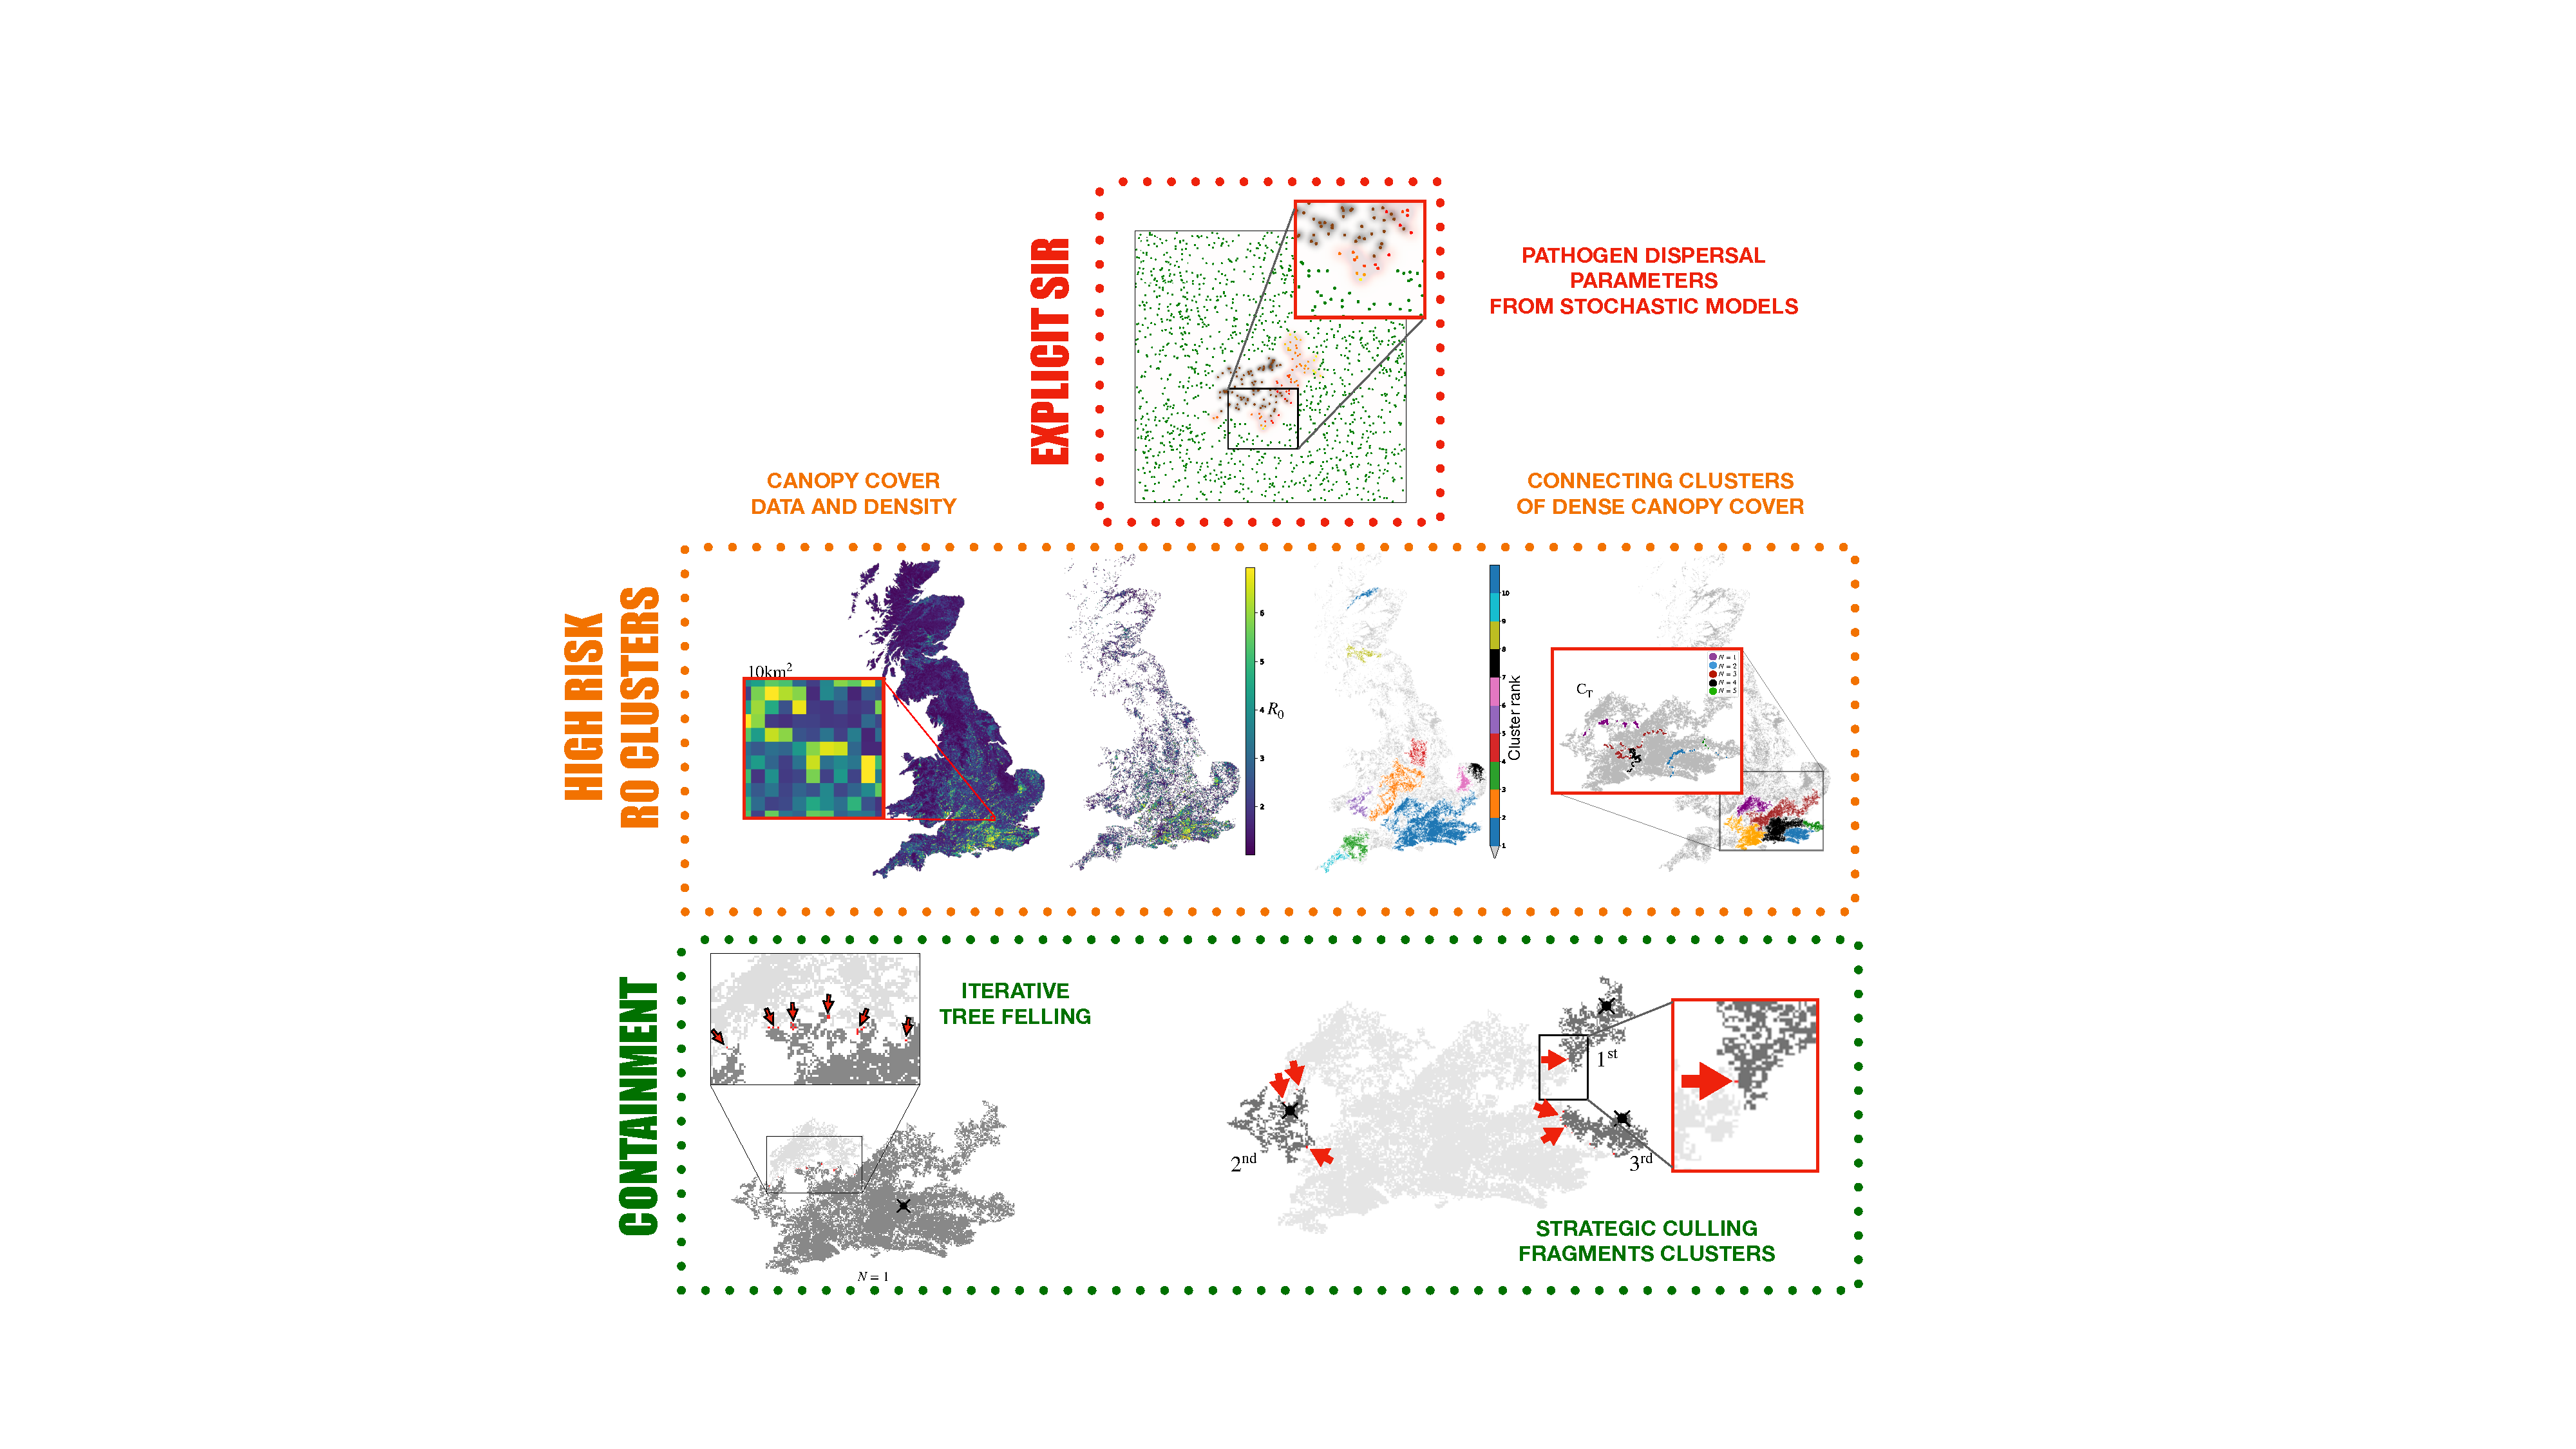
\includegraphics[scale=0.5]{appendix/Graphical_Abstract.pdf}
    \caption{Caption}
    \label{fig:my_label}
\end{figure}






% -----------------------------------------------------------------------------
% Reference list
\bibliographystyle{apalike}. 
% \bibliographystyle{acm}
\bibliography{references}
\end{document}
